%Version 3.1 December 2024
% See section 11 of the User Manual for version history
%
%%%%%%%%%%%%%%%%%%%%%%%%%%%%%%%%%%%%%%%%%%%%%%%%%%%%%%%%%%%%%%%%%%%%%%
%%                                                                 %%
%% Please do not use \input{...} to include other tex files.       %%
%% Submit your LaTeX manuscript as one .tex document.              %%
%%                                                                 %%
%% All additional figures and files should be attached             %%
%% separately and not embedded in the \TeX\ document itself.       %%
%%                                                                 %%
%%%%%%%%%%%%%%%%%%%%%%%%%%%%%%%%%%%%%%%%%%%%%%%%%%%%%%%%%%%%%%%%%%%%%

%%\documentclass[referee,sn-basic]{sn-jnl}% referee option is meant for double line spacing

%%=======================================================%%
%% to print line numbers in the margin use lineno option %%
%%=======================================================%%

%%\documentclass[lineno,pdflatex,sn-basic]{sn-jnl}% Basic Springer Nature Reference Style/Chemistry Reference Style

%%=========================================================================================%%
%% the documentclass is set to pdflatex as default. You can delete it if not appropriate.  %%
%%=========================================================================================%%

%%\documentclass[sn-basic]{sn-jnl}% Basic Springer Nature Reference Style/Chemistry Reference Style

%%Note: the following reference styles support Namedate and Numbered referencing. By default the style follows the most common style. To switch between the options you can add or remove �Numbered� in the optional parenthesis. 
%%The option is available for: sn-basic.bst, sn-chicago.bst%  
 
%%\documentclass[pdflatex,sn-nature]{sn-jnl}% Style for submissions to Nature Portfolio journals
%%\documentclass[pdflatex,sn-basic]{sn-jnl}% Basic Springer Nature Reference Style/Chemistry Reference Style
\documentclass[pdflatex,sn-mathphys-num]{sn-jnl}% Math and Physical Sciences Numbered Reference Style
%%\documentclass[pdflatex,sn-mathphys-ay]{sn-jnl}% Math and Physical Sciences Author Year Reference Style



%%\documentclass[pdflatex,sn-aps]{sn-jnl}% American Physical Society (APS) Reference Style
%%\documentclass[pdflatex,sn-vancouver-num]{sn-jnl}% Vancouver Numbered Reference Style
%%\documentclass[pdflatex,sn-vancouver-ay]{sn-jnl}% Vancouver Author Year Reference Style
%%\documentclass[pdflatex,sn-apa]{sn-jnl}% APA Reference Style
%%\documentclass[pdflatex,sn-chicago]{sn-jnl}% Chicago-based Humanities Reference Style

%%%% Standard Packages
%%<additional latex packages if required can be included here>
% 设置中文


\RequirePackage{etex}

\usepackage[UTF8]{ctex}
% \usepackage{xeCJK}
% \setCJKmainfont{Noto Serif CJK SC}
% \usepackage{unicode-math}   % 替代 amssymb + bm + fontspec

\usepackage{subfigure}
\usepackage{tabularx}
\usepackage{graphicx}
\usepackage{float}
\usepackage{epstopdf}
\usepackage{microtype}
\usepackage{enumitem}
\usepackage{multirow}
\usepackage{bbding}
\usepackage{amsmath}
% \usepackage{color}
\usepackage{bm}
\usepackage{cleveref}  
\crefname{assumption}{Assumption}{Assumptions}
\Crefname{assumption}{Assumption}{Assumptions}
% \usepackage[authoryear,sort&compress,longnamesfirst]{natbib}
\usepackage{xcolor}
\usepackage{hyperref}
\usepackage{amssymb} 
\usepackage{tikz} % Add TikZ package for diagrams
\usepackage{amsthm} 
\usepackage{booktabs}
%%%%
% 可选:让 epstopdf 自动在 \includegraphics 时启用
\epstopdfsetup{outdir=./}
%%%%%=============================================================================%%%%
%%%%  Remarks: This template is provided to aid authors with the preparation
%%%%  of original research articles intended for submission to journals published 
%%%%  by Springer Nature. The guidance has been prepared in partnership with 
%%%%  production teams to conform to Springer Nature technical requirements. 
%%%%  Editorial and presentation requirements differ among journal portfolios and 
%%%%  research disciplines. You may find sections in this template are irrelevant 
%%%%  to your work and are empowered to omit any such section if allowed by the 
%%%%  journal you intend to submit to. The submission guidelines and policies 
%%%%  of the journal take precedence. A detailed User Manual is available in the 
%%%%  template package for technical guidance.
%%%%%=============================================================================%%%%

%% as per the requirement new theorem styles can be included as shown below
\theoremstyle{thmstyleone}%
\newtheorem{theorem}{Theorem}%  meant for continuous numbers
%%\newtheorem{theorem}{Theorem}[section]% meant for sectionwise numbers
%% optional argument [theorem] produces theorem numbering sequence instead of independent numbers for Proposition
\newtheorem{proposition}[theorem]{Proposition}% 
%%\newtheorem{proposition}{Proposition}% to get separate numbers for theorem and proposition etc.
\newtheorem{lemma}{Lemma}
\newtheorem{assumption}{Assumption}
\theoremstyle{thmstyletwo}%
\newtheorem{example}{Example}%
\newtheorem{remark}{Remark}%
% \newenvironment{properties}
\newtheorem{properties}{Properties}%
\theoremstyle{thmstylethree}%
\newtheorem{definition}{Definition}%

\raggedbottom
%%\unnumbered% uncomment this for unnumbered level heads

\begin{document}

\title[Article Title]{Predefined Time Prescribed Performance Backstepping Control for Robotic Manipulators with Input Saturation}

%%=============================================================%%
%% GivenName	-> \fnm{Joergen W.}
%% Particle	-> \spfx{van der} -> surname prefix
%% FamilyName	-> \sur{Ploeg}
%% Suffix	-> \sfx{IV}
%% \author*[1,2]{\fnm{Joergen W.} \spfx{van der} \sur{Ploeg} 
%%  \sfx{IV}}\email{iauthor@gmail.com}
%%=============================================================%%

\author[1,2]{\fnm{} \sur{Shuli Liu}}\email{shunnee@163.com}
% \credit{Writing - Original Draft, Methodology, Software, Visualization, Data curation}


\author*[3]{\fnm{} \sur{Yi Liu}}\email{liuyi\_hust@163.com}
\author*[3]{\fnm{} \sur{Jingang Liu}}\email{wellbuild@126.com}
% \credit{Resources, Investigation, Formal analysis, Conceptualization, Writing - Review \& Editing}
% \equalcont{These authors contributed equally to this work.}

% \credit{Project administration, Validation, Funding acquisition, Writing - Review \& Editing}
% \equalcont{These authors contributed equally to this work.}
\author*[1,2]{\fnm{} \sur{Yin Yang}}\email{yangyinxtu@xtu.edu.cn}
% \credit{Supervision, Funding acquisition, Writing - Review \& Editing}
% \equalcont{These authors contributed equally to this work.}

\affil[1]{\orgname{School of Mathematics and Computational Science, Xiangtan University}, \orgaddress{\street{Street}, \city{City}, \postcode{411105}, \country{China}}}

\affil[2]{\orgname{National Center for Applied Mathematics in Hunan}, \orgaddress{\street{Street}, \city{City}, \postcode{411105}, \country{China}}}

\affil[3]{\orgname{School of Mechanical Engineering and Mechanics, Xiangtan University}, \orgaddress{\street{Street}, \city{City}, \postcode{411105}, \country{China}}}



% Here goes the abstract
\abstract{

% 面向具有未知动力学、有界扰动以及输入饱和的机械臂轨迹跟踪,本文提出一种融合预定义时间收敛与全局预设性能约束的自适应反步控制方法。按通道独立设计的预定义时间误差变换将多项式性能函数与误差缩放结合,消除传统PPC中的初值奇异与非光滑问题,使系统在未知初始状态下仍能在给定时间内平滑地满足全过程约束;

% 针对传统预设性能控制中存在的初值奇异性和误差变换非光滑问题,针对每个通道独立设计了结合多项式性能函数与误差缩放函数的预定义时间误差变换结构,确保系统状态在预定义时间内严格且平滑地满足全局预设性能约束。构造统一饱和补偿器,同步抵消命令滤波与执行器饱和残差,抑制反步结构的“复杂性爆炸”,降低在线计算;引入一阶滑模扰动观测器与RBFNN对有界扰动与未建模动态进行在线辨识与补偿,增强鲁棒性与跟踪精度;结合预定义时间稳定性与自适应动态障碍Lyapunov工具,严格证明闭环按时收敛与全局有界。数值和实验结果验证了所提出方法与现有方法相比,本文方法在响应速度、稳态精度等性能方面表现出明显优势。

For robotic manipulators trajectory tracking with unknown dynamics, bounded disturbances, and input saturation, this work proposes an adaptive backstepping control method that combines predefined time convergence with global predefined performance constraints. A channel-wise predefined-time error transformation merges a polynomial performance function with error scaling. It removes initial-state singularities and nonsmooth mappings in conventional PPC and enforces strict, smooth, global bounds within a user-set time, even from unknown initial states. We also design a unified saturation compensator that cancels residuals from command filtering and actuator saturation, curbs the backstepping complexity explosion, and reduces online computation. A first-order sliding-mode disturbance observer and an RBFNN estimator run online to handle bounded disturbances and unmodeled dynamics. With predefined-time stability theory and an adaptive dynamic barrier Lyapunov function, we prove closed-loop boundedness and on-time convergence. Simulations and experiments show faster response, better steady-state accuracy, and stronger robustness than existing methods.


}
\keywords{Prescribed performance control, predefined-time stability, adaptive dynamic barrier Lyapunov function, backstepping control, input saturation, robotic manipulators' trajectory tracking.
}
\maketitle

% Main text
\section{Introduction}\label{intro}



% 机器人机械臂凭借其高精度和柔性特性,广泛应用于工业装配、航天探测、医疗手术等高要求场景 \cite{SciaviccoSiciliano_2012_ModellingControl,BagheriEtAl_2019_Feedbacklinearization}。机械臂通常需要在有限时间内完成高精度轨迹跟踪,其动力学系统常伴随强非线性、多输入多输出耦合及显著不确定性,且常伴随有界扰动与执行器饱和 \cite{Spong_2022_historicalperspective, SciaviccoSiciliano_2012_ModellingControl}。若控制不当,极易导致误差放大、响应迟缓,甚至系统失稳。在不确定性条件下实现整个轨迹跟踪过程中误差的有效约束,并使其在严格规定的时间内收敛,是当前控制研究的重要问题。围绕上述目标,研究者们已提出诸多控制策略,包括PID反馈控制 \cite{ShojaeiEtAl_2021_ObserverBasedNeural,BagheriEtAl_2019_Feedbacklinearization}、自适应控制 \cite{ZhouEtAl_2022_Adaptivefinitetime,XuHe_2023_Robustadaptive,WangYang_2017_Dynamiclearning}、滑模控制 \cite{ZhangEtAl_2024_noveldisturbance,YangSu_2022_Proximatefixedtime, ZhaiLi_2022_Fastexponentialsliding}、模型预测控制 \cite{IncremonaEtAl_2017_MPCrobot}、强化学习控制 \cite{CaoEtAl_2023_ReinforcementLearningBased,WuEtAl_2024_TransferReinforcement} 等。然而,传统渐近型方法难以保证收敛时限,且对误差边界与饱和的显式约束不足。

% 为缓解上述不足,利用神经网络(NN)\cite{LiuEtAl_2018_Adaptiveneural} 、模糊逻辑系统(FLS)\cite{LiuEtAl_2025_Fuzzyadaptive}和自适应法则 \cite{WangEtAl_2022_Adaptiveactuator} 对未知非线性进行实时逼近。基于扰动观测器的补偿控制、高阶滑模控制以及边界层等技术被广泛引入。众所周知,传统渐近稳定控制方法在理论上的收敛时间可能无限长,难以满足实际应用对快速动态响应的严格需求 \cite{BacciottiRosier_2005_Liapunovfunctions}。因此,有限时间控制(Finite-Time Control, FTC)理论逐渐引入,实现非线性系统的快速稳定控制 \cite{SongLi_2024_Generallyapunov,LiuEtAl_2022_overviewfinite,SongEtAl_2023_Finitetimeadaptive}。然而,这类控制方案的收敛特性依赖初始条件,初始误差较大时收敛时间显著延长,难以满足严格的时域控制要求。针对收敛时间不可预测的问题,学者们提出了固定时间控制(FxTC)确保系统收敛时间的上界独立于初始状态,解决初始条件带来的收敛时间不确定性问题 \cite{Polyakov_2012_Nonlinearfeedback}。但其收敛时间上界完全由控制参数决定,无法由用户直接指定特定的收敛时刻 \cite{YangSu_2022_Proximatefixedtime,ZhangEtAl_2023_Globalcomposite}。为克服这一局限,related work 提出了预定义时间稳定性理论,在控制器中显式引入收敛时间参数,使得收敛时间上界能够由用户任意设定, 且与初始条件无关 \cite{GuoEtAl_2023_Predefinedtimestability,FanEtAl_2024_predefinedtime,WangEtAl_2022_Adaptivefuzzy}。PTC在对时域性能要求严格的电力系统与机器人控制等领域中迅速获得广泛关注 \cite{SunEtAl_2022_NeuralNetworkBased,WangEtAl_2022_Adaptivefuzzy,LiEtAl_2024_Adaptivepractical,ShenEtAl_2024_Predefinedtimeeventtriggered}。

% % \cite{BechlioulisRovithakis_2008_Prescribedperformance,BechlioulisRovithakis_2008_Robustadaptive,BechlioulisRovithakis_2010_Prescribedperformance,BechlioulisRovithakis_2012_Robustadaptive,BechlioulisRovithakis_2011_Robustpartialstate,Bu_2023_Prescribedperformance}
% 另一方面,为严格限定轨迹跟踪过程中的瞬态性能与稳态精度,预设性能控制(PPC)通过误差映射确保误差始终处于设计包络内,可显著抑制超调并提升收敛质量 \cite{BechlioulisRovithakis_2008_Prescribedperformance,Bu_2023_Prescribedperformance}。实质上,PPC提供了一种系统化的预规划机制,确保运行过程中跟踪误差被严格约束在设计指标范围内 \cite{ZhangEtAl_2024_Prescribedperformance,ZhangEtAl_2024_Lowcomplexityprescribed,ZhangChai_2023_Globalprescribed}。与势垒李雅普诺夫函数(BLFs)结合可进一步提升安全性与鲁棒性 \cite{WangEtAl_2024_Prescribedperformance,XieEtAl_2024_Lowcomplexitytracking}。该方法及其变种已被成功应用于机器人及其他非线性系统\cite{DimanidisEtAl_2020_Outputfeedback,WangEtAl_2024_Adaptivefaulttoleranta,LiuEtAl_2023_Reducedorderobserverbased,DimanidisEtAl_2020_Outputfeedback}。然而,误差变换在边界附近可能奇异或非光滑,且常隐含要求初始误差位于包络内,难以处理高速冲击的工程问题。且传统PPC与BLF方法往往仅保证误差渐近收敛,缺乏时间收敛控制能力。近期研究开始探索将预设性能与有限时间控制相结合,以兼顾收敛质量与时间指标 \cite{LiuEtAl_2018_Adaptiveneural,SuiEtAl_2022_Finitetimeadaptive,SunEtAl_2022_Fuzzyadaptive,SongZhou_2018_NeuroadaptiveControl,GaoEtAl_2023_Finitetimefaulttolerant}。例如,Liu 等提出了基于PPC的自适应神经网络有限时间控制方案 \cite{LiuEtAl_2018_Adaptiveneural};Zhang 等设计了具有全局有限时间稳定性的自适应PPC策略,应用于机械臂跟踪控制 \cite{ZhangEtAl_2024_noveldisturbance}。与此同时,有相关工作将固定时间控制与预设性能约束结合 \cite{LiEtAl_2023_Distributedfixedtime,ZhuEtAl_2023_Fixedtimefuzzy,SunEtAl_2024_Fixedtimeprescribed,YangEtAl_2023_Proximatefixedtime,ZhangEtAl_2023_Globalcomposite}。例如,Zhou 等提出了一种用于参数时变非线性系统的固定时间PPC控制方案 \cite{SunEtAl_2024_Fixedtimeprescribed},Yang 等设计了具备PPC功能的近似固定时间容错跟踪控制策略 \cite{YangEtAl_2023_Proximatefixedtime,YangSu_2022_Proximatefixedtime},Zhang 等开发了适用于机器人系统的全局复合学习固定时间控制框架,并引入非对称误差约束 \cite{ZhangEtAl_2023_Globalcomposite}。然而,这些方法对初始条件仍敏感,难以确保在大初值误差条件下快速满足预期性能,且无法显式设置收敛时限。

% 尽管已有少量work开始探索PTC与PPC相结合,但整体上仍缺乏统一完备的理论框架。例如,Wang 等围绕非合作航天器接管任务给出了非奇异预定义时间终端滑模与新型性能函数,实现姿态误差的定量约束 \cite{WangEtAl_2023_Predefinedtimeguaranteed};Yao 等针对带输入时延的随机非线性系统提出了基于PTC与性能函数的切换误差变换,突破了传统 PPC 需将初值置于包络内的限制 \cite{YaoEtAl_2024_Prescribedtimeprescribed};Liu 等将模糊自适应与预定义时间性能函数结合,获得在不确定扰动下的全局 PPC 控制 \cite{LiuEtAl_2025_Fuzzyadaptive}。但这些研究普遍未系统纳入执行器饱和与关节速度显式约束。实际中,若饱和非线性处理不当,轻则性能显著劣化,重则诱发超调甚至失稳。更关键的是,性能约束与状态/输入饱和能力约束相互耦合,收紧边界会推高控制需求并触发饱和,而饱和又可能逼迫误差逼近或跨越边界。近年来有相关工作提出柔性PPC,在接近饱和时临时放宽边界、脱离后再收紧,以在线权衡可实现性与性能 \cite{Bu_2023_Hypersonic,Yao_2024_Flexible}. 另一方面,安全动态包络增强的 PPC 通过饱和检测与安全域调度抑制边界与饱和的相互激化 \cite{Wang_2025_Enhanced}。也有相关工作提出基于性能函数再调整与抗饱和补偿的等效处理,将饱和等价为可管控输入并保持 PPC 的约束优势 \cite{Wang_2023_Adaptive,ElikerJouffroy_2025_robustquadrotor}。尽管如此,现有方法仍少有在同一框架内同时实现用户可设的预定义时间收敛与全过程性能约束,并以显式且低复杂度的方式处理饱和问题。

% 基于上述挑战,本文提出一种融合预定义时间稳定性与预设性能约束的自适应反步控制方法.主要贡献如下:(i)按通道独立的预定义时间误差变换,将多项式性能函数与误差缩放耦合,系统性消除 PPC 中的初值奇异与非光滑问题,实现对未知初态的平滑合法化与严格控时的全过程约束;(ii)设计统一的预定义时间饱和补偿器,同时抵消命令滤波与执行器饱和残差,抑制反步结构复杂性爆炸,降低在线计算与增益需求;(iii)采用一阶滑模扰动观测器补偿有界扰动与 RBFNN 在线辨识补偿未建模动态;(iv)基于预定义时间稳定性与自适应动态障碍 Lyapunov 工具,严格证明闭环系统在预设时间内的全局稳定与误差收敛。多自由度机械臂平台的仿真与实验验证显示,所提方法在大初始偏差在预定义时间内达成性能约束以及扭矩需求与抖振抑制方面,均优于对比控制策略,体现良好的理论可推广性与工程可实施性。



% \section{Problem statement and preliminaries}
\section{Problem and preliminary}


\subsection{System description}
\par This work considers an uncertain nonlinear n-DOF robot manipulators system. Its dynamics are described as \cite{SciaviccoSiciliano_2012_ModellingControl,BagheriEtAl_2019_Feedbacklinearization}:
\begin{equation}
	M(q)\ddot{q} + C(q, \dot{q})\dot{q} + G(q)+ \Delta(q, \dot{q}, t)= \tau + d(t),
	\label{eq:1}
\end{equation}
where $ q, \dot{q}, \ddot{q} \in \mathbb{R}^n $ are the joint state vectors, $M(q) \in \mathbb{R}^{n\times n}$ is the inertia matrix, $C(q, \dot{q}) \in \mathbb{R}^{n\times n} $ represents the centrifugal effects, $G(q) \in \mathbb{R}^n $ represents the gravitational force, $\tau \in \mathbb{R}^n$ is the control joint input, $\Delta(q, \dot{q}, t) \in \mathbb{R}^n$ is the uncertainty and unmodeled dynamics, $d(t) \in \mathbb{R}^n$ is an external disturbance, $n$ is the number of DOF of the manipulators system.

For controller design, define the state $x = [x_1,x_2] = [q,\dot{q}] \in \mathbb{R}^{2n}$. The system \cref{eq:1} can be written in the standard state space form:
\begin{equation}
	\left\{
	\begin{aligned}
		\dot{x}_1 & = x_2,     \\
		\dot{x}_2 & =f +g \bar{u} +h,
	\end{aligned}
	\right.
	\label{eq:2}
\end{equation}
where $f=-M^{-1}(q) (C(q,\dot{q})x_2 + G(q)) $, $g=M^{-1}(q)$, $h=-M^{-1}(q)(\Delta(q,\dot{q},t) - d(t))$, and $x_1=[x_{1,1},x_{2,1},...,x_{n,1}]^{\top}$, $x_2=[x_{1,2},x_{2,2},...,x_{n,2}]^{\top}$, $\bar{u}$ denotes control input saturation. Define the saturation error as
\begin{equation}\label{eq:3}
\Delta u_{i} =  u_{i}-\bar{u}_{i}=\begin{cases} 
	u_{i}-u_{\max}, & u_i \geq u_{\max}, \\
0,       & u_{\min} < u_i < u_{\max},  \quad i=1,2,...,n,\\
u_{i}-u_{\min}, & u_i \leq u_{\min},
\end{cases}
\end{equation}
where $u_{\max},u_{\min}$ are the upper and lower saturation bounds of control input, respectively.

\par The controller design and stability analysis are conducted under the following physically justified assumptions.
\begin{assumption}\cite{Spong_2022_historicalperspective}   \label{assumption:1}
	$M(q)$ is symmetric positive definite for all $q$. There exist constants $m_1,m_2>0$ such that
	$m_1 I \le M(q) \le m_2 I,\ \forall q\in\mathbb{R}^n$.
	Moreover, the standard structural property holds: $\dot M(q)-2C(q,\dot q)$ is skew-symmetric.
	\end{assumption}
	
	\begin{assumption}  \label{assumption:2}
	The unmodeled dynamics are bounded: there exists $\bar{\Delta}>0$ such that
	$\|\Delta(q,\dot q,t)\|\le \bar{\Delta}$, $\forall t\ge 0$.
	The disturbance and its derivative are bounded: there exist $\bar d,\bar{\dot d}>0$ such that
	$\|d(t)\|\le \bar d$ and $\|\dot d(t)\|\le \bar{\dot d}$, $\forall t\ge 0$.
	The desired trajectory $q_d(t)$ is twice continuously differentiable, and there exist
	$\bar q_d,\bar{\dot q}_d,\bar{\ddot q}_d>0$ such that
	$\|q_d(t)\|\le \bar q_d$, $\|\dot q_d(t)\|\le \bar{\dot q}_d$,
	$\|\ddot q_d(t)\|\le \bar{\ddot q}_d$, $\forall t\ge 0$.
	\end{assumption}
% \begin{assumption} \cite{Spong_2022_historicalperspective}
%  $M(q)$ of the system is symmetric positive definite for all $q$, and there exist positive constants $m_1, m_2 > 0$ that satisfy: 
% \( m_1 I \leq M(q) \leq m_2 I, \forall q \in \mathbb{R}^n \), and at the same time the system satisfies structural property: \( \dot{M}(q) - 2C(q, \dot {q})\) is an antisymmetric matrix.
% \end{assumption}
% \begin{assumption}
% 	The unmodeled dynamic $\Delta(q, \dot{q}, t)$ is bounded, there exists \( \|\Delta(q, \dot{q}, t)\| \leq \bar{\Delta}, \forall t \geq 0\). The external disturbance $d(t)$ and its derivative are both bounded, and there exist \( \|d(t)\| \leq \bar{d},\|\dot{d}(t)\| \leq \bar{\dot{d}}, \forall t \geq 0\). $\bar{\Delta}, \bar{d}, \bar{\dot{d}}$ are the positive constants.
% \end{assumption}
% \begin{assumption}
% 	The desired trajectory function $q_d(t)$ and its first and second order derivatives are continuously differentiable functions and there exist positive constants $\bar{q}_d, \bar{\dot{q}}_d, \bar{\ddot{q}}_d$ that satisfy:
% 	\(\|q_d(t)\| \leq \bar{q}_d, \|\dot{q}_d(t)\| \leq \bar{\dot{q}}_d, \|\ddot{q}_d(t)\| \leq \bar{\ddot{q}}_d, \forall t \geq 0\).
% \end{assumption}







% \subsection{Radial basis function neural network}




% \par RBFNN is a universal approximator on compact sets and is widely employed to estimate unknown nonlinear functions \cite{SunEtAl_2022_NeuralNetworkBased, SongZhou_2018_NeuroadaptiveControl}. The input to the RBFNN is defined as $\chi$, the output of the network denoted as $h_i$, is expressed as
% \begin{equation}
% 	h_i={w_i^*}^{T} { Q_i} (\chi)+\varepsilon_i, 
% 	\label{eq:4}
% \end{equation}
% where ${{w_i^*}}\in \mathbb{R}^N, w_i^*=[{{w}_{i,1}},{{w}_{i,2}},\cdots,{{w}_{i,N}}]^{T}$ is the idea weight vector, $Q_i(\chi)\!\in\mathbb{R}^N$ is the vector of basis functions, and $\varepsilon_i$ is the approximation error satisfying $|\varepsilon_i|\le \bar\varepsilon$ for all $\chi$ in a compact set $\Omega_\chi\subset\mathbb{R}^m$, with a known constant $\bar\varepsilon>0$. ${ Q_i}(\chi)=[{{ Q}_{i,1}( \chi )}, {{ Q_{i,2}}( \chi )}, \cdots,{{ Q_{i,N}}( \chi )}]^{T}$ is the activation function of the hidden layer neurons. The base function \( { Q}_{i,\ell }( \chi ) \) is
% \begin{equation}
% 	{ Q}_{i,\ell}( \chi ) =\operatorname{exp} \biggl(-\frac{\left\| \chi-o_{\ell} \right\|^2} { D_{\ell}^2} \biggr), \quad \ell=1, 2,..., N,
% 	\label{eq:5}
% \end{equation}
% where $o_\ell\in\mathbb{R}^m$ and $D_\ell>0$ denote the center and width of the Gaussian basis, respectively; $N$ is the number of neurons.

% % \par Define $\tilde{w}_i = w_i^*-\hat{w}_i$, where $\tilde{w}_i$ is the weight estimation. To ensure the validity of the weight adaptation process, the ideal weight $w_i^*$ should minimize the approximate error \( \varepsilon_i \), that is
% \par Let $\hat w_i$ be the adaptive estimate of $w_i^*$ and define the weight estimation error $\tilde w_i= w_i^*-\hat w_i$. The ideal weight $w_i^*$ is understood as the best fixed parameter within the chosen basis that minimizes the worst-case approximation error over $\Omega_\chi$:
% \begin{equation}
% 	w_i^* = \arg \min_{w_i \in \mathbb{R}^N} \left\{ \sup_{\chi \in \Omega_\chi} | f_i(\chi) - w_i^{\top}  Q_i(\chi) | \right\}.
% 	\label{eq:6}
% \end{equation}

% \begin{assumption}\label{assumption:3}
% 	The optimal weight vector $w_i^*$ is bounded, and there exists \(\| w_i^* \| \leq \bar{w}\), $\bar{w} > 0$.
% \end{assumption}


 


\subsection{Fuzzy logic system }
\par Fuzzy logic systems (FLS) are universal approximators on compact sets and are widely employed to estimate unknown nonlinear mappings. Let the regressor be $\chi\in\mathbb{R}^m$. For the $i$-th channel, an FLS with $N$ Takagi--Sugeno rules (singleton fuzzifier, product inference, and center-average defuzzifier) is constructed as:
\begin{center}
\emph{Rule $\ell$: If $\chi_1$ is $A_{1\ell}$ and $\cdots$ and $\chi_m$ is $A_{m\ell}$, then $y_i$ is $\theta_{i,\ell}$}, \quad $\ell=1,\dots,N$,
\end{center}
where $\theta_{i,\ell}\in\mathbb{R}$ are consequent parameters to be learned. Denote the normalized basis vector by
\(
\psi_i(\chi)=\big[\psi_{i,1}(\chi),\dots,\psi_{i,N}(\chi)\big]^\top\in\mathbb{R}^N.
\)
Then the FLS output used to approximate the unknown $f_i(\chi)$ is modeled as
\begin{equation}
    h_i \;=\; {\theta_i^*}^{\!\top}\,\psi_i(\chi)\;+\;\varepsilon_i,
    \label{eq:4}
\end{equation}
where $\theta_i^*=[\theta_{i,1}^*,\dots,\theta_{i,N}^*]^\top\in\mathbb{R}^N$ is the ideal parameter vector within the chosen rule base, and $\varepsilon_i$ is the bounded approximation error satisfying $|\varepsilon_i|\le\bar\varepsilon$ for all $\chi$ in a compact set $\Omega_\chi\subset\mathbb{R}^m$, with a known constant $\bar\varepsilon>0$.

\par The normalized basis functions $\psi_{i,\ell}(\chi)$ are computed from the firing strengths $\varpi_\ell(\chi)$:
\begin{equation}
    \psi_{i,\ell}(\chi)\;=\;\frac{\varpi_\ell(\chi)}{\sum_{k=1}^N \varpi_k(\chi)},
    \quad
    \varpi_\ell(\chi)\;=\;\prod_{j=1}^m \mu_{j,\ell}(\chi_j),
    \quad \ell=1,\dots,N,
    \label{eq:5}
\end{equation}
where $\mu_{j,\ell}(\cdot)$ are the membership functions of the antecedent fuzzy sets $A_{j,\ell}$. In this paper we choose Gaussian membership functions
\[
\mu_{j,\ell}(\chi_j)\;=\;\exp\!\Big(-\frac{(\chi_j-\mathcal{C}_{j,\ell})^2}{\mathcal{D}_{j,\ell}^2}\Big),\quad
\mathcal{C}_{j,\ell}\in\mathbb{R},\ \mathcal{D}_{j,\ell}>0,
\]
with $\mathcal{C}_{j,\ell}$ and $\mathcal{D}_{j,\ell}$ denoting the centers and widths, respectively.

\par Let $\hat\theta_i$ be the adaptive estimate of $\theta_i^*$ and define the parameter estimation error $\tilde\theta_i=\theta_i^*-\hat\theta_i$, $\hat\theta_i(0)= 0$. The ideal parameter vector $\theta_i^*$ is understood as the best fixed parameter within the chosen rule base that minimizes the worst-case approximation error over $\Omega_\chi$:
\begin{equation}
    \theta_i^* \;=\; \arg\min_{\theta_i\in\mathbb{R}^N}
    \left\{\,\sup_{\chi\in\Omega_\chi}\, \big|\, f_i(\chi)-\theta_i^\top \psi_i(\chi)\,\big| \right\}.
    \label{eq:6}
\end{equation}

\begin{assumption}\label{assumption:3}
The ideal parameter vector $\theta_i^*$ is bounded, i.e., there exists $\bar\theta>0$ such that $\|\theta_i^*\|\le \bar\theta$.
\end{assumption}


仿真参数设置:
The parameters of FLS are set as $N=25$, $\mathcal C_{j,\ell}\in\{-1,\,-0.5,\,0,\,0.5,\,1\}$, $\mathcal D_{j,\ell}=0.4$, $\bar\theta=50$, $\varrho_i=15$, $\kappa_i=0.05$。




% \subsection{模糊逻辑系统(FLS)}
% \par 模糊逻辑系统(FLS)在紧集上具有通用逼近能力,常用于对未知非线性映射进行估计。设回归向量为 $\chi\in\mathbb{R}^m$。针对第 $i$ 个通道,构造包含 $N$ 条 Takagi--Sugeno 规则(单点隶属化、乘积推理、中心平均解模糊)的 FLS:
% \begin{center}
% \emph{规则 $\ell$: 若 $\chi_1$ 属于 $A_{1\ell}$ 且 $\cdots$ 且 $\chi_m$ 属于 $A_{m\ell}$,则 $y_i$ 为 $\theta_{i,\ell}$}, \quad $\ell=1,\dots,N$,
% \end{center}
% 其中 $\theta_{i,\ell}\in\mathbb{R}$ 为后件参数。记归一化基向量(归一化的触发强度)为
% \[
% \Psi_i(\chi)=\big[\psi_{i,1}(\chi),\dots,\psi_{i,N}(\chi)\big]^\top\in\mathbb{R}^N.
% \]
% 则用于逼近未知函数 $f_i(\chi)$ 的 FLS 输出记为
% \begin{equation}
%     h_i \;=\; {\theta_i^*}^{\!\top}\,\psi_i(\chi)\;+\;\varepsilon_i,
%     \label{eq:4}
% \end{equation}
% 其中 $\theta_i^*=[\theta_{i,1}^*,\dots,\theta_{i,N}^*]^\top\in\mathbb{R}^N$ 为在所选规则库下的(未知)理想参数向量,$\varepsilon_i$ 为逼近误差,满足对所有 $\chi\in\Omega_\chi\subset\mathbb{R}^m$(紧集)都有 $|\varepsilon_i|\le\bar\varepsilon$,其中 $\bar\varepsilon>0$ 为已知常数。

% \par 归一化基函数 $\psi_{i,\ell}(\chi)$ 由未归一化触发强度 $\varpi_\ell(\chi)$ 得到:
% \begin{equation}
%     \psi_{i,\ell}(\chi)\;=\;\frac{\varpi_\ell(\chi)}{\sum_{k=1}^N \varpi_k(\chi)},
%     \quad
%     \varpi_\ell(\chi)\;=\;\prod_{j=1}^m \mu_{j,\ell}(\chi_j),
%     \quad \ell=1,\dots,N,
%     \label{eq:5}
% \end{equation}
% 其中 $\mu_{j,\ell}(\cdot)$ 为前件模糊集 $A_{j,\ell}$ 的隶属函数。本文选用高斯型隶属函数
% \[
% \mu_{j,\ell}(\chi_j)\;=\;\exp\!\Big(-\frac{(\chi_j-\mathcal{C}_{j,\ell})^2}{\mathcal{D}_{j,\ell}^2}\Big),\quad
% \mathcal{C}_{j,\ell}\in\mathbb{R},\ \mathcal{D}_{j,\ell}>0,
% \]
% 其中 $\mathcal{C}_{j,\ell}$ 与 $\mathcal{D}_{j,\ell}$ 分别表示中心与宽度。

% \par 记 $\hat\theta_i$ 为 $\theta_i^*$ 的自适应估计,并定义参数估计误差 $\tilde\theta_i=\theta_i^*-\hat\theta_i$,。理想参数向量 $\theta_i^*$ 定义为在给定规则/基函数下,使得在 $\Omega_\chi$ 上最坏情形逼近误差最小的固定参数:
% \begin{equation}
%     \theta_i^* \;=\; \arg\min_{\theta_i\in\mathbb{R}^N}
%     \left\{\,\sup_{\chi\in\Omega_\chi}\, \big|\, f_i(\chi)-\theta_i^\top \psi_i(\chi)\,\big| \right\}.
%     \label{eq:6}
% \end{equation}

% \begin{assumption}\label{assumption:3}
% 理想参数向量 $\theta_i^*$ 有界,即存在常数 $\bar\theta>0$ 使得 $\|\theta_i^*\|\le \bar\theta$。
% \end{assumption}




\subsection{Preliminary}


\begin{lemma} \label{lemma:1}\cite{WangEtAl_2022_Adaptivefuzzy} (Predefined time stable theory). Consider the system $
	\dot{x}(t) = f(x(t)), x(0) = x_0
$, where $x \in \mathbb{R}^n$ is the system's state, and $x(0) = x_0$ is the initial state. $f(\cdot)$ is continuous and satisfies $f(0) = 0$. et $V:\mathbb{R}^n\to\mathbb{R}_+$ be continuously differentiable, positive definite, and radially unbounded, with $V(0)=0$ and $V(x)>0$ for all $x\neq 0$.
For given design parameters $0<\eta<1$, $T_p>0$, and $0<\varsigma<\infty$, suppose the closed-loop system satisfies
			  
% Suppose there is a continuously differentiable, positive definite, and radially unbounded function $V(x)$, for some constants \(0<\eta<1,T_p>0, 0<\varsigma<\infty\), the closed-loop system satisfies
% Consider a continuously differentiable, positive definite, and radially unbounded Lyapunov function candidate \( V(x) : \mathbb{R}^n \rightarrow \mathbb{R}_+ \) satisfying \( V(0) = 0 \) and \( V(x) > 0 \) for all \( x \neq 0 \). For given design parameters \( 0 < \eta < 1 \), \( T_p > 0 \), and \( 0 < \varsigma < +\infty \), the closed-loop system is designed to satisfy the following stability condition: 
\begin{equation}	\label{eq:7}
	\dot V(x) \le
	-\,\frac{\pi}{\eta\,T_p}\left(V(x)^{\,1-\frac{\eta}{2}}+V(x)^{\,1+\frac{\eta}{2}}\right)
	+\varsigma,
\end{equation}
Then the origin is predefined-time stable with convergence time bounded by $T_p$. Moreover,
\begin{equation}\label{eq:8}
	\Biggl\{ \lim_{t\to T_p} x|V
	\le
	\min\!\Biggl\{\,
	\left(\tfrac{2\,\eta\,T_p\,\varsigma}{\pi}\right)^{\frac{1}{1-\frac{\eta}{2}}}\!,
	\left(\tfrac{2\,\eta\,T_p\,\varsigma}{\pi}\right)^{\frac{1}{1+\frac{\eta}{2}}}
	\Biggr\} \Biggr\},
\end{equation}
In particular, if $\varsigma=0$ then $V(T_p)=0$.
\end{lemma}



\begin{definition}[PTS--ISS]\label{def:PTS-ISS}
	考虑系统 $\dot x = f(x,u)$。若存在给定常数 $T>0$、$\eta\in(0,1)$ 以及类-$\mathcal{K}$ 函数 $\gamma(\cdot)$,使得对任意本质有界输入 $u\in L_\infty$,
	\[
	\|x(T)\|\ \le\ \gamma\big(\|u\|_\infty\big),
	\]
	并且对所有 $t\ge T$ 状态保持在该球内;若 $u\equiv 0$ 则 $x(T)=0$。则称系统在预定义时间 $T$ 满足输入到状态稳定(Predefined-Time ISS, 简记 PTS--ISS)。
	\end{definition}
	
	\begin{theorem}[PTS--ISS 的 Lyapunov 判据]\label{thm:PTS-ISS}
	设存在 $C^1$ Lyapunov 函数 $V:\mathbb{R}^n\to\mathbb{R}_+$ 与类-$\mathcal{K}_\infty$ 函数 $\alpha_1,\alpha_2$ 使得
	\[
	\alpha_1(\|x\|)\ \le\ V(x)\ \le\ \alpha_2(\|x\|),\quad V(0)=0,
	\]
	并存在给定参数 $T>0,\ \eta\in(0,1)$ 以及类-$\mathcal{K}$ 函数 $\sigma(\cdot)$,使对所有 $(x,u)$ 成立
	\begin{equation}\label{eq:PTS-ISS-core}
	\dot V(x,u)\ \le\ -\,\frac{\pi}{\eta\,T}\Big(V^{\,1-\frac{\eta}{2}}+V^{\,1+\frac{\eta}{2}}\Big)\ +\ \sigma\big(\|u\|_\infty\big).
	\end{equation}
	则对任意初值与本质有界输入 $u$,在 $t=T$ 时
	\begin{equation}\label{eq:PTS-ISS-bound}
	V(T)\ \le\ \min\!\left\{
	\Big(\tfrac{2\eta T}{\pi}\,\sigma(\|u\|_\infty)\Big)^{\!\frac{1}{\,1-\frac{\eta}{2}\,}},
	\ \ 
	\Big(\tfrac{2\eta T}{\pi}\,\sigma(\|u\|_\infty)\Big)^{\!\frac{1}{\,1+\frac{\eta}{2}\,}}
	\right\},
	\end{equation}
	并且对所有 $t\ge T$ 有 $V(t)\le V(T)$。若 $u\equiv 0$(从而 $\sigma(0)=0$),则 $V(T)=0$,即系统在预定义时间 $T$ 到达原点。
	\end{theorem}
	
	\begin{proof}
	令 $r:=\|u\|_\infty$,则 $\sigma(\|u\|_\infty)=\sigma(r)$ 为常数。由 \cref{eq:PTS-ISS-core} 得
	\[
	\dot V\ \le\ -\,\frac{\pi}{\eta\,T}\Big(V^{\,1-\frac{\eta}{2}}+V^{\,1+\frac{\eta}{2}}\Big)\ +\ \sigma(r).
	\]
	考虑比较系统
	\[
	\dot z\ =\ -\,\frac{\pi}{\eta\,T}\Big(z^{\,1-\frac{\eta}{2}}+z^{\,1+\frac{\eta}{2}}\Big)\ +\ \sigma(r),\quad z(0)=V(0).
	\]
	由比较引理得 $V(t)\le z(t)$。对该标量系统应用预定义时间引理(即原文的 Lemma~1,将常数项 $\varsigma$ 替换为 $\sigma(r)$),即可得到 \cref{eq:PTS-ISS-bound}。进一步令
\[
V^\star(r):=\min\!\left\{
\Big(\tfrac{2\eta T}{\pi}\,\sigma(r)\Big)^{\!\frac{1}{1-\frac{\eta}{2}}},
\ \ 
\Big(\tfrac{2\eta T}{\pi}\,\sigma(r)\Big)^{\!\frac{1}{1+\frac{\eta}{2}}}
\right\},
\]
则当 $V>V^\star(r)$ 时右端严格为负,故 $V$ 下降;当 $V\le V^\star(r)$ 时解不能越出该阈值。由于 $V(T)\le V^\star(r)$,于是对所有 $t\ge T$ 有
\[
V(t)\ \le\ V^\star(\|u\|_\infty).
\]
若 $u\equiv0$(从而 $\sigma(0)=0$),则 $V^\star(0)=0$ 且 $V(T)=0$。证毕。

	\end{proof}
	
	\begin{remark}[与原 Lemma 1(预定义时间稳定)的对比]
	\begin{itemize}
	  \item \textbf{扰动建模层级:} Lemma 1 要求
	  $\dot V \le -\frac{\pi}{\eta T_p}(V^{1-\eta/2}+V^{1+\eta/2})+\varsigma$,其中 $\varsigma$ 为常数;
	  本定理将该常数推广为输入范数的类-$\mathcal{K}$ 函数 $\sigma(\|u\|_\infty)$,从而可统一刻画外界扰动、建模不确定性、近似残差、饱和残差、滤波导数等所有残余影响(将其堆叠为“输入”并取 $\|\cdot\|_\infty$)。
	  \item \textbf{结论形式:} 两者在 $t=T$ 都给出闭式“进入并保持”的半径;当 $u\equiv0$(或 $\sigma(0)=0$)时,本定理退化为 Lemma 1 的“预定义时间到原点”结论;当 $u\not\equiv0$ 而有界时,本定理给出预定义时间一致实用稳定(半径由 $\sigma(\|u\|_\infty)$ 决定),而 Lemma 1 只能处理常数半径。
	  \item \textbf{可设定时间:} 两者右端均含“双幂核” $V^{1\mp\eta/2}$,系数 $\pi/(\eta T)$ 直接将到达/进入时间预设为 $T$;若工程上得到
	  $\dot V\le -c\big(V^{1-\eta/2}+V^{1+\eta/2}\big)+\sigma(\|u\|_\infty)$,取 $T=\pi/(\eta c)$ 可归约到本定理形式。
	\end{itemize}
	\end{remark}
	
	\begin{remark}[在本文闭环中的实例化]
	在本文闭环中可令
	\[
	u \equiv \big[\ \Delta u,\ d,\ \dot d,\ \varepsilon,\ R\ \big],
	\]
	分别表示饱和残差、外扰及其导数、RBF 近似残差、滤波导数等;可取
	\[
	\sigma(\|u\|_\infty)\ =\ c_\Delta\|\Delta u\|_\infty^2
	+c_d\|d\|_\infty^2
	+c_{\dot d}\|\dot d\|_\infty^2
	+c_\varepsilon\|\varepsilon\|_\infty^2
	+c_R\|R\|_\infty^2
	+\sigma(0),
	\]
	其中 $\sigma(0)\ge0$ 吸收 Young 不等式常数、泄漏/投影等小常数;通过增大 $\lambda,\kappa,\varpi,\iota$ 等参数可将 $\sigma(0)$ 压小,以减小最终半径。
	\end{remark}
	







\begin{lemma}	\label{lemma:2} \cite{TeeEtAl_2009_Barrierlyapunova} For $\mathcal{X}, \mathcal{Y}  \geq 0$, and $ \mathcal{Z}_1 ,  \mathcal{Z}_2> 1$ with ${1}/{ \mathcal{Z}_1} + {1}/{ \mathcal{Z}_2} = 1$, the following inequalities hold:
	\begin{equation}\label{eq:9}
		\mathcal{X} \mathcal{Y}  \leq \frac{\mathcal{X}^{ \mathcal{Z}_1}}{ \mathcal{Z}_1} + \frac{\mathcal{Y} ^{ \mathcal{Z}_2}}{ \mathcal{Z}_2},
	\end{equation}
	 
	Moreover, for any $\mathcal{Z}_{1},\mathcal{Z}_{2}>0$ with $\mathcal{Z}_{1}+\mathcal{Z}_{2}=1$ and any $\mathcal{Z}_{3}>0$ (generalized weighted form),
	\begin{equation}\label{eq:10}
		|\mathcal{X}|^{ \mathcal{Z}_{1}}|\mathcal{Y} |^{ \mathcal{Z}_{2}}\leq  \mathcal{Z}_{1} \mathcal{Z}_{3}^{-\frac{ \mathcal{Z}_{2}}{ \mathcal{Z}_{1}}}|\mathcal{X}|+ \mathcal{Z}_{2}  \mathcal{Z}_{3}|\mathcal{Y} |.
	\end{equation} 
\end{lemma}  

\begin{lemma} \label{lemma:3}\cite{HardyLittlewoodPolya_1952_Inequalities} Let $\mathcal{X}_i\in\mathbb{R}$ and $\mathcal{Y}\in\mathbb{R}^+$. Then
	\begin{equation}\label{eq:11}
		\sum_{i=1}^{n}|\mathcal{X}_i|^{\mathcal{Y} } \geq \left(\sum_{i=1}^{n}|\mathcal{X}_i|\right)^{\mathcal{Y} }, \quad \mathcal{Y}  \in (0,1) ,
	\end{equation}
	\begin{equation}\label{eq:12}
		\sum_{i=1}^{n}|\mathcal{X}_i|^{\mathcal{Y} } \geq n^{1-\mathcal{Y} }\left(\sum_{i=1}^{n}|\mathcal{X}_i|\right)^{\mathcal{Y} }, \quad \mathcal{Y}  \in (1,\infty) .
	\end{equation}
\end{lemma}
\begin{lemma}	\label{lemma:4}\cite{TeeEtAl_2009_Barrierlyapunov}
	For \(\mathcal{Y} >0\), \(\mathcal{X}\in \mathbb R\) with \(\lvert \mathcal{X}\rvert < \mathcal{Y} \), there is
\begin{equation}\label{eq:13}
		\log\!\biggl(\frac{\mathcal{Y} ^2}{\,\mathcal{Y} ^2 - \mathcal{X}^2\,}\biggr)
		\le
		\frac{\mathcal{X}^2}{\,\mathcal{Y} ^2 - \mathcal{X}^2\,}.
	\end{equation}
\end{lemma}



\section{Global prescribed–performance function}


本小节的目标是构造一种全局性能函数(G-PPF),同时解决现有 PPC/BLF-PPF 常见的三类问题:其一,传统性能函数在初值越界时会出现进入阶段奇异,需依赖投影/重置/非对称缩放等权宜手段;其二,边界在 $T_p$ 处常仅保证连续而非 $C^1$,易在控制律中诱发尖峰项并放大噪声;其三,收敛后仍以固定且过窄的管径面对执行器饱和与扰动,导致保守或抖振。为此,所提 G-PPF 通过 $\phi(b)=-\ln b$ 与光滑窗 $s(b)$ 保证 $\rho(0^+)=\infty$、$\dot\rho(T_p^-)=0$,在预定义时间内平滑收紧且初值全局合法;并以前段缩放 $\sigma(t)$ 与后段“呼吸式”缩放 $\Sigma(t)$ 解耦调节收敛路径与收敛后放宽,按饱和残差与扰动强度自适应调整约束,避免长期保守。与此同时,给出 $\dot\rho(t)$ 的解析表达,便于在 BLF 导数中实施精确补偿,不遗留常数残差,从而将总 Lyapunov 不等式规范为 PTS-ISS 形式。该构造与反步、饱和补偿、RBFNN 等模块无缝兼容,可在严格保证预定义时间稳定的同时提升稳态精度与执行器友好性。

Let $T_p>0$ be the predefined convergence time and $0<p<1$ a shaping exponent.
Define the normalized time $b(t)=(t/T_p)^p\in(0,1]$, a $C^1$ window
\begin{equation}\label{eq:gppf-window}
s(b)=1-3b^2+2b^3,\quad s(0)=1,\ s(1)=0,\ s'(1)=0,
\end{equation}
and the global kernel
\begin{equation}\label{eq:gppf-kernel}
\phi(b) = -\ln b,
\end{equation}
which ensures $\phi(b)\to+\infty$ as $b\to0^+$ and $\phi(1)=0$.
For each channel $i=1,\dots,n$, we define the global performance function
\begin{equation}\label{eq:gppf-def}
\rho_i(t)=
\begin{cases}
\displaystyle a_i + \sigma_i(t)\,\phi\bigl(b(t)\bigr)\,s\bigl(b(t)\bigr), & 0<t<T_p,\\[6pt]
\displaystyle a_i\Bigl[1 + g(t)\,\Sigma_i(t)\Bigr], & t\ge T_p,
\end{cases}
\end{equation}
where $a_i>0$ is the steady-state accuracy.

The factor $\sigma_i(t)$ modulates the \emph{pre-$T_p$} constriction rate, while $\Sigma_i(t)$ allows a \emph{post-$T_p$} breathing of the tube in response to actuator saturation and disturbances:
\begin{align}
&\sigma_i(t)=\operatorname{Proj}_{[\sigma_{\min},\,\sigma_{\max}]}\!\Bigl(\sigma_{i0}+k_u r_{u,i}+k_d r_{d,i}\Bigr),\label{eq:gppf-sigma}\\
&\tau_u \dot r_{u,i}=-r_{u,i}+\|\Delta u_i\|,\quad
  \tau_d \dot r_{d,i}=-r_{d,i}+\|d_i\|, \nonumber
\end{align}
with $\sigma_{i0},k_u,k_d,\tau_u,\tau_d>0$, and $\Delta u_i=u^{\rm cmd}_i-\operatorname{sat}(u^{\rm cmd}_i)$ the saturation residue.
After $T_p$, a smooth gate ensures $C^1$ transition
\begin{equation}\label{eq:gppf-gate}
g(t)=1-\exp\!\bigl(-\kappa (t-T_p)^2\bigr),\quad \kappa>0,\ \ g(T_p)=0,\ g'(T_p)=0,
\end{equation}
and the post–convergence breathing amplitude is
\begin{align}
&\Sigma_i(t)=\operatorname{Proj}_{[\,0,\,\Sigma_{\max}\,]}\!\Bigl(k_u r_{u,i}+k_d r_{d,i}+k_e r_{e,i}\Bigr),\label{eq:gppf-Sigma}\\
&\tau_e \dot r_{e,i}=-r_{e,i}+|e_i|, \quad k_e,\tau_e>0.\nonumber
\end{align}

\paragraph{Derivatives (for exact compensation).}
For $0<t<T_p$, using $\dot b=\frac{p}{T_p}(t/T_p)^{p-1}$, $\phi'(b)=-1/b$, and $s'(b)=-6b+6b^2$,
\begin{equation}\label{eq:gppf-drho-pre}
\dot\rho_i
= \dot\sigma_i\,\phi(b)\,s(b)
+ \sigma_i\Bigl[\phi'(b)\,s(b)+\phi(b)\,s'(b)\Bigr]\dot b .
\end{equation}
For $t\ge T_p$,
\begin{equation}\label{eq:gppf-drho-post}
\dot\rho_i
= a_i\Bigl[g'(t)\,\Sigma_i(t)+g(t)\,\dot\Sigma_i(t)\Bigr],\quad
\dot\Sigma_i=\text{Proj-grad}\Bigl(k_u\dot r_{u,i}+k_d\dot r_{d,i}+k_e\dot r_{e,i}\Bigr).
\end{equation}
In the control design, the terms $+\dot\rho_i/\rho_i$ are included to cancel the boundary variation terms in the BLF derivatives.



\begin{properties}
The function $\rho_i(t)$ in \eqref{eq:gppf-def} has the following properties:
\begin{enumerate}
\item \textbf{Global initial admissibility:} $\displaystyle\lim_{t\to0^+}\rho_i(t)=+\infty$, so any finite $e_i(0)$ satisfies $|e_i(0)|<\rho_i(0^+)$.
\item \textbf{Predefined-time constriction:} $\rho_i(T_p^-)=a_i$ and, by \eqref{eq:gppf-window}, $\dot\rho_i(T_p^-)=0$.
\item \textbf{Monotonicity and smoothness ($0<t<T_p$):} $\rho_i(t)$ is strictly decreasing and $C^1$ on $(0,T_p]$.
\item \textbf{Post-$T_p$ adaptation:} for $t\ge T_p$, $\rho_i(t)=a_i[1+g(t)\Sigma_i(t)]\ge a_i$, with $g$ and $\Sigma_i$ bounded and low-pass filtered; thus $\rho_i$ remains positive and slowly varying.
\item \textbf{Implementation-ready derivatives:} the explicit forms \eqref{eq:gppf-drho-pre}–\eqref{eq:gppf-drho-post} allow exact compensation in the BLF-based Lyapunov analysis without leaving constant residues.
\end{enumerate}
\end{properties}
\paragraph{Parameter guidelines.}
Choose $\sigma_{\min}\le\sigma_{i0}\le\sigma_{\max}$ and $0\le\Sigma_{\max}\le 0.5$ to cap the largest post–convergence relaxation at $50\%$; pick $\tau_u,\tau_d,\tau_e$ relatively large so that $\rho_i(t)$ varies slowly and does not excite the closed-loop; set $k_u,k_d\gg k_e$ to prioritize actuator/disturbance–driven breathing over transient error–driven relaxation.

\begin{remark}[Compatibility with PTS–ISS]
With a BLF of the form $V=\sum_{i,j}\ln\frac{\rho_{i,j}^2}{\rho_{i,j}^2-z_{i,j}^2}$ or $V=\sum_{i,j}\frac{\rho_{i,j}^2 z_{i,j}^2}{\rho_{i,j}^2-z_{i,j}^2}$ and a predefined–time regulator
$\Psi(S)=\frac{\pi}{2\eta T_p}\bigl(1+S^{\eta/2}\bigr)$,
including $+\dot\rho/\rho$ terms per \eqref{eq:gppf-drho-pre}–\eqref{eq:gppf-drho-post}
leads to the differential inequality
\[
\dot V \le -\frac{\pi}{\eta T_p}\Bigl(V^{\,1-\eta/2}+V^{\,1+\eta/2}\Bigr)+\gamma(\|w\|),
\]
where $\gamma(\cdot)\in\mathcal K$ aggregates bounded inputs (disturbance, NN residuals, saturation residues, etc.). Hence the closed loop is predefined–time stable for zero input and PTS–ISS for bounded inputs, while the post–$T_p$ performance tube breathes adaptively via $\Sigma_i(t)$.
\end{remark}



\begin{figure}[H]
	\centering
	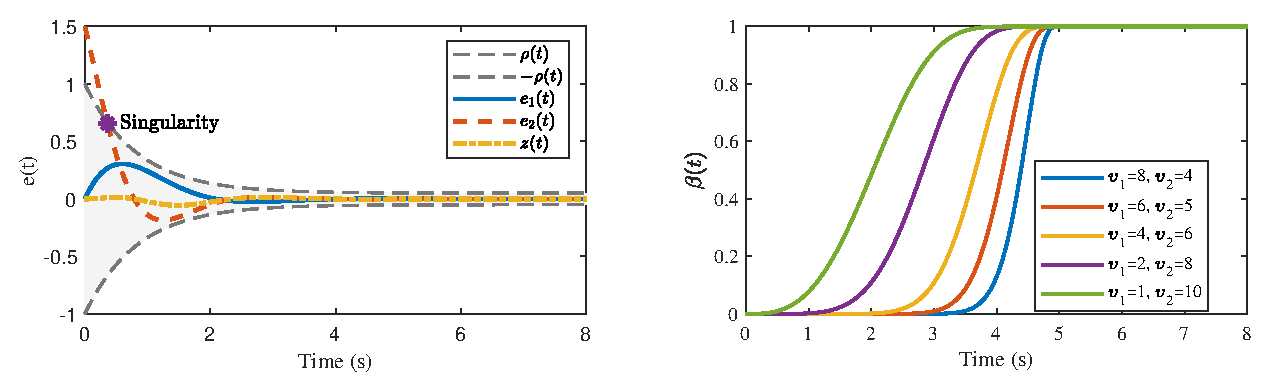
\includegraphics[width=0.9\textwidth]{fig1.eps}
	\caption{Error shift transformation and shift function.}
	\label{fig:1}
\end{figure}
\begin{remark}
	如 \cref{fig:1} 所示:左图给出了经移位变换后的缩放误差轨迹 $z(t)$ 相对于性能包络 $\rho(t)$ 的演化。即便存在 $|e(0)|>\rho(0)$ 的初值越界,由于 $\beta(0)=0$ 从而 $z(0)=0$,误差在变量层面被“强制合法化”,避免了传统 PPC 采用 $z=e/\rho$ 时在进入阶段出现的奇异性与可行域切换(往往需要投影算子或非对称放缩等权宜修补)。右图展示了不同形状参数 $(\upsilon_1,\upsilon_2)$ 下的 $\beta(t)$ 曲线族,体现出“前期更缓/更陡、后期更快/更慢”的可调缩放能力,可在力矩峰值与稳态精度之间进行显式权衡。综合来看,本文的 误差变换结构的特点在于:\textbf{(i)} 将预定义时间的边界收紧(Bernstein 加权的 $\rho$)与误差注入路径成形解耦成双调谐器,实现预定义时间+预设性能的可设计收敛路径;\textbf{(ii)} 通过 $z(0)=0$ 从源头消除初值奇异性与非法区问题,无需额外重置/投影机制;\textbf{(iii)} $\dot\rho(t),\dot\beta(t)$ 具备封闭、光滑、可界的解析形式,便于与饱和补偿、RBFNN 等模块级联并保持 Lyapunov 证明闭合.
	\end{remark}
	



\section{Main results}


This work presents a controller design methodology that integrates the backstepping approach with BLFs to achieve both predefined-time convergence and prescribed performance constraints. The structure of the proposed control algorithm is shown in \cref{fig:2}.
\begin{figure}[H]
	\centering
	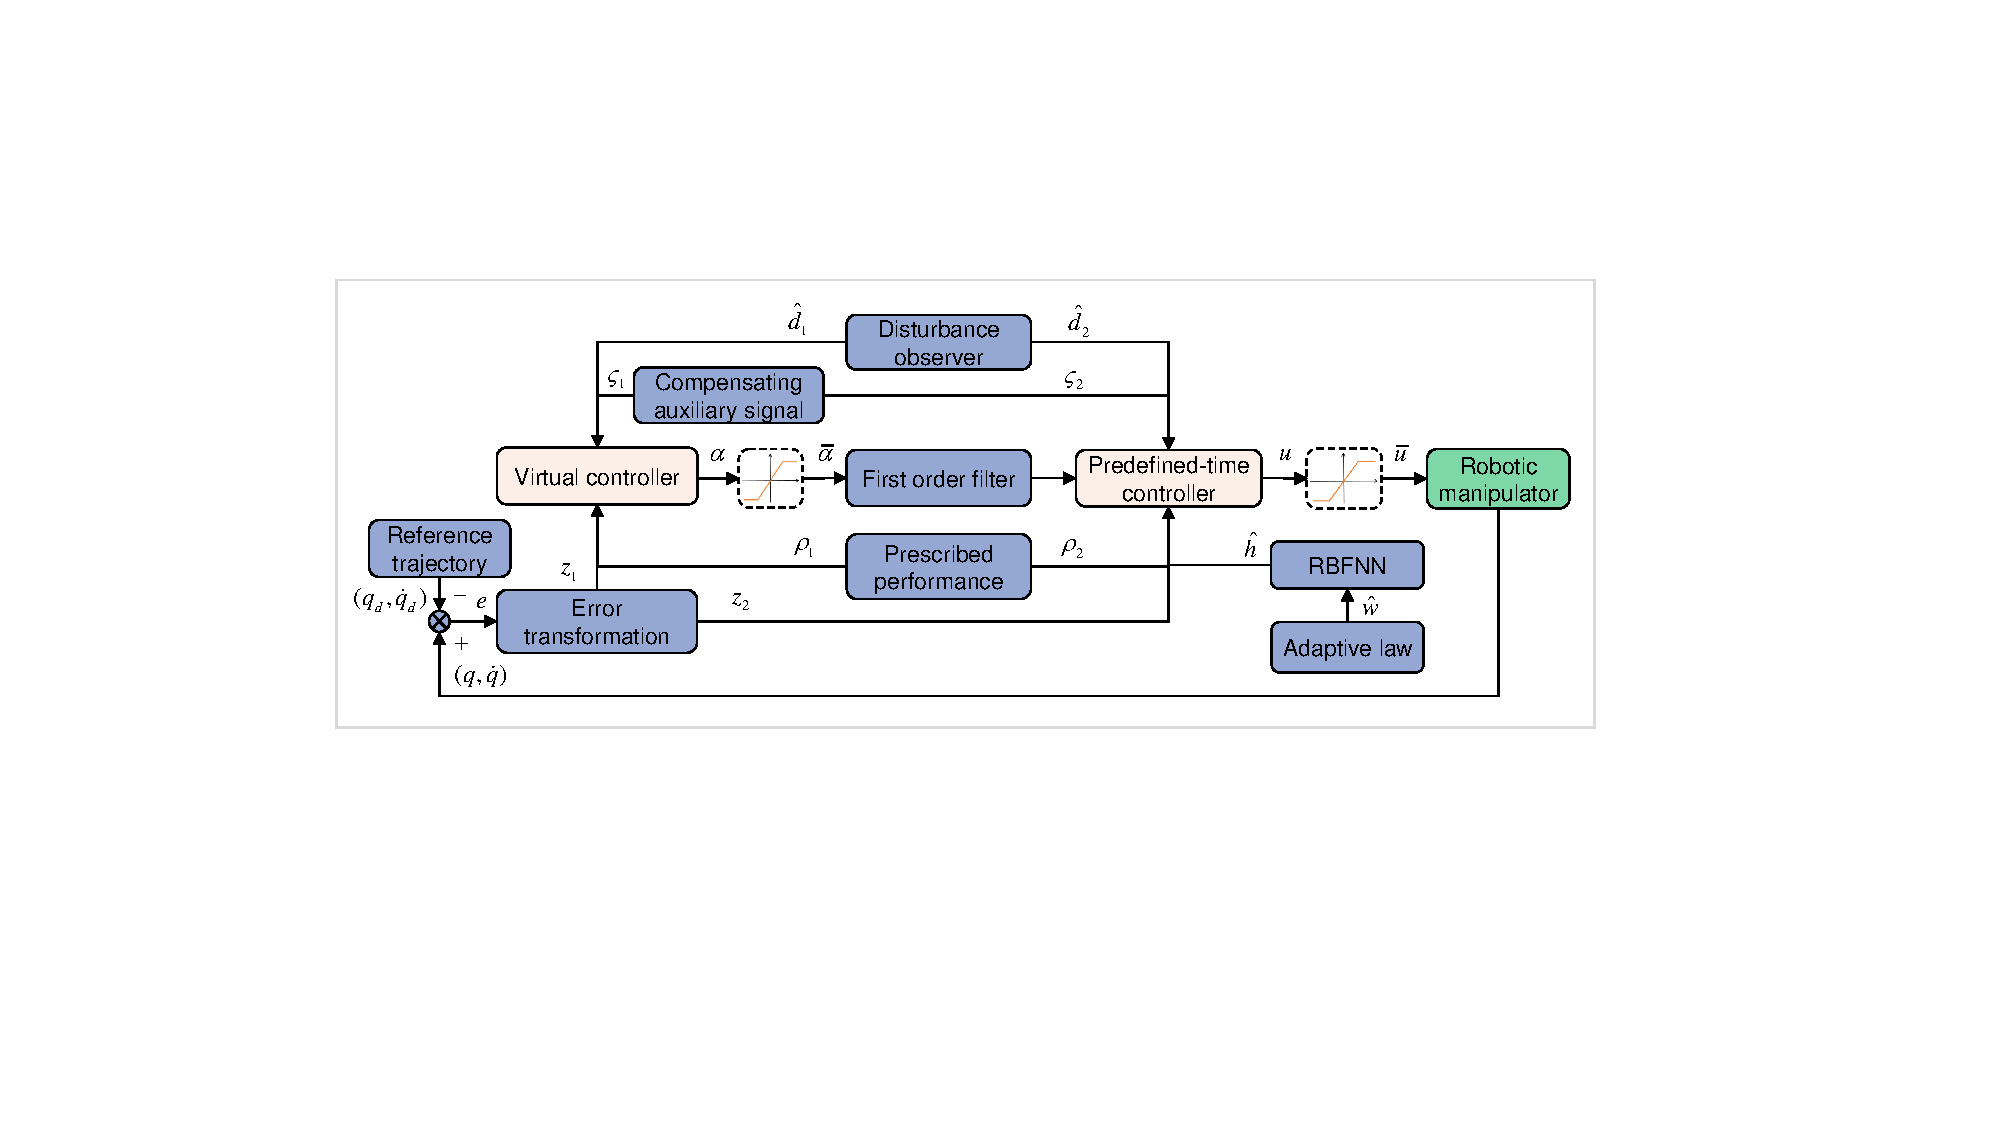
\includegraphics[width=0.9\textwidth]{fig2.pdf}
	\caption{The structure of the proposed controller}
	\label{fig:2}
\end{figure}



\par In a trajectory tracking control system, to  guarantee that tracking error meets the prescribed dynamic and steady-state performance requirements, define the tracking error as
\begin{subequations}\label{eq:20}
	\begin{align}
		&e_{1} = x_{1} - q_{d}, \\
	  &e_{2} = x_{2} -\alpha^{f}-\zeta,
	\end{align}
	\end{subequations}
	where $\alpha$ is the virtual control, $\bar{\alpha}$ denotes its elementwise saturation, $\alpha^{f}$ is a filtered version of $\bar{\alpha}$, and $\zeta_{1},\zeta \in\mathbb{R}^{n}$ are dynamic anti-saturation compensators of virtual and actual channels, respectively.
% where $\alpha^{f}$ is the filter output of $\bar{\alpha}$, $\bar{\alpha}$ 是$\alpha$的饱和后输出, $\alpha$ 是虚拟控制输入量. $\zeta_{i,1}, \zeta_{i,2}$ 分别为虚拟控制器和实际控制器的的抗饱和补偿量. 


\subsection{饱和补偿器构造}


为将饱和残差在预设时间 $T_\zeta<cT_p$($0<c<1$)内抽干,针对每个通道 $i$ 引入单通道动态补偿信号 $\zeta_{i}$,并选
\begin{equation}\label{eq:zeta2-pts}
\dot\zeta_i \ =\ \delta_i\ -\ \mu_2\,\zeta_i\ -\ g_i\,\Delta u_i,\quad
\delta_i\ =\ -\frac{\pi}{2\gamma T_\zeta}\Big(\mathrm{sig}(\zeta_i)^{\,1-\gamma}+\mathrm{sig}(\zeta_i)^{\,1+\gamma}\Big),
\end{equation}
其中 $0<\gamma<1,\ \mu_2>0$,$\zeta_i(0)=0$, $\mathrm{sig}(\zeta_i)^{1\pm \gamma}=|\zeta_i|^{1\pm \gamma}\mathrm{sig}(\zeta_i)$, 并取初值 $\zeta_{i}(0)=0$。



 To smooth the signal and facilitate the design of the subsequent control law, the filter of the virtual controller $\alpha^{f}$ is introduced with the following dynamic equations:
\begin{equation}\label{eq:22}
	\lambda \dot{\alpha}^{f}
	= -\left(\alpha^{f}-\alpha\right),
	\quad
	\alpha^{f}(0)=\alpha(0),
\end{equation}
where $0<\lambda<1$. Define the filtering error 
\begin{equation}\label{eq:23}
	\tilde{\alpha}= \alpha-\alpha^{f},
\end{equation}


\subsection{Controller design}


% 从而可在各 backstepping 级次精确定义虚拟/实际控制律,使 $\dot V\le -cV+\mu$ 并完成稳定性证明。

In the first step, a BLF is used as an energy function for the error dynamics. We choose:
\begin{equation}\label{eq:25}
	V_1= \frac{1}{2}\sum_{i=1}^{n} \frac{\rho_{i,1}^2 z_{i,1}^2}{\rho_{i,1}^2-z_{i,1}^2}. 
\end{equation}

求$V_1$ 的时间导数为
$$\dot z_{i,1}= e_{2} - \dot{q}_{d}+\alpha^{f}+\zeta$$
\begin{equation}\label{eq:25}
	\begin{aligned}
\dot V_1
&=\sum_{i=1}^{n}\left[
\frac{\rho_{i,1}^4\,z_{i,1}}{\big(\rho_{i,1}^{2}-z_{i,1}^{2}\big)^{2}}\;\dot z_{i,1}
\;-\;
\frac{\rho_{i,1}\,z_{i,1}^{4}}{\big(\rho_{i,1}^{2}-z_{i,1}^{2}\big)^{2}}\;\dot \rho_{i,1}
\right]\\
&=\sum_{i=1}^{n}\left[
\frac{\rho_{i,1}^4\,z_{i,1}}{\big(\rho_{i,1}^{2}-z_{i,1}^{2}\big)^{2}}(e_{2} -\dot{q}_{d}+\alpha^{f}+\zeta)
\;-\;
\frac{\rho_{i,1}\,z_{i,1}^{4}}{\big(\rho_{i,1}^{2}-z_{i,1}^{2}\big)^{2}}\;\dot \rho_{i,1}
\right]
\end{aligned}
\end{equation}




也可等价改写成提取公因子的形式:

\begin{equation}\label{eq:25}
	\begin{aligned}
\dot V_1
=\sum_{i=1}^{n}
\frac{\rho_{i,1}\,z_{i,1}}{\big(\rho_{i,1}^{2}-z_{i,1}^{2}\big)^{2}}
\Big(\rho_{i,1}^{3}(e_{2} -\dot{q}_{d}+\alpha^{f}+\zeta)-z_{i,1}^{3}\dot\rho_{i,1}\Big)\\
\end{aligned}
\end{equation}




记

$$
S_i \;\triangleq\;2V_{1,i}=\frac{\rho_{i,1}^2 z_{i,1}^2}{\rho_{i,1}^2-z_{i,1}^2},\qquad
G_i=\frac{\rho_{i,1}^4 z_{i,1}}{(\rho_{i,1}^2-z_{i,1}^2)^2},\quad
H_i=\frac{\rho_{i,1} z_{i,1}^4}{(\rho_{i,1}^2-z_{i,1}^2)^2}.
$$

$\dot z_{i,1}= e_{2,i}-\dot q_{d,i}+\alpha^{f}_i+\zeta_i$ 代入 BLF 导数后,经由
$\alpha^{f}_i=\alpha_i-\tilde\alpha_i$ 得到

$$
\dot V_1=\sum_i\!\Big[G_i e_{2,i}+G_i(\alpha_i+\zeta_i-\dot q_{d,i})-G_i\tilde\alpha_i-H_i\dot\rho_{i,1}\Big]
$$

选用标准 PTS 速度函数:

$$
\Psi_\eta(S)=\frac{\pi}{2\eta T_p}\Big(S^{\,1-\eta/2}+S^{\,1+\eta/2}\Big).
$$

将常数增益 $k_{1i}$ **改为状态依赖的 PTS 增益**:

$$
\boxed{
k_{1i}(z_{i,1},\rho_{i,1})
=\rho_{i,1}^2\;\frac{\Psi_\eta(S_i)}{S_i}
=\frac{\pi\,\rho_{i,1}^2}{2\eta T_p}\Big((2V_{1,i})^{-\eta/2}+(2V_{1,i})^{\eta/2}\Big).
}
$$

把它带回虚拟控制律:

$$
\boxed{
\alpha_i \;=\; \dot q_{d,i}-\zeta_i
-\;k_{1i}(z_{i,1},\rho_{i,1})\,
\frac{z_{i,1}(\rho_{i,1}^2-z_{i,1}^2)}{\rho_{i,1}^4}
+\;\frac{z_{i,1}^3}{\rho_{i,1}^3}\,\dot\rho_{i,1}.
}
$$

则一步 Lyapunov 导数化简为

$$
\boxed{
\dot V_1
= \sum_{i=1}^n \Big[
G_i e_{2,i}\;-\;\Psi_\eta(2V_{1,i})\;-\;G_i\tilde\alpha_i
\Big].
}
$$


In the second step, a BLF is used as an energy function for the error dynamics. We choose:
\begin{equation}\label{eq:25}
	V_2= \frac{1}{2}\sum_{i=1}^{n} \frac{\rho_{i,2}^2 z_{i,2}^2}{\rho_{i,2}^2-z_{i,2}^2}. 
\end{equation}




\subsubsection{BLF-based actual controller with DOB \& FLS (Step~2)}

\paragraph{Notation aligned with Step~1.}
For each channel $i=1,\dots,n$, keep
\[
z_{1,i}=e_{1,i}=x_{1,i}-q_{d,i},\qquad
z_{2,i}=e_{2,i}=x_{2,i}-\alpha_i^{f}-\zeta_i .
\]
The Step~1 BLF weights are
\[
G_{1,i}\;=\;\frac{\rho_{i,1}^4 z_{1,i}}{\bigl(\rho_{i,1}^{2}-z_{1,i}^{2}\bigr)^{2}},\quad
H_{1,i}\;=\;\frac{\rho_{i,1} z_{1,i}^{4}}{\bigl(\rho_{i,1}^{2}-z_{1,i}^{2}\bigr)^{2}},
\]
and the Step~2 BLF is
\[
V_2=\frac12\sum_{i=1}^{n}\frac{\rho_{i,2}^2 z_{2,i}^2}{\rho_{i,2}^2-z_{2,i}^2},
\]
with the corresponding weights
\[
P_i \;=\; \frac{\rho_{i,2}^4 z_{2,i}}{\bigl(\rho_{i,2}^{2}-z_{2,i}^{2}\bigr)^{2}},\qquad
H_{2,i}\;=\;\frac{\rho_{i,2} z_{2,i}^{4}}{\bigl(\rho_{i,2}^{2}-z_{2,i}^{2}\bigr)^{2}},\qquad
\Phi_{2,i}\;=\;\frac{z_{2,i}\bigl(\rho_{i,2}^{2}-z_{2,i}^{2}\bigr)}{\rho_{i,2}^{4}} .
\]
The G-PPF ${\rho}_{i,1}(t),{\rho}_{i,2}(t)$ and their derivatives $\dot\rho_{i,1}$, $\dot\rho_{i,2}$ follow \eqref{eq:gppf-def}–\eqref{eq:gppf-drho-post}.

\paragraph{Robot dynamics in acceleration form.}
From \eqref{eq:1}, the acceleration dynamics can be written as
\[
\dot x_2 = f_{\rm nom}(x)+\phi(x)+g(q)\,u_{\rm act}+d'(t),
\]
where $f_{\rm nom}(x)=-M^{-1}(q)\{C(q,\dot q)\,x_2+G(q)\}$,
$g(q)=M^{-1}(q)$, $\phi(x)$ collects structured uncertainties,
and $d'(t)$ collects external disturbances.
The applied input is $u_{\rm act}=M^{-1}(q)\bigl(\tau_{\rm act}-C(q,\dot q)x_2-G(q)\bigr)$ with $\tau_{\rm act}=\mathrm{sat}(\tau_{\rm cmd})$.

\paragraph{Time derivative of $V_2$.}
Using $\dot z_{2,i}=\dot x_{2,i}-\dot\alpha_i^{f}-\dot\zeta_i$, we obtain
\[
\dot V_2=\sum_{i=1}^n \Big[\,P_i\,\dot z_{2,i}-H_{2,i}\,\dot\rho_{i,2}\,\Big].
\]

\paragraph{Predefined-time shaping for Step~2.}
Define $S_{2,i}\triangleq 2V_{2,i}=\frac{\rho_{i,2}^2 z_{2,i}^2}{\rho_{i,2}^2-z_{2,i}^2}$ and
\[
\Psi_{\eta_2}(S)=\frac{\pi}{2\eta_2 T_p}\bigl(S^{\,1-\eta_2/2}+S^{\,1+\eta_2/2}\bigr),\quad 0<\eta_2<1.
\]
Choose the state-dependent gain
\begin{equation}\label{eq:k2-pts}
k_{2,i}(z_{2,i},\rho_{i,2})=\rho_{i,2}^{2}\,\frac{\Psi_{\eta_2}(S_{2,i})}{S_{2,i}}
=\frac{\pi\,\rho_{i,2}^2}{2\eta_2 T_p}\Big((2V_{2,i})^{-\eta_2/2}+(2V_{2,i})^{\eta_2/2}\Big).
\end{equation}

\paragraph{Fuzzy logic system (FLS) identifier.}
Let $\chi\in\mathbb{R}^m$ be the regressor and $\xi(\chi)\in\mathbb{R}^{N}$ the normalized basis
(see Sec.~\ref{sec:FLS}).
Approximate the structured uncertainty by
\[
\hat\phi_i(\chi)=\theta_i^\top \xi(\chi),
\]
with $\theta_i\in\mathbb{R}^{N}$ adapted online by
\begin{equation}\label{eq:theta-law}
\dot\theta_i = \kappa_i\,P_i\,z_{2,i}\,\xi(\chi) \;-\; \sigma_i\,\theta_i,\qquad
\kappa_i>0,\ \sigma_i\ge 0 .
\end{equation}

\paragraph{Disturbance observer (DOB).}
Using a first-order filter for $\dot x_2$,
\[
\dot\eta=-\omega_d\,\eta+\omega_d\,x_2,\qquad \hat{\dot x}_2=\omega_d(x_2-\eta),
\]
the DOB estimating the residual disturbance is
\begin{equation}\label{eq:dob}
\dot{\hat d}= -\Lambda_o\,\hat d
+\Lambda_o\Big(\hat{\dot x}_2 - f_{\rm nom}(x) - g(q)\,u_{\rm act} - \hat\phi(\chi)\Big),
\quad \Lambda_o=\mathrm{diag}\{\lambda_{o,i}\}>0,
\end{equation}
where $u_{\rm act}$ uses the saturated torque $\tau_{\rm act}$ (not the command).

\paragraph{Actual controller (Step~2).}
Let $G_{1,i}$ be the Step~1 weight above and define $G_1=\mathrm{col}\{G_{1,i}\}$,
$P=\mathrm{col}\{P_i\}$,
$\Phi_2=\mathrm{col}\{\Phi_{2,i}\}$.
The torque command is designed as
\begin{equation}\label{eq:tau-cmd}
\boxed{
\begin{aligned}
\tau_{\rm cmd} &= C(q,\dot q)\,x_2 + G(q) \\
&\quad + M(q)\Big[
\dot\alpha^{f}+\dot\zeta
\;-\;\mathrm{diag}(G_1./P)\,z_{2}
\;-\;k_{2}(z_{2},\rho_{2})\odot \Phi_{2}
\;+\;\Big(\tfrac{z_{2}^{\odot 3}}{\rho_{2}^{\odot 3}}\Big)\odot \dot\rho_{2} \\
&\hspace{24mm}
\;-\;\hat\phi(\chi)
\;-\;\hat d
\;-\;k_s\,\mathrm{sat}\!\big(z_{2}/\phi\big)
\Big],
\end{aligned}}
\end{equation}
where all vector products are elementwise, ``./'' is elementwise division,
$k_s>0$ is a robustifying gain and $\phi>0$ a saturation width. The applied torque is
$\tau_{\rm act}=\mathrm{sat}(\tau_{\rm cmd})$, and $\zeta$ follows \eqref{eq:zeta2-pts}.

\paragraph{Closed-loop analysis sketch.}
Adding $\dot V_1$ (Step~1 result) and $\dot V_2$, and substituting \eqref{eq:tau-cmd}–\eqref{eq:dob} and
\eqref{eq:theta-law}, we obtain the cancellations
\[
P_i\!\left(-\tfrac{G_{1,i}}{P_i}z_{2,i}\right)=-G_{1,i}z_{2,i},\qquad
P_i\!\left(\tfrac{z_{2,i}^3}{\rho_{i,2}^3}\dot\rho_{i,2}\right)=H_{2,i}\dot\rho_{i,2},
\]
so that
\[
\dot V_1+\dot V_2
\;\le\;
-\sum_{i=1}^n \Psi_{\eta_1}(2V_{1,i})
-\sum_{i=1}^n \Psi_{\eta_2}(2V_{2,i})
-\sum_{i=1}^n k_s\,|P_i|\,\Big\|\mathrm{sat}\big(z_{2,i}/\phi\big)\Big\|_1
-\frac{1}{\lambda}\tilde\alpha^\top C\,\tilde\alpha
-\frac{\lambda_{o,\min}}{\gamma_o}\|\tilde d\|^2,
\]
where $\tilde\alpha=\alpha-\alpha^f$, $\tilde d=\hat d-d'$, and the FLS term is canceled by the quadratic term
$\frac{1}{2\kappa_i}\tilde\theta_i^\top\tilde\theta_i$ under \eqref{eq:theta-law}.
With the G-PPF properties and bounded initial conditions, the closed loop is
predefined-time stable (zero input) and PTS–ISS under bounded disturbances.





% where $ \omega_j>0$ is an adaptive gain. Its adaptation law is
% \begin{equation}\label{eq:26}
% \dot{\omega}_j=\begin{cases}
% -\vartheta V_j,& \omega_{\min}<\omega_{j}<\omega_{\max},\\
% \max(0,-\vartheta V_j),& \omega_{j}= \omega_{\min},\\
% \min(0,-\vartheta V_j),& \omega_{j}= \omega_{\max},
% \end{cases}
% \end{equation}
% with $\vartheta>0$, $ 0 < \omega_{\min} \le \omega_{j} \le \omega_{\max}$.

% \begin{remark}
% 	由自适应律\cref{eq:26}可知,$\omega_{j}$ 始终受投影算子约束而保持正数有界,且单调非增。在大误差阶段加重屏障惩罚、误差减小时自动降权,比固定权重 BLF 更执行器友好,并便于与预定义时间项配平。
% \end{remark}
% The time derivation of $V_1$ yields 
% % \begin{equation}
% % 	\dot{V}_{1} = \sum_{i=1}^{n} \left[ \frac{z_{i,1} \dot{z}_{i,1}}{\rho_{i,1}^{2} - z_{i,1}^{2}} - \frac{\dot{\rho}_{i,1}}{\rho_{i,1}} \frac{z_{i,1}^{2}}{\rho_{i,1}^{2} - z_{i,1}^{2}} \right]
% % 	\label{eq:V1}
% % 	\end{equation}

% 	\begin{equation}\label{eq:27}
% 	\dot{V}_{1}=-\frac{\dot{\omega}_{1}}{2 \omega_{1}^{2}}\sum_{i=1}^{n}\ln \frac{\rho_{i,1}^{2}}{\rho_{i,1}^{2}-z_{i,1}^{2}}+\frac{1}{\omega_{1}} \sum_{i=1}^{n} \left[ \frac{z_{i,1} \dot{z}_{i,1}}{\rho_{i,1}^{2} - z_{i,1}^{2}} - \frac{\dot{\rho}_{i,1}}{\rho_{i,1}} \frac{z_{i,1}^{2}}{\rho_{i,1}^{2} - z_{i,1}^{2}} \right].
% 	\end{equation}

% 	According to \cref{eq:19,eq:20}, one has
% 	\begin{equation}	\label{eq:28}
% 	\dot{z}_{i,1} = \dot{\beta} e_{i,1} + \beta \dot{e}_{i,1}=\dot{\beta} e_{i,1} + \beta (e_{i,2}-\dot q_{i,d}+\alpha_{i}-\delta_{i,1}+\mu_1 \zeta_{i,1}),
% 	\end{equation}

% 	Substituting \cref{eq:28} into \cref{eq:27}, and letting $\varGamma_{i,1} = {z_{i,1}}/({\rho_{i,1}^2 - z_{i,1}^2})$, we have
% 	\begin{equation}	\label{eq:29}
% 			\begin{aligned}
% 			\dot{V}_{1} &= -\frac{\dot{\omega}_{1}}{2 \omega_{1}^{2}}\sum_{i=1}^{n}\ln\frac{\rho_{i,1}^{2}}{\rho_{i,1}^{2}-z_{i,1}^{2}}+\frac{1}{\omega_{1}}\sum_{i=1}^{n} \left[ \frac{z_{i,1} (\dot{\beta} e_{i,1} + \beta \dot{e}_{i,1})}{\rho_{i,1}^{2} - z_{i,1}^{2}} - \frac{\dot{\rho}_{i,1}}{\rho_{i,1}} \frac{z_{i,1}^{2}}{\rho_{i,1}^{2} - z_{i,1}^{2}} \right] \\
% 			% &=-\frac{\dot{\omega}_{1}}{2 \omega_{1}^{2}}\sum_{i=1}^{n}\frac{z_{i,1}^{2}}{\rho_{i,1}^{2}-z_{i,1}^{2}}+\frac{1}{\omega_{1}}\sum_{i=1}^{n} \frac{\dot{\beta} e_{i,1} z_{i,1}}{\rho_{i,1}^{2} - z_{i,1}^{2}} +\frac{1}{\omega_{1}}\sum_{i=1}^{n} \varGamma_{i,1} \left[\beta \left(e_{i,2}-\dot q_{i,d}+\alpha_{i}-\delta_{i,1}+\mu_1 \zeta_{i,1}- \frac{\dot{\rho}_{i,1}e_{i,1}}{\rho_{i,1}}\right)  \right]\\
% 			&=-\frac{\dot{\omega}_{1}}{2 \omega_{1}^{2}}\sum_{i=1}^{n}\frac{z_{i,1}^{2}}{\rho_{i,1}^{2}-z_{i,1}^{2}}+\frac{\varGamma_{i,1}}{\omega_{1}}\sum_{i=1}^{n} \left[\dot{\beta} e_{i,1}+\beta \left(e_{i,2}-\dot q_{i,d}+\alpha_{i}-\delta_{i,1}+\mu_1 \zeta_{i,1}- \frac{\dot{\rho}_{i,1}}{\rho_{i,1}}e_{i,1}\right)  \right],
% 		\end{aligned}
% 			\end{equation}

% To suppress the system error and achieve performance convergence, the virtual control law $\alpha_i$ is designed as 
% \begin{equation}	\label{eq:30}
% 	\begin{aligned}
% 	\alpha_i
% 	% &= \dot q_{i,d}-e_{i,2}+\delta_{i,1}-\mu_1 \zeta_{i,1}+\frac{\dot{\omega}_{1}e_{i,1}}{2 \omega_{1}}-\frac{\iota_1  \dot{\beta}^{2} e_{i,1}^{3} }{\rho_{i,1}^{2} - z_{i,1}^{2}} 
% 	% +\frac{\dot\rho_{i,1}}{\rho_{i,1}} e_{i,1}- k_{i,1} e_{i,1}
% 	% - \omega_{1} e_{i,1} \Psi_{i,1}-{\hat d}_{i,1}\\
% 	&= \dot q_{i,d}-e_{i,2}+\delta_{i,1}-\mu_1 \zeta_{i,1}+e_{i,1}\left( \frac{\dot{\omega}_{1}}{2 \omega_{1}}-\frac{\iota_1  \dot{\beta}^{2} e_{i,1}^{2} }{\rho_{i,1}^{2} - z_{i,1}^{2}} 
% 	+\frac{\dot\rho_{i,1}}{\rho_{i,1}} - k_{i,1} 
% 	- \omega_{1} \Psi_{i,1}   \right)-{\hat d}_{i,1}
% \end{aligned}
% \end{equation}
% where, $k_{1}=\text{diag}(k_{1,1}, k_{2,1},\cdots, k_{n,1})$, $k_{i,1}>0 $, $\iota_2$, $\Psi_{i,1}={\pi}/({2 \eta\,T_p})[1+(n z_{i,1}\varGamma_{i,1}/2)^{{\eta}/{2}}]$ is a regulation term associated with a predefined-time and performance function to achieve convergence regulation of the error. \(\hat d_{i,1}\) is a disturbance estimate.
% Introduce the composite error and the first-order sliding disturbance observer:
% \begin{equation}\label{eq:31}
% 	 s_{i,1} = e_{i,2} + v_{i,1} e_{i,1}, \quad v_{i,1}>0,
% \end{equation}
% % 其中$v_{i,1}>0$。
% % 为了抑制硬切换引起的抖振,设计如下饱和函数:
% %  \begin{equation}\label{eq:33}
% %       \operatorname{sat}(s_i)   
% %       = 
% %       \begin{cases}  
% %         1, & s_i>\sigma_i,\\
% % 		 s_i/\sigma_i, & |s_i| \le \sigma_i,\\     
% %       -1, &s_i<-\sigma_i.
% %       \end{cases}
% % \end{equation}
% % 其中$\sigma_i>0$. 
% % 引入一个Super-Twisting观测器来在线估计并补偿系统的不确定扰动。构造复合误差如下:
% % 为实现扰动估计,引入辅助信号$\xi_{i,1}$, \(\hat d_{i,1}\)的动态方程如下
% %  \begin{equation}\label{eq:32}
% %       \dot{\hat d}_{i,1} = -\hbar_{i,1} |s_{i,1} \vert^{\frac{1}{2}} \operatorname{sgn}(s_{i,1})+\xi_{i,1}, 
% % \end{equation}
% % \begin{equation}\label{eq:32}
% %  \dot{\xi}_{i,1} = -\hbar_{i,2} \operatorname{sgn}(s_{i,1}),
% % \end{equation}
% % 其中$\hbar_{i,1} , \hbar_{i,2} >\bar{d}$. 定义估计误差为$\tilde{d}_{i,1} = d_{i,1} - \hat{d}_{i,1}$, $\dot{\tilde{d}}_{i,1} = \hbar_{i,1}\left| s_{i,1} \right|^{\frac{1}{2}} \operatorname{sgn}(s_{i,1}) - \xi_{i,1} + \dot{d}_{i.1}$.


% % 为了抑制硬切换引起的抖振,设计如下饱和函数:
% %  \begin{equation}\label{eq:33}
% %       \operatorname{sat}(s_i)   
% %       = 
% %       \begin{cases}  
% %         1, & s_i>\sigma_i,\\
% % 		 s_i/\sigma_i, & |s_i| \le \sigma_i,\\     
% %       -1, &s_i<-\sigma_i.
% %       \end{cases}
% % \end{equation}
% % 其中$\sigma_i>0$. 
% % 将扰动估计量\(\hat d_i\)表示为
% %  \begin{equation}\label{eq:32}
% %       \dot{\hat d}_{i,1} = -\hbar_{i,1} \operatorname{sat}(s_i).
% % \end{equation}
% %   其中$\hbar_{i,1} >\bar{d}$.
 
% % \(\hat d_{i,1} \)的动态方程设计如下
% \begin{equation}\label{eq:32}
%       \dot{\hat d}_{i,1} = -\hbar_{i,1} \operatorname{sgn}(s_{i,1})-\varpi_{i,1} {\hat d}_{i,1}+\hbar_{i,1}\frac{\varGamma_{i,1}}{{\omega}_{1}},
% \end{equation}
% where $\hbar_{i,1} >\bar{d}, \varpi_{i,1}>\hbar_{i,1}+1$, and $\tilde{d}_{i,1} = d_{i,1} - \hat{d}_{i,1}$.

% Since \cref{eq:26}, $\dot{\omega}_{j} \leq 0$, one has $-\dot{\omega}_{j}/(2 \omega_{j}^{2}) \geq 0$. Let $\iota_j>0$ Using \cref{lemma:4} and Young's inequality gives
% 		\begin{equation}\label{eq:33}
% -\frac{\dot{\omega}_{j}}{2 \omega_{j}^{2}}\sum_{i=1}^{n}\ln\frac{\rho_{i,j}^{2}}{\rho_{i,j}^{2}-z_{i,j}^{2}}
% \leq -\frac{\dot{\omega}_{j}}{2 \omega_{j}^{2}}\sum_{i=1}^{n}\frac{z_{i,j}^{2}}{\rho_{i,j}^{2}-z_{i,j}^{2}},
% 	\end{equation}
% 		\begin{equation}\label{eq:34}
% 			\sum_{i=1}^{n} \frac{\dot{\beta} e_{i,j} z_{i,j}}{\rho_{i,j}^{2} - z_{i,j}^{2}} 
% 			\leq 
% 			 \sum_{i=1}^{n} \frac{\iota_j  \dot{\beta}^{2} e_{i,j}^{2} z_{i,j}^{2}}{(\rho_{i,j}^{2} - z_{i,j}^{2})^{2}} 
% 			+ \frac{n}{4\iota_j}.
% 			\end{equation}
			
% % From \cref{lemma:1}, letting $\mathcal{X} =1/2\sum_{i=1}^{n} \ln({\rho_{j}^2}/{\rho_{j}^2-e_{i,j}^2}), \mathcal{Y} =1, \mathcal{Z}_{1}= {1-{\eta}/{2}}, \mathcal{Z}_{2}={\eta}/{2}, \mathcal{Z}_{3}= (\eta/2)^{(\eta/(2-\eta))}$, we have
% % \begin{equation}\label{eq:37}
% % 	\left(\frac{1}{2}\sum_{i=1}^{n} \ln\frac{\rho_{j}^2}{\rho_{j}^2-e_{i,j}^2}\right)^{1-\frac{\eta}{2}} \le \frac{1}{2} \sum_{i=1}^{n} \ln\frac{\rho_{j}^2}{\rho_{j}^2-e_{i,j}^2}+\left( 1-\frac{\eta}{2}\right) \left(\frac{\eta}{2}\right)^{\frac{\eta}{2-\eta}}.
% % \end{equation}

% Furthermore, substituting \cref{eq:30,eq:33,eq:34} into \cref{eq:29}, we obtain
% % \begin{equation}\label{eq:38}
% % 	\begin{aligned}
% % 	\dot{V}_{1} 
% % 	&\le\sum_{i=1}^{n} \varGamma_{i,1} \frac{1}{\omega_{1}}\left[-\frac{\dot{\omega}_{1}z_{i,1}}{2 \omega_{1}}+\frac{\iota_1  \dot{\beta}^{2} e_{i,1}^{2} z_{i,1}}{\rho_{i,1}^{2} - z_{i,1}^{2}}  + \beta  \left(e_{i,2}-\dot q_{i,d}+\alpha_{i}-\delta_{i,1}-\mu_1 \zeta_{i,1}- \frac{\dot{\rho}_{i,1} e_{i,1}}{\rho_{i,1}}\right)  \right] + \frac{1}{4 \omega_{1} \iota_1 }
% % 	\\
% % 	&\le\sum_{i=1}^{n} \varGamma_{i,1} \left[ \frac{\beta}{\omega_{1}} \left(-\frac{\dot{\omega}_{1}e_{i,1}}{2 \omega_{1}}+\frac{\iota_1  \dot{\beta}^{2} e_{i,1}^{3}}{\rho_{i,1}^{2} - z_{i,1}^{2}}+e_{i,2}-\dot q_{i,d}+\alpha_{i}-\delta_{i,1}-\mu_1 \zeta_{i,1}- \frac{\dot{\rho}_{i,1} e_{i,1}}{\rho_{i,1}}\right) \right] + \frac{1}{4 \omega_{1} \iota_1 },
% % \end{aligned}
% % 	\end{equation}

% % 进一步, From \cref{eq:30,eq:38}, 我们得到
% \begin{equation}\label{eq:35}
% 	\begin{aligned}
% 		\dot{V}_{1}
% 		 & \le - \sum_{i=1}^{n}\varGamma_{i,1}z_{i,1}\Psi_{i,1}  - \frac{1}{\omega_{1}}\sum_{i=1}^{n} \left(\frac{k_{i,1} z_{i,1}^2}{\rho_{i,1}^2 - z_{i,1}^2}-  \frac{ z_{i,1}\hat d_{i,1}}{\rho_{i,1}^2 - z_{i,1}^2}\right) + \frac{n}{4  \omega_{1} \iota_1 }.                           
% 	\end{aligned}
% \end{equation}
% % \begin{equation}\label{eq:23}
% % 	\begin{aligned}
% % 		\dot{V}_{1}
% % 		 & = - \sum_{i=1}^{n}\varGamma_{i,1}z_{i,1}\left[\frac{\pi}{\eta\,T_p}\,
% % 	\left( 2^{-1}
% % 	+
% % 	n^{\frac\eta2} 2^{-\tfrac\eta2 -1}\,\left(\frac{z_{i,1}^2}{\rho_{i,1}^2 - z_{i,1}^2}\right)^{\frac{\eta}{2}}\right)  \right]                             \\
% % 		 & -\frac{\beta}{\omega}\sum_{i=1}^{n}\frac{ z_{i,1}{\tilde{\alpha}}}{\rho_{i,1}^{2}-z_{i,1}^{2}}- \sum_{i=1}^{n}k_{i,1} \frac{z_{i,1}^2}{\rho_{i,1}^2 - z_{i,1}^2}- \sum_{i=1}^{n}k_{i,\sigma} \frac{ z_{i,1}\sigma_{i,1}}{\rho_{i,1}^2 - z_{i,1}^2}+ \frac{1}{4  \omega \iota_1 } ,                            
% % 	\end{aligned}
% % \end{equation}


% The second level BLF candidates are chosen as
% \begin{equation}	\label{eq:36}
% 	V_2=V_1+\frac{1}{2 \omega_2}\sum_{i=1}^{n} \ln\frac{\rho_{i,2}^2}{\rho_{i,2}^2-z_{i,2}^2}, 
% \end{equation}

% The time derivation of $V_2$ yields
% \begin{equation}\label{eq:37}
% 	\dot{V}_{2} = \dot{V}_{1}-\frac{\dot{\omega}_{2}}{2 \omega_{2}^{2}}\sum_{i=1}^{n}\ln\left(\frac{\rho_{i,2}^{2}}{\rho_{i,2}^{2}-z_{i,2}^{2}}\right)+\frac{1}{\omega_{2}}\sum_{i=1}^{n} \left[ \frac{z_{i,2} \dot{z}_{i,2}}{\rho_{i,2}^{2} - z_{i,2}^{2}} - \frac{\dot{\rho}_{i,2}}{\rho_{i,2}} \frac{z_{i,2}^{2}}{\rho_{i,2}^{2} - z_{i,2}^{2}} \right].
% 	\end{equation}
	
% From \cref{eq:2,eq:19,eq:20}, one has 
% 	\begin{equation}\label{eq:38}
% 		\begin{aligned}
% 	\dot{z}_{i,2} =& \dot{\beta} e_{i,2} + \beta \dot{e}_{i,2}
% 	 =\dot{\beta} e_{i,2} + \beta \left(f_i + g_i u_i + h_i-\dot{\alpha}^{f}_{i}-\delta_{i,2}+\mu_2 \zeta_{i,2}\right).
% \end{aligned}
% 	\end{equation}

% Substituting \cref{eq:38} into \cref{eq:37}, and letting $\varGamma_{{i,2}}  ={z_{i,2}}/({\rho_{{i,2}}^2 - z_{i,2}^2})$ gives
% \begin{equation}\label{eq:39}
% 	\begin{aligned}
% 		\dot V_2
% 		%  & =
% 		% \dot{V}_{1} -\frac{\dot{\omega}_{2}}{2 \omega_{2}^{2}}\sum_{i=1}^{n}\ln\left(\frac{\rho_{i,2}^{2}}{\rho_{i,2}^{2}-z_{i,2}^{2}}\right)+\frac{1}{\omega_{2}}\sum_{i=1}^n \varGamma_{{i,2}} \left[\dot{\beta} e_{i,2} + \beta \left(f_i + g_i u_i + h_i-\dot{\alpha}^{f}_{i}-\delta_{i,2}+\mu_2 \zeta_{i,2}-\frac{e_{i,2}\dot{\rho}_{i,2}}{\rho_{{i,2}}}\right)\right]\\
% 		%  & =\dot{V}_{1}+ \sum_{i=1}^n \varGamma_{{i,2}} \frac{\beta}{\omega_{2}} \left(-\frac{\dot{\omega}_{2} e_{i,2}}{2 \omega_{2}}+f_i + g_i u_i + h_i-\dot{\alpha}^{f}_{i}-\delta_{i,2} +\mu_2 \zeta_{i,2} +\frac{\iota_2  \dot{\beta}^{2} e_{i,2}^{3}}{\rho_{i,1}^{2} - e_{i,2}^{2}}-\frac{e_{i,2}\dot{\rho}_{i,2}}{\rho_{{i,2}}} \right)+\frac{1}{4 \omega_{2}\iota_2}\\
% 		 & =\dot{V}_{1}+ \sum_{i=1}^n \frac{\beta}{\omega_{2}} \varGamma_{{i,2}}  \left[f_i + g_i u_i + h_i-\dot{\alpha}^{f}_{i}-\delta_{i,2} +\mu_2 \zeta_{i,2} +e_{i,2}\left(\frac{\iota_2  \dot{\beta}^{2} e_{i,2}^{2}}{\rho_{i,1}^{2} - z_{i,2}^{2}} -\frac{\dot{\omega}_{2}}{2 \omega_{2}}  -\frac{\dot{\rho}_{i,2}}{\rho_{{i,2}}}\right) \right]+\frac{n}{4 \omega_{2} \iota_2},
% 	\end{aligned}
% \end{equation}


% Further, to enforce performance and cancel unknown terms we design the main control law as
% \begin{equation}\label{eq:40}
% 	u_i = g_i^{-1}\left[-\,f_i - \hat{h}_i + \dot{\alpha}^{f}_{i}+\delta_{i,2}-\mu_2 \zeta_{i,2}+e_{i,2}\left(-\frac{\iota_2  \dot{\beta}^{2} e_{i,2}^{2}}{\rho_{i,1}^{2} - z_{i,2}^{2}} +\frac{\dot{\omega}_{2}}{2 \omega_{2}}+\frac{\dot{\rho}_{i,2}}{\rho_{{i,2}}}- k_{i,2}- \omega_{2}\Psi_{{i,2}}   \right)-\hat d_{i,2}
% 	\right],
% \end{equation}
% % \begin{equation}\label{eq:26}
% % 	u = Cx_2 + G + M \left[\,
% % 	- \hat{h} \operatorname{sgn}(e_{2}) + \dot{\alpha}^{f}
% % 	- \frac{e_{2}\dot{\rho_{2}}}{\rho_{2}}- k_{2}e_{2}
% % 	- e_{2} \Psi_{2}
% % 	\right],
% % \end{equation}
% where $k_{2}=\text{diag}(k_{1,2}, k_{2,2},\cdots, k_{n,2})$, $k_{i,2}>0 $, $\iota_2$, $ \Psi_{i,2}={\pi}/({2 \eta\,T_p})
% 	[1+(n z_{i,2}\varGamma_{i,2}/2)^{{\eta}/{2}}]$.
	
% The unknown dynamics is approximated online by an RBFNN,
% $\hat h_i=\hat w_i^{\top}Q_i(\chi)$ with input $\chi=[x_{i,1},x_{i,2}]^\top$.
% The weight adaptation is chosen as
% \begin{equation}\label{eq:42}
% 	\dot{\hat w}_i
% 	=\frac{\beta }{\omega_{2}} \varrho_i\, Q_i\, \varGamma_{{i,2}} - \kappa_i \,\hat w_i,
% \end{equation}
% with learning rate $\varrho_i>0$ and leakage $\kappa_i>0$.

% For disturbance rejection, define the composite sliding signal
% $s_{i,2}=e_{i,2}+v_{i,2}e_{i,1}$ ($v_{i,2}>0$) and employ
% \begin{equation}\label{eq:41}
% 	\dot{\hat d}_{i,2} = -\hbar_{i,2} \operatorname{sgn}(s_{i,2})-\varpi_{i,2} {\hat d}_{i,2}+\hbar_{i,2} \frac{ \varGamma_{{i,2}}}{{\omega}_{1}},
% \end{equation}
% where $\hbar_{i,2} >\bar{d}, \varpi_{i,2}>\hbar_{i,2}+1$, and $\tilde{d}_{i,2} = d_{i,2} - \hat{d}_{i,2}$.
% % 构造滑模面如下:
% % \begin{equation}\label{eq:41}
% % 	 s_{i,2} = y_{i,2} + v_{i,2} y_{i,1}, 
% % \end{equation}
% % 其中$y_{i,1}, y_{i,2}$定义如下:
% % \begin{equation}\label{eq:46}
% % y_{i,1}=\dot q_i -\alpha_{i,\mathrm{sat}},
% % \quad
% % y_{2,i}=\ddot q_i-\dot{\tilde\alpha}_i.
% % \end{equation}


%   % 扰动估计量\(\hat d_{i,2}\)表示为
% %  \begin{equation}\label{eq:47}
% %       \dot{\hat d}_{i,2} = -k_{d,2}\operatorname{sgn}(s_{i,2}).
% % \end{equation}
% % 其中$k_{d,2}>\bar{d}$.
% % 为实现扰动估计,引入辅助信号$\xi_{i,2} $, \(\hat d_{i,2} \)的动态方程如下
% %  \begin{equation}\label{eq:32}
% %       \dot{\hat d}_{i,2}  = -\varpi_{i,1}  |s_{i,2}  \vert^{\frac{1}{2}} \operatorname{sgn}(s_{i,2} )+\xi_{i,2} , 
% % \end{equation}
% % \begin{equation}\label{eq:32}
% %  \dot{\xi}_{i,2}  = -\varpi_{i,2} \operatorname{sgn}(s_{i,2} ),
% % \end{equation}
% % 其中$\varpi_{i,1}, \varpi_{i,2} >\bar{d}$. 定义估计误差为$\tilde{d}_{i,2}  = d_{i,2}  - \hat{d}_{i,2} $, $\dot{\tilde{d}}_{i,2}  = \varpi_{i,1}\left| s_{i,2}  \right|^{\frac{1}{2}} \operatorname{sgn}(s_{i,2} ) - \xi_{i,2} + \dot{d}_{i,2}$.


% % 令$s_{i} = \frac{e_{{i,2}}}{\rho_{{i,2}}^2 - e_{{i,2}}^2}$


% % According to Young's inequality, we have
% % \begin{equation}\label{eq:43}
% % 		\sum_{i=1}^{n} \frac{\dot{\beta} e_{i,2} z_{i,2}}{\rho_{i,1}^{2} - z_{i,2}^{2}} 
% % 		\leq 
% % 		 \sum_{i=1}^{n} \frac{\iota_2  \dot{\beta}^{2} e_{i,2}^{2} z_{i,2}^{2}}{(\rho_{i,1}^{2} - z_{i,2}^{2})^{2}} 
% % 		+ \frac{n}{4\iota_2 }.
% % \end{equation}
% % From \cref{eq:43,eq:49}, we can obtain
% % \begin{equation}\label{eq:50}
% % 	\begin{aligned}
% % 		\dot V_2
% % 		 & \le \dot{V}_{1}+ \sum_{i=1}^n \varGamma_{{i,2}} \frac{\beta}{\omega_{2}} \left(-\frac{\dot{\omega}_{2} e_{i,2}}{2 \omega_{2}}+f_i + g_i u_i + h_i+\dot{\alpha}^{f}_{i}-\delta_{i,2} -\mu_2 \zeta_{i,2} +\frac{\iota_2  \dot{\beta}^{2} e_{i,2}^{3}}{\rho_{i,1}^{2} - e_{i,2}^{2}}-\frac{e_{i,2}\dot{\rho}_{i,2}}{\rho_{{i,2}}} \right)+\frac{1}{4\iota_2},
% % 	\end{aligned}
% % \end{equation}

% From \cref{eq:33,eq:34,eq:35}, and substituting the control law \cref{eq:40} into \cref{eq:39}, we get
% \begin{equation}\label{eq:44}
% 	\begin{aligned}
% 		\dot{V}_{2}
% 		& = - \sum_{i=1}^{n}\varGamma_{i,1}z_{i,1}\Psi_{i,1}  - \frac{1}{\omega_{1}}\sum_{i=1}^{n}\frac{k_{i,1} z_{i,1}^2}{\rho_{i,1}^2 - z_{i,1}^2}- \frac{1}{\omega_{1}}\sum_{i=1}^{n} \frac{ z_{i,1}\hat d_{i,1}}{\rho_{i,1}^2 - z_{i,1}^2} \\
% 		 & - \sum_{i=1}^{n}\varGamma_{i,2}z_{i,2}\Psi_{i,2} - \frac{1}{\omega_{2}}\sum_{i=1}^{n}\frac{ k_{2,i} z_{i,2}^2}{\rho_{2i}^2 - e_{i,2}^2}  + \frac{\beta }{\omega_{2}}\sum_{i=1}^{n} \varGamma_{i,2} (h_{i}-\hat{h}_{i})  \\
% 		 &- \frac{1}{\omega_{2}}\sum_{i=1}^{n} \frac{ z_{i,2}\hat d_{i,2}}{\rho_{i,2}^2 - z_{i,2}^2}+ \frac{n}{4  \omega_{1} \iota_1 } + \frac{n}{4  \omega_{2}\iota_2 }  .                           
% 	\end{aligned}
% \end{equation}

% % The \cref{eq:28} is further organized as
% % \begin{equation*}
% % 	\begin{aligned}
% % 		\dot{V}_{2}
% % 		 & =-\sum_{i=1}^{n}\varGamma_{i,1}\left({\tilde{\alpha}}+ k_{i,1} e_{i,1}+ k_{i,\sigma} \sigma_{i}+ e_{i,1} \Psi_{i,1}\right)
% % 		- \sum_{i=1}^n \varGamma_{i,2}\left( k_{2i} e_{i,2}+e_{i,2} \Psi_{2i}  -\frac{e_{i,2}\dot{\rho_{2i}}}{\rho_{2i}}-(h_{i}-\hat{h}_{i})\right).
% % 	\end{aligned}
% % \end{equation*}


% \section{Stability analysis}

%  We analyze the stability of the closed-loop system under the proposed controller.  A composite Lyapunov function \cref{eq:45} is constructed by combining the BLF-based error energy, the RBFNN weight estimation error $\tilde w_i$, the virtual-control filtering error $\tilde\alpha$, and the disturbance-estimation errors $\tilde d_{i,1},\tilde d_{i,2}$. The composite function is able to analyze the trajectory error dynamics, adaptive weight convergence and the preservation of performance constraints in a unified manner. Sufficient conditions for the global stability of the system and for all signals to be bounded are given by the derivation of its time derivative inequality. Ultimately, we show that in any initial state, the system trajectory will converge within a tight set at a set predefined-time $T_p$, thus achieving global predefined-time stability.

%  \begin{theorem}
% 	Under \cref{assumption:1,assumption:2,assumption:3} and the controller in \cref{eq:30,eq:40} with observers \cref{eq:32,eq:41} and weight update \cref{eq:42}, and under certain parameter conditions. At this point, for any initial condition, the closed-loop system is predefined-time stable. The scaled errors $z_{i,1}(t),z_{i,2}(t)$ enter a compact set no later than $T_p$, hence $|e_{i}(t)|<\rho_{i}(t)$ for all $t$, and $e_i(t)$ converges to a prescribed small neighborhood of the origin.
% 	\end{theorem}


% \begin{proof}
% The composite Lyapunov function is constructed as follows
% \begin{equation}\label{eq:45}
% 	\begin{aligned}
% 		V & = V_2+ \sum_{i=1}^n \frac{1}{2\,\varrho_i}\,\tilde w_i^\mathsf{T}\tilde w_i+\sum_{i=1}^n \frac{1}{2}\,{\tilde{\alpha}}^2+\sum_{i=1}^n \left(\frac{1}{2\hbar_{i,1}}{\tilde d}^2_{i,1}+\frac{1}{2\hbar_{i,2}}{\tilde d}^2_{i,2}\right).
% 	\end{aligned}
% \end{equation}

% The time derivative of \cref{eq:45} is given by
% \begin{equation}\label{eq:46}
% 	\begin{aligned}
% 		\dot{V}  & =- \sum_{i=1}^{n}\varGamma_{i,1}z_{i,1}\Psi_{i,1} - \frac{1}{\omega_{1}}\sum_{i=1}^{n}\frac{k_{i,1} z_{i,1}^2}{\rho_{i,1}^2 - z_{i,1}^2}- \frac{1}{\omega_{1}}\sum_{i=1}^{n} \frac{ z_{i,1}\hat d_{i,1}}{\rho_{i,1}^2 - z_{i,1}^2}\\
% 		& - \sum_{i=1}^{n}\varGamma_{i,2}z_{i,2}\Psi_{i,2}- \frac{1}{\omega_{2}}\sum_{i=1}^{n}\frac{ k_{2,i} z_{i,2}^2}{\rho_{2i}^2 - e_{i,2}^2} - \frac{1}{\omega_{2}}\sum_{i=1}^{n} \frac{ z_{i,2}\hat d_{i,2}}{\rho_{i,2}^2 - z_{i,2}^2}  \\
% 		& + \frac{\beta }{\omega_{2}}\sum_{i=1}^{n} \varGamma_{i,2} (h_{i}-\hat{h}_{i}) +\sum_{i=1}^n \frac{1}{\varrho_i}\,\tilde w_i^\mathsf{T}\,\dot{\tilde w}_i+\sum_{i=1}^{n}{{\tilde{\alpha}}}{}\,\dot {\tilde{\alpha}}+\sum_{i=1}^{n} \left(
% 			\frac{1}{\hbar_{i,1}}\,\tilde{d}_{i,1}\dot{\tilde{d}}_{i,1}
% 		  + \frac{1}{\hbar_{i,2}}\,\tilde{d}_{i,2}\dot{\tilde{d}}_{i,2}
% 	  \right)+ \frac{n}{4  \omega_{1} \iota_1 }  + \frac{n}{4  \omega_{2}\iota_2 } .
% 	\end{aligned}
% \end{equation}


% Combined with \cref{eq:4,eq:42}, we have $h_i-\hat h_i=w_i^{*\top}Q_i-\hat w_i^{\top}Q_i
% =\tilde w_i^{\!\top}Q_i, \tilde w_i=w_i^{*}-\hat w_i$, $\tilde w_i^\top\hat w_i   =\tilde w_i^\top w_i- \|\tilde w_i\|^2
% \le \bar w_i\|\tilde w_i\| - \|\tilde w_i\|^2, \dot{\tilde w}_i=-\dot{\hat w}_i$, and combined with Young inequalities $\bar w_i\|\tilde w_i\| \le \frac12\|\tilde w_i\|^{2}
% 	+\frac12{\bar w_i}^{2}$, this yields
% 	\begin{equation}\label{eq:47}
% 		\begin{aligned}
% 				&\frac{\beta}{\omega_{2}}
% 				  \sum_{i=1}^{n}
% 					\varGamma_{i,2}\bigl(h_i-\hat h_i\bigr)
% 				 +\sum_{i=1}^{n}
% 					\frac{1}{\varrho_i}\,\tilde w_i^{\top}\dot{\tilde w}_i \\
% 					&= \frac{\beta}{\omega_{2}} \sum_{i}
% 					\varGamma_{i,2}\tilde w_i^{\top}Q_i
% 				 -\sum_{i}
% 					\frac{1}{\varrho_i}\tilde w_i^{\top}
% 					\bigl(
% 						-\frac{\beta}{\omega_{2}}\varrho_i
% 						 \varGamma_{i,2}Q_i
% 						+\kappa_i\hat w_i
% 					\bigr)                                                    = -\sum_{i=1}^{n}\frac{\kappa_i}{\varrho_i}\tilde w_i^{\top}\hat w_i       \\
% 					&  =\sum_{i=1}^n \frac{\kappa_i}{\varrho_i}\,w_i\|\tilde w_i\|
% 				- \sum_{i=1}^n \frac{\kappa_i}{\varrho_i}\,\|\tilde w_i\|^2 \le
% 				- \frac{\kappa_i}{2\varrho_i}\sum_{i=1}^n \|\tilde w_i\|^2+\frac{\kappa_i}{2\varrho_i}\sum_{i=1}^n \bar w_i^2,		
% 			\end{aligned}
% 		\end{equation}

% From \cref{eq:22,eq:23}, the time derivative of the filtering error $\dot{\tilde{\alpha}}$ is given as
% \begin{equation}\label{eq:48}
% 	\sum_{i=1}^{n}{\tilde{\alpha}}\dot{\tilde{\alpha}}= \sum_{i=1}^{n}{\tilde{\alpha}} \frac{d}{dt}\bar{\alpha}-\lambda\sum_{i=1}^{n}{\tilde{\alpha}}^2,
% \end{equation}
% 根据\cref{eq:21,eq:23},可知 $\frac{d}{dt} \bar{\alpha}$ 为分段连续函数,在整个定义域上仅在两端处存在有限阶不连续点,但整体仍属于 piecewise continuous 函数。虚拟控制律 $\alpha$ 是由状态反馈设计得到的连续可导函数,其导数 $\dot{\alpha}$ 可由系统状态和参考轨迹导数构成,因此在闭环系统稳定的前提下为有界函数。由此,令$R_i=\frac{d}{dt} \bar{\alpha}$, $R_i$ is a bounded continuous function.
% Then by employing Young's inequality, we obtain:
% \begin{equation}\label{eq:49}
% 	\begin{aligned}
% 		\sum_{i=1}^{n}{\tilde{\alpha}}\dot{\tilde{\alpha}}\leq -\frac{\lambda}{2} \sum_{i=1}^{n} {\tilde{\alpha}}^{2} + \frac{1}{2\lambda} \sum_{i=1}^{n}R_{i}^2. 
% 	\end{aligned}
% \end{equation}





% % \begin{equation}\label{eq:36}
% % 	\begin{aligned}
% % \dot{V}_{d,1}
% % &=
% % \frac{1}{\hbar_{i,1}} \tilde{d}_{i,1} \dot{\tilde{d}}_{i,1} 
% % - \frac{1}{\omega_1} \frac{z_{i,1} \hat{d}_{i,1}}{\rho_{i,1}^2 - z_{i,1}^2}\\
% % &= \frac{1}{\hbar_{i,1}} \tilde{d}_{i,1}\dot{d}_{i,1} +\tilde{d}_{i,1} \operatorname{sgn}(s_{i,1})+\frac{\varpi_{i,1}}{\hbar_{i,1}} \tilde{d}_{i,1} {\hat d}_{i,1}  
% % + \frac{z_{i,1} \tilde{d}_{i,1}}{\omega_1(\rho_{i,1}^2 - z_{i,1}^2)}
% % - \frac{z_{i,1} d_{i,1}}{\omega_1(\rho_{i,1}^2 - z_{i,1}^2)}\\
% % &\le \frac{1}{2\hbar_{i,1}} \tilde{d}_{i,1}^2 + \frac{ 1}{2\hbar_{i,1}} \dot{\bar{{d}}}_{i,1}^2+\frac{1}{2} \tilde{d}_{i,1}^2 + \frac{1}{2}-\frac{\varpi_{i,1}}{2 \hbar_{i,1}}{\tilde{d}_{i,1}}^2+\frac{\varpi_{i,1}}{2 \hbar_{i,1}}{{d}^2_{i,1}}\\
% % &+\frac{1}{\omega_1} \frac{z_{i,1}^2}{\rho_{i,1}^2 - z_{i,1}^2}+\frac{1}{2\omega_1  (\rho_{i,1}^2 - z_{i,1}^2)} \tilde{d}_{i,1}^2+\frac{1}{2\omega_1  (\rho_{i,1}^2 - z_{i,1}^2)} {d}_{i,1}^2\\
% % &\le \left(\frac{1}{2\hbar_{i,1}}+ \frac{1}{2}-\frac{\varpi_{i,1}}{2 \hbar_{i,1}}+ \frac{1}{2\omega_1  (\rho_{i,1}^2 - z_{i,1}^2)}\right)\tilde{d}_{i,1}^2+ \frac{ 1}{2\hbar_{i,1}} \dot{\bar{{d}}}_{i,1}^2+\frac{\varpi_{i,1}}{2 \hbar_{i,1}}{{d}^2_{i,1}}+\frac{1}{\omega_1} \frac{z_{i,1}^2}{\rho_{i,1}^2 - z_{i,1}^2}+\frac{1}{2\omega_1  (\rho_{i,1}^2 - z_{i,1}^2)} {d}_{i,1}^2
% % \end{aligned}
% % \end{equation}

% In \cref{eq:46}, according to \cref{lemma:2}, and using \cref{eq:32,eq:41},
% $\dot{\tilde d}_{i,j}=\dot d_{i,j}+\hbar_{i,j}\operatorname{sgn}(s_{i,j})+\varpi_{i,j}\hat d_{i,j}-\hbar_{i,j}\Gamma_{i,j}/\omega_j$. With $\|\dot d_{i,j}\|\le\bar{\dot d}$ and Young's inequality, we obtain
% \begin{subequations}\label{eq:50}
% \begin{align}
% 	&\frac{1}{\hbar_{{i,j}}} \tilde{d}_{{i,j}} \dot{d}_{{i,j}}
% 	\leq \frac{1}{2\hbar_{{i,j}}} \tilde{d}_{{i,j}}^2 + \frac{ 1}{2\hbar_{{i,j}}} \dot{\bar{d}}_{{i,j}}^2,\\
% 	&
% 	\tilde{d}_{{i,j}} \operatorname{sgn}(s_{{i,j}})
% 	\leq \frac{1}{2} \tilde{d}_{{i,j}}^2 + \frac{1}{2},\\
% 	&
% 	\frac{\varpi_{{i,j}}}{\hbar_{{i,j}}} \tilde{d}_{{i,j}} {\hat d}_{{i,j}} =\frac{\varpi_{{i,j}}}{\hbar_{{i,j}}} \tilde{d}_{{i,j}}({d}_{{i,j}}-\tilde{d}_{{i,j}})  
% 	 \leq -\frac{\varpi_{{i,j}}}{2 \hbar_{{i,j}}}{\tilde{d}_{{i,j}}}^2+\frac{\varpi_{{i,j}}}{2 \hbar_{{i,j}}}{{\bar d}^2_{{i,j}}},\\
% 	 &
% 	 \left| \frac{z_{{i,j}} d_{{i,j}}}{\omega_j(\rho_{{i,j}}^2 - z_{{i,j}}^2)} \right| \le
% 	\frac{\epsilon_j}{2 \omega_j} \frac{z_{{i,j}}^2}{\rho_{{i,j}}^2 - z_{{i,j}}^2}+\frac{1}{2\epsilon_j \omega_j  (\rho_{{i,j}}^2 - z_{{i,j}}^2)} {\bar d}^2_{{i,j}},
% 	\end{align}
% \end{subequations}
% where $\epsilon_j >0$ is arbitrary.
% % \begin{equation}\label{eq:51}
% % 	\begin{aligned}
% % \dot{V}_{d,1}
% % &=
% % \frac{1}{\hbar_{i,1}} \tilde{d}_{i,1} \dot{\tilde{d}}_{i,1} 
% % - \frac{1}{\omega_1} \frac{z_{i,1} \hat{d}_{i,1}}{\rho_{i,1}^2 - z_{i,1}^2}\\
% % &= \frac{1}{\hbar_{i,1}} \tilde{d}_{i,1}\dot{d}_{i,1} +\tilde{d}_{i,1} \operatorname{sgn}(s_{i,1})+\frac{\varpi_{i,1}}{\hbar_{i,1}} \tilde{d}_{i,1} {\hat d}_{i,1}- \frac{z_{i,1} \tilde{d}_{i,1}}{\omega_1(\rho_{i,1}^2 - z_{i,1}^2)}
% % + \frac{z_{i,1} \tilde{d}_{i,1}}{\omega_1(\rho_{i,1}^2 - z_{i,1}^2)}
% % - \frac{z_{i,1} d_{i,1}}{\omega_1(\rho_{i,1}^2 - z_{i,1}^2)}\\
% % % &\le \frac{1}{2\hbar_{i,1}} \tilde{d}_{i,1}^2 + \frac{ 1}{2\hbar_{i,1}} \dot{\bar{{d}}}_{i,1}^2+\frac{1}{2} \tilde{d}_{i,1}^2 + \frac{1}{2}-\frac{\varpi_{i,1}}{2 \hbar_{i,1}}{\tilde{d}_{i,1}}^2+\frac{\varpi_{i,1}}{2 \hbar_{i,1}}+\frac{\epsilon_1}{2 \omega_1} \frac{z_{i,1}^2}{\rho_{i,1}^2 - z_{i,1}^2}+\frac{1}{2\epsilon_1 \omega_1  (\rho_{i,1}^2 - z_{i,1}^2)} {\bar d}^2_{i,1}\\
% % &\le \left(\frac{1}{2\hbar_{i,1}}-\frac{\varpi_{i,1}}{2 \hbar_{i,1}}+ \frac{1}{2}\right)\tilde{d}_{i,1}^2+ \frac{ 1}{2\hbar_{i,1}} \dot{\bar{{d}}}_{i,1}^2+\frac{\varpi_{i,1}}{2 \hbar_{i,1}}{\bar d}^2_{i,1}+\frac{1}{2\epsilon_1 \omega_1  (\rho_{i,1}^2 - z_{i,1}^2)} {\bar d}^2_{i,1}+\frac{\epsilon_1}{2 \omega_1} \frac{z_{i,1}^2}{\rho_{i,1}^2 - z_{i,1}^2}+ \frac{1}{2}
% % \end{aligned}
% % \end{equation}


% % 根据\cref{eq:50,eq:51}同理可得
% % \begin{equation}\label{eq:52}
% % 	\begin{aligned}
% % \dot{V}_{d,2}
% % &=
% % \frac{1}{\hbar_{i,2}} \tilde{d}_{i,2} \dot{\tilde{d}}_{i,2} 
% % - \frac{1}{\omega_2} \frac{z_{i,2} \hat{d}_{i,2}}{\rho_{i,2}^2 - z_{i,2}^2}\\
% % &\le \left(\frac{1}{2\hbar_{i,2}}-\frac{\varpi_{i,2}}{2 \hbar_{i,2}}+ \frac{1}{2}\right)\tilde{d}_{i,2}^2+ \frac{ 1}{2\hbar_{i,2}} \dot{\bar{{d}}}_{i,2}^2+\frac{\varpi_{i,2}}{2 \hbar_{i,2}}{{d}^2_{i,2}}+\frac{1}{2 \epsilon_2\omega_2  (\rho_{i,2}^2 - z_{i,2}^2)} {d}_{i,2}^2+\frac{\epsilon_2}{2 \omega_2} \frac{z_{i,2}^2}{\rho_{i,2}^2 - z_{i,2}^2}+ \frac{1}{2}
% % \end{aligned}
% % \end{equation}
% Therefore,
% \begin{equation}\label{eq:51}
% 	\begin{aligned}
% 		\dot{V_d} & 
% 		= -\frac{1}{\omega_{1}}\sum_{i=1}^{n} \frac{ z_{i,1}\hat d_{i,1}}{\rho_{i,1}^2 - z_{i,1}^2} - \frac{1}{\omega_{2}}\sum_{i=1}^{n} \frac{ z_{i,2}\hat d_{i,2}}{\rho_{i,2}^2 - z_{i,2}^2}  +\sum_{i=1}^{n} \left(
% 			\frac{1}{\hbar_{i,1}}\,\tilde{d}_{i,1}\dot{\tilde{d}}_{i,1}
% 		  + \frac{1}{\hbar_{i,2}}\,\tilde{d}_{i,2}\dot{\tilde{d}}_{i,2}
% 	  \right)   \\   
% 	  &\le \left(\frac{1+\hbar_{i,1}-\varpi_{i,1}}{2\hbar_{i,1}}\right)\tilde{d}_{i,1}^2 +\left(\frac{1+\hbar_{i,2}-\varpi_{i,2}}{2\hbar_{i,2}}\right)\tilde{d}_{i,2}^2+\frac{\epsilon_1}{2 \omega_1} \frac{z_{i,1}^2}{\rho_{i,1}^2 - z_{i,1}^2}+\frac{\epsilon_2}{2 \omega_2} \frac{z_{i,2}^2}{\rho_{i,2}^2 - z_{i,2}^2}+H,
% 	\end{aligned}
% \end{equation}
% where 
% \[ H = \frac{1}{2\hbar_{i,1}} \dot{\bar{{d}}}_{i,1}^2+\frac{\varpi_{i,1}}{2 \hbar_{i,1}}{\bar d}^2_{i,1}+\frac{1}{2\epsilon_1 \omega_1  (\rho_{i,1}^2 - z_{i,1}^2)} {\bar d}^2_{i,1}+ \frac{ 1}{2\hbar_{i,2}} \dot{\bar{{d}}}_{i,2}^2+\frac{\varpi_{i,2}}{2 \hbar_{i,2}}{{d}^2_{i,2}}+\frac{1}{2 \epsilon_2\omega_2  (\rho_{i,2}^2 - z_{i,2}^2)} {d}_{i,2}^2+1\].


% According to \cref{lemma:4}, there is
% \begin{equation}\label{eq:52}
% 	\begin{aligned}
% 		\ln\frac{\rho_{i,j}^2}{\rho_{i,j}^2-z_{i,j}^2}\le \frac{z_{i,j}^2}{\rho_{i,j}^2-z_{i,j}^2}.
% 	\end{aligned}
% \end{equation}


% Substituting \cref{eq:47,eq:49,eq:51,eq:52} into \cref{eq:46}, we get
% \begin{equation}\label{eq:53}
% 	\begin{aligned}
% 		\dot{V} &\le  - \frac{1}{\omega_{1}}\sum_{i=1}^{n}\frac{k_{i,1} z_{i,1}^2}{\rho_{i,1}^2 - z_{i,1}^2}- \frac{1}{\omega_{2}}\sum_{i=1}^{n}\frac{ k_{2,i} z_{i,2}^2}{\rho_{2i}^2 - z_{i,2}^2} - \frac{\kappa_i}{2\varrho_i}\sum_{i=1}^n \|\tilde w_i\|^2-\frac{\lambda}{2} \sum_{i=1}^{n} {\tilde{\alpha}}^{2}+\left(\frac{1+\hbar_{i,1}-\varpi_{i,1}}{2\hbar_{i,1}}\right)\tilde{d}_{i,1}^2 \\
% 		&+\left(\frac{1+\hbar_{i,2}-\varpi_{i,2}}{2\hbar_{i,2}}\right)\tilde{d}_{i,2}^2 +\frac{\epsilon_1}{2 \omega_1} \frac{z_{i,1}^2}{\rho_{i,1}^2 - z_{i,1}^2}+\frac{\epsilon_2}{2 \omega_2} \frac{z_{i,2}^2}{\rho_{i,2}^2 - z_{i,2}^2}
% 		+\frac{\kappa_i}{2\varrho_i}\sum_{i=1}^n \bar w_i^2 +\frac{1}{2\lambda} \sum_{i=1}^{n}R_{i}^2 + \frac{n}{4  \omega_{1} \iota_1 }+ \frac{n}{4  \omega_{2}\iota_2 }+H \\
% 		 & \le\sum_{i=1}^{n} \left( - \frac{k_{i,1}}{\omega_{1}}+\frac{\epsilon_1}{2 \omega_1}\right)\ln\frac{\rho_{i,1}^2}{\rho_{i,1}^2-z_{i,1}^2}+\sum_{i=1}^{n} \left( - \frac{k_{i,2}}{\omega_{2}}+\frac{\epsilon_2}{2 \omega_2}\right)\ln\frac{\rho_{i,2}^2}{\rho_{i,2}^2-z_{i,2}^2}- \frac{\kappa_i}{2\varrho_i}\sum_{i=1}^n \|\tilde w_i\|^2-\frac{\lambda}{2} \sum_{i=1}^{n} {\tilde{\alpha}}^{2} \\
% 		 &+\left(\frac{1+\hbar_{i,1}-\varpi_{i,1}}{2\hbar_{i,1}}\right)\tilde{d}_{i,1}^2 +\left(\frac{1+\hbar_{i,2}-\varpi_{i,2}}{2\hbar_{i,2}}\right)\tilde{d}_{i,2}^2
% 		 +\frac{\kappa_i}{2\varrho_i}\sum_{i=1}^n \bar w_i^2 +\frac{1}{2\lambda} \sum_{i=1}^{n}R_{i}^2 + \frac{n}{4  \omega_{1} \iota_1 }+ \frac{n}{4  \omega_{2}\iota_2 }+H .  
% 	\end{aligned}
% \end{equation}


% After organizing \cref{eq:53}, the principal negative qualitative and constant bounded terms of Lyapunov's derivative can be obtained, which further leads to
% \begin{equation}\label{eq:54}
% \dot{V}\le -r  V+\sigma,
% 		\end{equation}
% with
% \begin{equation}\label{eq:55}
% \begin{aligned}
% r = \min \left\{
% 	\min_{i}\left(\frac{2 k_{i,1}-\epsilon_1}{\omega_{1}}\right), \min_{i}\left(\frac{2 k_{i,2}-\epsilon_2}{\omega_{2}}\right),
%       \min_{i}(\kappa_i), \lambda, \min_{i}\left(\varpi_{i,1}-1-\hbar_{i,1}\right), \min_{i}\left(\varpi_{i,2}-1-\hbar_{i,2}\right)
% \right\}>0,
% \end{aligned}
% \end{equation}
% \begin{equation}\label{eq:56}
% 	\sigma =\frac{\kappa_i}{2\varrho_i}\sum_{i=1}^n \bar w_i^2 +\frac{1}{2\lambda} \sum_{i=1}^{n}R_{i}^2 + \frac{n}{4  \omega_{1} \iota_1 }+ \frac{n}{4  \omega_{2}\iota_2 }+H.
% \end{equation} 
% % \begin{equation}\label{eq:38}
% % \begin{aligned}
% % r = \min \Bigg\{ 
% %     &\ \min_{i=1...n}\left(2k_{i,1}-\frac{1}{r}\right),\ 
% %       \min_{i=1...n}\left(2k_{2i}-\rho_{2i}\right),\
% %       \min_{i=1...n}(\kappa_i-\varrho_i), \\
% %     &\ \min_{i=1...n}\left(\lambda - \frac{r}{\rho_{i,1}^2-e_{i,1}^2}\right),\
% %       \min_{i=1...n}\left(\frac{k_{I i}}{\rho_{i,1}^2 - e_{i,1}^2} - \frac{1}{k_{I i}}\right) 
% % \Bigg\},
% % \end{aligned}
% % \end{equation}



% From the above \cref{eq:53,eq:54,eq:55,eq:56}, as long as the controller parameters are chosen reasonably, $V$ is converge exponentially, which implies all signals $z_{i,1}, z_{i,2}, {\tilde{\alpha}}, \tilde w_i, \tilde{d}_{i,1}, \tilde{d}_{i,2}$ are bounded within the compact set $\mathcal{Q} $. Let
% \begin{equation}\label{eq:57}
% 	\mathcal{Q} =\left\{ (z_{i,1},z_{i,2},\tilde\alpha,\tilde w_i,\tilde d_{i,1},\tilde d_{i,2})\,:\;
% 	\|(z,\tilde\alpha,\tilde w,\tilde d)\|\le \sqrt{\phi}\right\}.
% \end{equation}


% According to \cref{eq:45,eq:46,eq:57}, it follows that
% \begin{equation}\label{eq:58}
% 	\begin{aligned}
% 		\dot{V} \le& - \sum_{i=1}^{n}\varGamma_{i,1}z_{i,1}\left[\frac{\pi}{\eta\,T_p}\,
% 		\left( 2^{-1}+n^{\frac\eta2} 2^{-\tfrac\eta2 -1}\,\left(\frac{z_{i,1}^2}{\rho_{i,1}^2 - z_{i,1}^2}\right)^{\frac{\eta}{2}}\right)  \right]    \\
% 		&                      
% 		- \sum_{i=1}^{n}\varGamma_{i,2}z_{i,2}\left[\frac{\pi}{\eta\,T_p}\,
% 		 \left( 2^{-1}+n^{\frac\eta2} 2^{-\tfrac\eta2 -1}\,\left(\frac{z_{i,2}^2}{\rho_{i,2}^2 - z_{i,2}^2}\right)^{\frac{\eta}{2}}\right)  \right]\\
% 	&-\frac{\pi}{\eta T_{p}}\sum_{i=1}^{n}\left[ \left(\frac{1}{2\,\varrho_i}\,\tilde w_i^2\right)^{\frac{\eta}{2}-1}+\left(\frac{1}{2}\,{\tilde{\alpha}}^2\right)^{\frac{\eta}{2}-1}+\left(\frac{1}{2\hbar_{i,1}}{\tilde d}^2_{i,1}\right)^{\frac{\eta}{2}-1}+\left(\frac{1}{2\hbar_{i,2}}{\tilde d}^2_{i,2}\right)^{\frac{\eta}{2}-1}\right] \\
% 		        & - n^{\frac\eta2}\frac{\pi}{\eta T_{p}}\sum_{i=1}^{n}\left[
% 		\left(\frac{1}{2\,\varrho_i}\,\tilde w_i^2\right)^{\frac{\eta}{2}+1}+\left(\frac{1}{2}\,{\tilde{\alpha}}^2\right)^{\frac{\eta}{2}+1}+\left(\frac{1}{2\hbar_{i,1}}{\tilde d}^2_{i,1}\right)^{\frac{\eta}{2}+1}+\left(\frac{1}{2\hbar_{i,2}}{\tilde d}^2_{i,2}\right)^{\frac{\eta}{2}+1} \right]   \\
% 		&        
% 		+\sum_{i=1}^{n}\frac{2\pi}{\eta T_{p}} \left[  \left(\frac{\phi}{2}\right)^{1-\frac{\eta}{2}} + n^{\frac\eta2}\left(\frac{\phi}{2}\right)^{1+\frac{\eta}{2}}  \right]+\sigma  .                  
% 	\end{aligned}
% \end{equation}


% % \begin{equation}\label{eq:composite_V}
% % 	\begin{aligned}
% % 		\dot{V} 
% % &\le-\frac{\pi}{\eta T_{p}}\sum_{i=1}^{n}\left( \left( \frac{z_{i,1}^{2}}{2(\rho_{i,1}^{2} - z_{i,1}^{2})} \right)^{1 - \frac{\eta}{2}} 
% %  +\left( \frac{z_{i,2}^{2}}{2(\rho_{2i}^{2} - z_{i,2}^{2})} \right)^{1 - \frac{\eta}{2}} 
% %  + \left(\frac{1}{2\,\varrho_i}\,\tilde w_i^2\right)^{\frac{\eta}{2}-1}+\left(\frac{1}{2}\,{\tilde{\alpha}}^2\right)^{\frac{\eta}{2}-1}+\left(\frac{1}{2\,k_{I i}}\,\sigma_{i}^2\right)^{\frac{\eta}{2}-1}\right) \\
% % &- n^{\frac\eta2}\frac{\pi}{\eta T_{p}}\sum_{i=1}^{n}\left(
% %   \left( \frac{z_{i,1}^{2}}{2(\rho_{i,1}^{2} - z_{i,1}^{2})} \right)^{1 + \frac{\eta}{2}} 
% % +   \left( \frac{z_{i,2}^{2}}{2(\rho_{2i}^{2} - z_{i,2}^{2})} \right)^{1 + \frac{\eta}{2}}   + \left(\frac{1}{2\,\varrho_i}\,\tilde w_i^2\right)^{\frac{\eta}{2}+1}+\left(\frac{1}{2}\,{\tilde{\alpha}}^2\right)^{\frac{\eta}{2}+1}+\left(\frac{1}{2\,k_{I i}}\,\sigma_{i}^2\right)^{\frac{\eta}{2}+1} \right)\\
% % &+\sum_{i=1}^{n}\frac{2\pi}{\eta T_{p}} \left( \beta_1 (\frac{\phi}{2})^{1-\frac{\eta}{2}} + \beta_2(\frac{\phi}{2})^{1+\frac{\eta}{2}}  \right)+\sigma \\
% % 		\end{aligned}
% % \end{equation}	


			
% From \cref{lemma:2}, letting $\mathcal{X} =1/2\sum_{i=1}^{n} \ln({\rho_{j}^2}/{\rho_{j}^2-e_{i,j}^2}), \mathcal{Y} =1, \mathcal{Z}_{1}= {1-{\eta}/{2}}, \mathcal{Z}_{2}={\eta}/{2}, \mathcal{Z}_{3}= (\eta/2)^{(\eta/(2-\eta))}$, we have
% \begin{equation}\label{eq:59}
% 	\left(\frac{1}{2}\sum_{i=1}^{n} \ln\frac{\rho_{j}^2}{\rho_{j}^2-e_{i,j}^2}\right)^{1-\frac{\eta}{2}} \le \frac{1}{2} \sum_{i=1}^{n} \ln\frac{\rho_{j}^2}{\rho_{j}^2-e_{i,j}^2}+\left( 1-\frac{\eta}{2}\right) \left(\frac{\eta}{2}\right)^{\frac{\eta}{2-\eta}}.
% \end{equation}

% Quoting \cref{lemma:3}, and combined with \cref{eq:52,eq:59}, we get
% \begin{equation}\label{eq:60}
% 	\begin{aligned}
% 		\dot{V}
% 		 & \le-\frac{\pi}{\eta T_{p}}\left(\frac{1}{2}\sum_{i=1}^{n} \ln\frac{\rho_{i,1}^2}{\rho_{i,1}^2-z_{i,1}^2}
% 		+ \frac{1}{2}\sum_{i=1}^{n} \ln\frac{\rho_{2i}^2}{\rho_{2i}^2-z_{i,2}^2}
% 		+ \sum_{i=1}^{n}\frac{1}{2\,\varrho_i}\,\tilde w_i^2+\sum_{i=1}^{n}\frac{1}{2}\,{\tilde{\alpha}}^2+\frac{1}{2\hbar_{i,1}}{\tilde d}^2_{i,1}+\frac{1}{2\hbar_{i,2}}{\tilde d}^2_{i,2}\right)^{1-\frac{\eta}{2}} \\
% 		 & -\frac{\pi }{\eta T_{p}}\left(\frac{1}{2}\sum_{i=1}^{n} \ln\frac{\rho_{i,1}^2}{\rho_{i,1}^2-z_{i,1}^2}
% 		+ \frac{1}{2}\sum_{i=1}^{n} \ln\frac{\rho_{2i}^2}{\rho_{2i}^2-z_{i,2}^2}
% 		+ \sum_{i=1}^{n}\frac{1}{2\,\varrho_i}\,\tilde w_i^2+\sum_{i=1}^{n}\frac{1}{2}\,{\tilde{\alpha}}^2+\frac{1}{2\hbar_{i,1}}{\tilde d}^2_{i,1}+\frac{1}{2\hbar_{i,2}}{\tilde d}^2_{i,2}\right)^{1+\frac{\eta}{2}} \\
% 		 & +\sum_{i=1}^{n}\frac{2\pi}{\eta T_{p}} \left[  \left(\frac{\phi}{2}\right)^{1-\frac{\eta}{2}} + n^{\frac\eta2}\left(\frac{\phi}{2}\right)^{1+\frac{\eta}{2}}  \right]+\left( 2-\eta\right) \left(\frac{\eta}{2}\right)^{\frac{\eta}{2-\eta}}+\sigma      \\
% 		 & \le-\frac{\pi}{\eta T_{p}}\left( V^{1-\frac{\eta}{2}}+V^{1+\frac{\eta}{2}}\right)+\varsigma    ,                                                                    
% 	\end{aligned}
% \end{equation}
% where
% \begin{equation}\label{eq:61}
% 	\begin{aligned}
% \varsigma =\sum_{i=1}^{n}\frac{2\pi}{\eta T_{p}} \left(  (\frac{\phi}{2})^{1-\frac{\eta}{2}} + n^{\frac\eta2}(\frac{\phi}{2})^{1+\frac{\eta}{2}}  \right)+\left( 2-\eta\right) \left(\frac{\eta}{2}\right)^{\frac{\eta}{2-\eta}}+\sigma.
% 		\end{aligned}
% \end{equation}

% In summary, \cref{eq:61} is strictly controlled by the sum of the negative definite term and the bounded term $\varsigma$. From \cref{lemma:1} then the closed loop system is globally stable at a predefined-time. Remember 
% $A=\left[z_1, z_2,\tilde w,\tilde \alpha, {\tilde d}_{1}, {\tilde d}_{2}\right]^{\mathsf T} \in \mathbb{R}^{6n}$. And take the Lyapunov function $V(A)=\|A\|_2^2$, combined with the previous derivation and \cref{eq:60}, it can be seen that, for any initial condition, the closed-loop system globally converges to a compact set $\Omega$ within a predefined-time $T_p$. After that, $V(A)$ does not increase any further, which ensures that the system remains stable within this set. The $\Omega$ is as follows
% \begin{equation}\label{eq:62}
% 	\Omega
% 	=\left\{\,A : \lim_{t\to T_p}V(A) \le
% 	\min\left\{
% 	\left(\tfrac{2\eta\,T_p \varsigma }{\pi}\right)^{\!{\frac{1}{1-\frac{\eta}{2}}}}\!,
% 	\left(\tfrac{2\eta\,T_p \varsigma }{\pi}\right)^{\!{\frac{1}{1+\frac{\eta}{2}}}}
% 	\right\}\right\}.
% \end{equation}

% The stability proof is completed.
% \end{proof}
% % \begin{equation}\label{eq:Omega}
% % 	\Omega = \Bigg\{ Z : V(Z) \leq \min \Bigg\{ 
% % 		\left( \frac{2\eta T_p}{\pi} \right)^{\frac{2}{2-\eta}}, 
% % 		\left( \frac{2\eta T_p}{\pi} \right)^{\frac{2}{2+\eta}} 
% % 	\Bigg\} 
% % 	+ \left( \frac{\eta T_p}{\lambda \pi} \varsigma \right)^{\frac{2}{2-\eta}} \Bigg\}.
% % $$
% % \Omega = \Bigg\{ Z : V(Z) \leq \min \Bigg\{ 
% %     \left( \frac{2\eta T_p}{\pi} \right)^{\frac{2}{2-\eta}}, 
% %     \left( \frac{2\eta T_p}{\pi} \right)^{\frac{2}{2+\eta}} 
% % \Bigg\} 
% % + \left( \frac{\eta T_p}{\lambda \pi} \varsigma \right)^{\frac{2}{2-\eta}} \Bigg\}.
% % $$


% % \begin{remark}
% % 	在整个预定义时间稳定性证明中,我们用了以下有界性假设和结果:(1)性能函数 $\rho_j(t)$ 在全时域内满足 $a<\rho_j(t)\le\rho_j(0)=2ae^c$,从而归一化误差 $|e_{ji}(t)|<\rho_j(t)\le\rho_0$;(2)二阶跟踪误差项 $\sum e_{i,2}^2\le n\,\rho_0^2$,因此 $\tfrac1{8r}\sum e_{i,2}^2\le \tfrac{n\rho_0^2}{8r}$;(3)RBFNN的理想权重 $\|w_i^*\|\le \bar{w}$;(4)所有这些正项包括 $\tfrac12\|Q_i s_{2i}\|^2$、$\tfrac{\kappa_i}{2\varrho_i}\|w_i^*\|^2$ 和 $\tfrac12\|\tilde w_i\|^2$都有上界为常数,并在最终不等式中统统并入扰动项 $\varsigma$。这样就确保除了主预定义时间衰减项以外,其余所有贡献都是已知的、有界的常数,不会影响系统在预定时间 $T_p$ 内收敛的结论。
% % \end{remark}


\begin{theorem}\label{thm:u-only}
	在适当参数($0<\gamma<1,\ \mu>0,\ T_\zeta>0$)下,补偿器 \eqref{eq:zeta2-pts} 使所有通道的 $\zeta_{i}(t)$ 在 $t=T_\zeta$ 之前严格收敛到零或给定的极小邻域;若 $\Delta u_i\equiv 0$(饱和不被触发),则 $\zeta_{i}$ 在 $T_\zeta$ 内收敛到原点。该性质与主闭环的 BLF–PTS 设计可并行成立。
	\end{theorem}
	
	\begin{proof}
	
	
	 需要套用的 PTS–ISS 引理(简述)
	
	若存在正定径向有界的 $V(x)$ 以及常数 $T>0,\ \eta\in(0,1)$ 和类-$\mathcal K$ 函数 $\sigma(\cdot)$,使闭环满足
	
	$$
	\alpha_1(\|x\|)\le V(x)\le \alpha_2(\|x\|),\quad
	\dot V \ \le\ -\frac{\pi}{\eta T}\Big(V^{1-\frac{\eta}{2}}+V^{1+\frac{\eta}{2}}\Big)\ +\ \sigma(\|u\|_\infty),
	$$
	
	则对任意本质有界输入 $u$,在 $t=T$ 时
	
	$$
	V(T)\ \le\ \min\!\left\{
	\Big(\tfrac{2\eta T\,\sigma(\|u\|_\infty)}{\pi}\Big)^{\!\frac{1}{1-\frac{\eta}{2}}},
	\ \ 
	\Big(\tfrac{2\eta T\,\sigma(\|u\|_\infty)}{\pi}\Big)^{\!\frac{1}{1+\frac{\eta}{2}}}
	\right\},
	$$
	
	并进入且保持对应紧集;若 $u\equiv0$,则 $V(T)=0$(预定义时间到达原点)。
	
	设计Lyapunov 函数如下
	
	$$
	V_{i,\zeta}\ =\ \frac12\zeta_i^2.
	$$
	
	对$V_{i,\zeta}$求时间导数。并结合$\zeta_i\,\mathrm{sig}(\zeta_i)^\alpha=|\zeta_i|^{\alpha+1}$ 得
	
	$$
	\dot V_{i,\zeta}= -\frac{\pi}{2\gamma T_\zeta}\Big((V_{i,\zeta})^{1-\frac{\gamma}{2}}+(V_{i,\zeta})^{1+\frac{\gamma}{2}}\Big)\ -\ \mu\zeta_i^2\ -\  g_i\zeta_i\Delta u_i.
	$$
	
	
	
	对交叉项用 Young 不等式:
	
	$$
	|g_i\zeta_i\Delta u_i|\ \le\ \frac{\mu}{2}\zeta_i^2+\frac{g_i^2}{2\mu}(\Delta u_i)^2 .
	$$
	
	合并上式并丢弃额外负项 $-\frac{\mu}{2}\sum\zeta_i^2\le0$
	
	$$
	\boxed{\;
	\dot V_{i,\zeta}
	\ \le\
	-\frac{\pi}{2\gamma T_\zeta}\Big((V_{i,\zeta})^{1-\frac{\gamma}{2}}+(V_{i,\zeta})^{1+\frac{\gamma}{2}}\Big)
	\ +\ \underbrace{\sum_{i=1}^{n}\frac{g_i^2}{2\mu}(\Delta u_i)^2}_{\displaystyle \triangleq\ \Lambda(t)}\ .
	}
	$$
	
	(3) 将输入依赖项规整为 $\mathcal K$ 项.
	因为执行器幅值有限,$\Delta u$ 本质有界:$\|\Delta u\|_\infty<\infty$。令 $\bar g\ge \max_i|g_i|$,则
	
	$$
	\Lambda_i(t)\ \le\ \frac{\bar g^2}{2\mu}\,\|\Delta u\|_\infty^2\ \triangleq\ \sigma_u(\|\Delta u\|_\infty),
	$$
	
	其中 $\sigma_u(r)=\frac{\bar g^2}{2\mu} r^2\in\mathcal K$。因此
	
	$$
	\dot V_{i,\zeta}
	\ \le\
	-\frac{\pi}{\gamma T_\zeta}\Big(V_{i,\zeta}^{1-\frac{\gamma}{2}}+V_{i,\zeta}^{1+\frac{\gamma}{2}}\Big)
	\ +\ \sigma_u(\|\Delta u\|_\infty),
	$$
	
	且 $V_{i,\zeta}$ 满足 $\alpha_1(\|\zeta\|)=\alpha_2(\|\zeta\|)=\tfrac12\|\zeta\|^2$。
	
	(4) 套用 PTS–ISS 引理并得出结论.
	取 $T=T_\zeta,\ \eta=\gamma,\ \sigma(\cdot)=\sigma_u(\cdot)$,由引理可得在 $t=T_\zeta$:
	
	$$
	V_{i,\zeta}(T_\zeta)\ \le\
	\min\!\left\{
	\Big(\tfrac{2\gamma T_\zeta\,\sigma_u(\|\Delta u\|_\infty)}{\pi}\Big)^{\!\frac{1}{1-\frac{\gamma}{2}}},
	\ \ 
	\Big(\tfrac{2\gamma T_\zeta\,\sigma_u(\|\Delta u\|_\infty)}{\pi}\Big)^{\!\frac{1}{1+\frac{\gamma}{2}}}
	\right\},
	$$
	
	并且对所有 $t\ge T_\zeta$ “进入并保持”。若饱和未触发($\Delta u_i\equiv0\Rightarrow \sigma_u(0)=0$),则 $V_{i,\zeta}(T_\zeta)=0\Rightarrow \zeta_i(T_\zeta)=0$,从而在 $T_\zeta$ 内到达原点。至此,定理成立。∎
	
	\begin{remark}
	本证明严格地把饱和残差 $\Delta u$ 视为“输入”,给出 PTS–ISS 形式的微分不等式;这样既覆盖“饱和被触发”的情形(给出与 $\|\Delta u\|_\infty$ 成比例的 ISS 半径),又在“无饱和”时自然退化为 PTS 到达原点的结论。
	\end{remark}
	
	\end{proof}
	
	% \paragraph{工程与创新要点.}
	% \begin{remark}
	% 	传统饱和补偿多采用线性泄放(如 $-\lambda\zeta+\Delta$),只能指数收敛,无法对饱和残差清除时间给出硬时限;本文在 backstepping–BLF 框架中引入双通道、预定义时间的饱和补偿器 $\zeta_{1},\zeta_{2}$:(i) 通过 $\delta_{i,j}$ 的幂律项为饱和残差提供可设计的清除时限 $T_{\zeta}=cT_p$,从而在 Lyapunov 证明中先验地摘除饱和影响;(ii) 在虚拟与实际两级分别补偿 $\Delta\alpha,\Delta u$,解耦滤波滞后、输入饱和与主误差通道,避免传统 $z=e/\rho$ 或对数/有理型 BLF 的初值奇异与导数复杂问题.
	% 	\end{remark}
	% (i) 仅补偿实际输入 $u$,避免对虚拟层 $\alpha$ 再做饱和/补偿,\emph{降低参数耦合与调参维度};(ii) 通过 \eqref{eq:zeta2-pts} 的 PTS 幂律衰减,\emph{在 $T_\zeta$ 内给出硬时限} 完成饱和残差抽干,为后段 BLF–PTS 证明提供“饱和已清零”的先验;(iii) 不再出现 $\tfrac{d}{dt}\operatorname{sat}(\alpha)$ 引入的常数上界项,从源头\emph{消除进入阶段的额外保守与尖峰};(iv) 与本文提出的全局性能函数(含收敛后自适应放宽)与 PTS–ISS 框架\emph{无缝兼容},可直接获得全局预定义时间稳定/PTS–ISS 结论。
% \begin{theorem}
% 	Under appropriate design parameters, the constructed saturation compensator guarantees that, for all channels, the compensation signals $\zeta_{i,1}(t)$ and $\zeta_{i,2}(t)$ strictly converge to zero by $t=T_{\zeta}$ or enter a prescribed arbitrarily small neighborhood; hence the compensator achieves \emph{uniform practical predefined-time stability} at $T_{\zeta}$.
% \end{theorem}

% \begin{proof}
% 	Define the composite Lyapunov function
% \begin{equation}\label{eq:63}
%   V_{\zeta} \;=\; \frac12\sum_{i=1}^{n}\big(\zeta_{i,1}^{2}+\zeta_{i,2}^{2}\big)
%   \;=\; \sum_{i=1}^{n} W_i, \quad
%   W_i = \frac12\big(\zeta_{i,1}^{2}+\zeta_{i,2}^{2}\big).
% \end{equation}

% Taking the time derivative and using \cref{eq:24} gives
% \begin{equation}\label{eq:64}
% \begin{aligned}
%   \dot V_{\zeta}
%   \;=\; \sum_{i=1}^{n}\Big[
%     \zeta_{i,1}\delta_{i,1}+\zeta_{i,2}\delta_{i,2}
%     -\mu_{1}\zeta_{i,1}^{2}-\mu_{2}\zeta_{i,2}^{2}
%     +\zeta_{i,1}\big(\tilde\alpha_i-\alpha_i+\zeta_{i,2}\big)
%     -g_i\zeta_{i,2}\Delta u_i
%   \Big],
% \end{aligned}
% \end{equation}
% % 其中 $\mu_{1},\mu_{2}>0$ 可调,$g_i>0$ 为已知/有界增益。

% For each channel i, by the power-mean inequality,
% \(
%   |\zeta_{i,1}|^{2\pm\gamma}+|\zeta_{i,2}|^{2\pm\gamma}
%   \;\ge\;
%   \big(\zeta_{i,1}^{2}+\zeta_{i,2}^{2}\big)^{1\pm\frac{\gamma}{2}}
%   \;=\; (2W_i)^{1\pm\frac{\gamma}{2}},
% \)
% which together with the predefined-time term yields
% \begin{equation}\label{eq:65}
%   \zeta_{i,1}\delta_{i,1}+\zeta_{i,2}\delta_{i,2}
%   \;\le\;
%   -\frac{\pi}{2\gamma T_{\zeta}}
%   \Big[(2W_i)^{1-\frac{\gamma}{2}}+(2W_i)^{1+\frac{\gamma}{2}}\Big]
%   \;\le\;
%   -\frac{\pi}{2\gamma T_{\zeta}}
%   \Big[W_i^{1-\frac{\gamma}{2}}+W_i^{1+\frac{\gamma}{2}}\Big].
% \end{equation}

% By Young's inequality (Lemma~\ref{lemma:2}), for any $\mu_{1},\mu_{2}>0$,
% \begin{subequations}\label{eq:66}
% \begin{align}
% 	&\zeta_{i,1}\zeta_{i,2}
%   \le \tfrac12\zeta_{i,1}^{2}+\tfrac12\zeta_{i,2}^{2},\\
%   &\zeta_{i,1}\big(\tilde\alpha_i-\alpha_i+\zeta_{i,2}\big)
%  \le \tfrac{\mu_{1}}{2}\zeta_{i,1}^{2}
%      +\tfrac{(\tilde\alpha_i-\alpha_i)^{2}}{2\mu_{1}},\\
% 	 &\left| g_i\zeta_{i,2}\Delta u_i \right|
%   \le \tfrac{\mu_{2}}{2}\zeta_{i,2}^{2}
%      +\tfrac{g_i^{2}(\Delta u_i)^{2}}{2\mu_{2}}.
% \end{align}
% \end{subequations}

% Substituting \cref{eq:65,eq:66} into \cref{eq:64}, summing over $i$, and rearranging give
% \begin{equation}\label{eq:67}
% \begin{aligned}
%   \dot V_{\zeta}
%   &\le
%   -\frac{\pi}{2\gamma T_{\zeta}}
%    \sum_{i=1}^{n}\Big( W_i^{1-\frac{\gamma}{2}}+W_i^{1+\frac{\gamma}{2}} \Big)
%   -\sum_{i=1}^{n}\Big(\tfrac{1-\mu_{1}}{2}\zeta_{i,1}^{2}
%   +\tfrac{1-\mu_{2}}{2}\zeta_{i,2}^{2}\Big)
%   +\sum_{i=1}^{n}\Big(
%   \tfrac{(\tilde\alpha_i-\alpha_i)^{2}}{2\mu_{1}}
%   +\tfrac{g_i^{2}(\Delta u_i)^{2}}{2\mu_{2}}\Big).
% \end{aligned}
% \end{equation}

% Let
% \[
%   r_\zeta = \min_{i}\{\,1-\mu_{1},\,1-\mu_{2}\,\}>0,\quad
%   \Lambda  = \sum_{i=1}^{n}\Big(
%   \tfrac{(\tilde\alpha_i-\alpha_i)^{2}}{2\mu_{1}}
%   +\tfrac{g_i^{2}(\Delta u_i)^{2}}{2\mu_{2}}\Big),
% \]
% Since
% \(
%   \sum_{i=1}^{n}\big(\tfrac{1-\mu_{1}}{2}\zeta_{i,1}^{2}
%   +\tfrac{1-\mu_{2}}{2}\zeta_{i,2}^{2}\big)
%   \ge r_\zeta V_{i,\zeta}
% \),
% discarding the stronger negative terms yields the linear comparison
% \begin{equation}\label{eq:68}
%   \dot V_{\zeta}\;\le\; -\, r_\zeta\, V_{i,\zeta} + \Lambda .
% \end{equation}
% If the predefined-time terms are retained, then
% \begin{equation}\label{eq:69}
%   \dot V_{\zeta}
%   \;\le\;
%   -\frac{\pi}{2\gamma T_{\zeta}}
%   \sum_{i=1}^{n}\Big( W_i^{1-\frac{\gamma}{2}}+W_i^{1+\frac{\gamma}{2}} \Big)
%   +\Lambda.
% \end{equation}

% If there exists $\aleph>0$ such that the trajectory enters and remains in
% 	\(
% 	  \Xi=\{\zeta\in\mathbb R^{2n}:\ \|\zeta\|\le \sqrt{\aleph}\},
% 	\)
% 	then $\Lambda$ is bounded and admits the explicit bound
% \begin{equation}\label{eq:70}
%   \Lambda \;\le\; \Lambda(\aleph)\;=\;
%   \sum_{i=1}^{n}\left(
%   \frac{\sup_{t\ge 0}(\tilde\alpha_i-\alpha_i)^2}{2\mu_{1}}
%   +\frac{g_i^{2}\sup_{t\ge 0}(\Delta u_i)^2}{2\mu_{2}}
%   \right)\!<\infty .
% \end{equation}

% Applying Lemma~\ref{lemma:1} at $t=T_\zeta$,
% \begin{equation}\label{eq:71}
%   V_{i,\zeta}(T_\zeta) \;\le\;
%   \min\!\left\{
%     \Bigl(\frac{2\gamma T_{\zeta}\Lambda}{\pi}\Bigr)^{\!\frac{1}{\,1-\frac{\gamma}{2}\,}},
%     \;
%     \Bigl(\frac{2\gamma T_{\zeta}\Lambda}{\pi}\Bigr)^{\!\frac{1}{\,1+\frac{\gamma}{2}\,}}
%   \right\}.
% \end{equation}
% % 由于 $V_{i,\zeta}=\tfrac12\|\zeta\|^2$,从而
% % \[
% %   \|\zeta(T_\zeta)\|
% %   \;\le\;
% %   \sqrt{2}\,
% %   \min\!\left\{
% %     \Bigl(\frac{2\gamma T_{\zeta}\Lambda}{\pi}\Bigr)^{\!\frac{1}{\,2\left(1-\frac{\gamma}{2}\right)}},
% %     \;
% %     \Bigl(\frac{2\gamma T_{\zeta}\Lambda}{\pi}\Bigr)^{\!\frac{1}{\,2\left(1+\frac{\gamma}{2}\right)}}
% %   \right\}.
% % \]
% When $(\tilde\alpha_i-\alpha_i)=0$ and $\Delta u_i=0$, one has $\Lambda=0$, and \cref{eq:69} implies convergence to the origin by $T_\zeta$; otherwise the trajectory enters the above arbitrarily small neighborhood by $T_\zeta$ and remains therein. This completes the proof.
% \end{proof}





	
% % 构造联合 Lyapunov 函数
% % \begin{equation}\label{eq:63}
% % 	V_{\zeta}=\frac12 \sum_{i=1}^{n}\zeta_{i,1}^{2}+\sum_{i=1}^{n} \frac12\zeta_{i,2}^{2},
% % \end{equation}

% % 求\cref{eq:63}的时间偏导,再结合\cref{eq:24},可以得到
% % \begin{equation}\label{eq:64}
% % 	\dot V_{\zeta}
% % 	=\;\zeta_{1}\delta_{1}+\zeta_{2}\delta_{2}
% % 	-\mu_{1}\zeta_{1}^{2}-\mu_{2}\zeta_{2}^{2}
% % 	+\zeta_{1}(\tilde\alpha-\alpha+\zeta_{2})-g\zeta_{2}\Delta u .
% % \end{equation}

% % 利用 Power Mean Inequality 可得$|\zeta_{1}|^{2\pm\gamma}+|\zeta_{2}|^{2\pm\gamma}
% % 	\;\ge\;
% % 	\bigl(\zeta_{1}^{2}+\zeta_{2}^{2}\bigr)^{1\pm\frac{\gamma}{2}}
% % 	=\;(2V)^{1\pm\frac{\gamma}{2}}$, 因此
	
% % 	\begin{equation}\label{eq:65}
% % 	\zeta_{1}\delta_{1}+\zeta_{2}\delta_{2}
% % 	\;\le\;
% % 	-\frac{\pi}{4\gamma T_{\zeta}}\Bigl[(2V)^{1-\frac{\gamma}{2}}+(2V)^{1+\frac{\gamma}{2}}\Bigr]
% % 	\le-\frac{\pi\,2^{1-\gamma/2}}{4 \gamma T_{\zeta}}
% % 	\Bigl(V^{1-\frac{\gamma}{2}}+V^{1+\frac{\gamma}{2}}\Bigr)\le -\frac{\pi}{2\gamma T_{\zeta}}
% % 	\Bigl(V^{1-\frac{\gamma}{2}}+V^{1+\frac{\gamma}{2}}\Bigr).
% % \end{equation}

% % 用 \cref{lemma:2} 的常规 Young 不等式:
% % \begin{subequations}\label{eq:66}
% % 	\begin{align}
% % 		&\zeta_{1}\zeta_{2}
% % 	\le \frac{1}{2}\zeta_{1}^{2}+\frac{1}{2}\zeta_{2}^{2},\\
% % 	&\zeta_{1}(\tilde\alpha-\alpha+\zeta_{2})\le \frac{\mu_{1}}{2}\zeta_{1}^{2}
% % 		 +\frac{(\tilde\alpha-\alpha)^{2}}{2\mu_{1}},\\
% % 		 &| g\zeta_{2}\Delta u\vert 
% % 	\le \frac{\mu_{2}}{2}\zeta_{2}^{2}
% % 		 +\frac{g^{2}(\Delta u)^{2}}{2\mu_{2}}.
% % 	\end{align}
% % \end{subequations}
	
% % 合并\cref{eq:64,eq:65,eq:66}, 并整理得
% % \begin{equation}\label{eq:67}
% % 	\begin{aligned}
% % 	\dot V_{\zeta}
% % 	&\le
% % 	-\frac{\pi\,2^{1-\gamma/2}}{4\gamma T_{\zeta}}
% % 	\Bigl(V^{1-\frac{\gamma}{2}}+V^{1+\frac{\gamma}{2}}\Bigr)- \left(\frac{1-\mu_{1}}{2}\right)\zeta_{1}^{2}
% % 	+\frac{(\tilde\alpha-\alpha)^{2}}{2\mu_{1}}-\left(\frac{1-\mu_{2}}{2}\right)\zeta_{2}^{2}
% % 	+\frac{g^{2}(\Delta u)^{2}}{2\mu_{2}}\\
% % 	&\le
% % 	-\frac{\pi}{2\gamma T_{\zeta}}
% % 	\Bigl(V^{1-\frac{\gamma}{2}}+V^{1+\frac{\gamma}{2}}\Bigr)
% % 	\;+\varLambda ,
% % \end{aligned}
% % \end{equation}


% % 对于\cref{eq:67},我们也可以得到
% % \begin{equation}\label{eq:68}
% % 	\begin{aligned}
% % 	\dot V_{\zeta} 
% % 	&\le- \left(\frac{1-\mu_{1}}{2}\right)\zeta_{1}^{2}
% % 	+\frac{(\tilde\alpha-\alpha)^{2}}{2\mu_{1}}-\left(\frac{1-\mu_{2}}{2}\right)\zeta_{2}^{2}
% % 	+\frac{g^{2}(\Delta u)^{2}}{2\mu_{2}}\\
% % 	&\le-r_{\zeta}  V+\sigma_{\zeta},
% % \end{aligned}
% % \end{equation}
% % where, $r_{\zeta}=\min \left\{1-\mu_{1},1-\mu_{1}\right\}>0, \sigma_{\zeta}=\frac{(\tilde\alpha-\alpha)^{2}}{2\mu_{1}}+\frac{g^{2}(\Delta u)^{2}}{2\mu_{2}}>0$. As long as the controller parameters are chosen reasonably, the Lyapunov function \cref{eq:63} will converge exponentially, and from \cref{eq:67}, the signals $\zeta_{1}, \zeta_{2}$ are bounded within the compact set $\varXi$. It is expressed as follows $\varXi =\left\{ \{ \| \zeta_{1}\Vert , \| \zeta_{2}\Vert \}  \leq \sqrt{\aleph} \right\}$.

% % 因此\cref{eq:67}可以写成

% % \begin{equation}\label{eq:69}
% % 	\begin{aligned}
% % 	\dot V_{\zeta}
% % 	&\le
% % 	-\frac{\pi}{2\gamma T_{\zeta}}
% % 	\Bigl(V^{1-\frac{\gamma}{2}}+V^{1+\frac{\gamma}{2}}\Bigr)+\varLambda ,
% % \end{aligned}
% % \end{equation}

% % 其中,
% % 	\begin{equation}\label{eq:70}
% % 	\varLambda 
% % 	=\frac{2\pi}{\eta T_{p}} \left[  \left(\frac{\aleph}{2}\right)^{1-\frac{\eta}{2}} + \left(\frac{\aleph}{2}\right)^{1+\frac{\eta}{2}}  \right],
% % \end{equation}
% % $\varLambda$是有界常数。应用\cref{lemma:1}, 系统状态 $\zeta={\zeta_{1},\zeta_{2}}$ 在$T_{\zeta}$内收敛到下述闭球
	
% % 	\begin{equation}\label{eq:69}
% % 	\|\zeta(T_{\zeta})\|
% % 	\;\le\;
% % 	\min\!\Biggl\{\,
% % 	\Bigl(\tfrac{2\gamma T_{\zeta}\varLambda}{\pi}\Bigr)^{\!\!\frac{1}{1-\frac{1}{\gamma}}},
% % 	\;
% % 	\Bigl(\tfrac{2\gamma T_{\zeta}\varLambda}{\pi}\Bigr)^{\!\!\frac{1}{1+\frac{1}{\gamma}}}
% % 	\Biggr\}.
% % \end{equation}



% \section{Simulation and Experiment}
% \subsection{Simulation}
% \par we consider the 2-DOF manipulator, where $x_1 = [q_1, q_2]^{\top}$ represents the joint angles of the manipulator. The dynamic model is as follows, the inertia matrix $M_0(q)$:
% $M_{11}=r_1+r_2+2r_3\cos q_2, M_{12}=M_{21}=r_2+r_3\cos q_2, M_{22}=r_2;$
% the centrifugal matrix $C_0(q,\dot q)$:
% $C_{11}=-r_3\dot q_2\sin q_2, C_{12}=-r_3(\dot q_1+\dot q_2)\sin q_2, C_{21}=r_3\dot q_1\sin q_2, C_{22}=0;$
% The gravity vector $G_0(q)$:
% $G_1=r_4 g\cos q_1+r_5 g\cos(q_1+q_2), G_2=r_5 g\cos(q_1+q_2).$
% % \begin{equation}
% % 	\begin{aligned}
% % 		 & M_0(q) =
% % 		\begin{bmatrix}
% % 			r_1 + r_2 + 2r_3 \cos(q_2) & r_2 + r_3 \cos(q_2) \\
% % 			r_2 + r_3 \cos(q_2)        & r_2,
% % 		\end{bmatrix} ,                 \\
% % 		 & C_0(q, \dot{q}) =
% % 		\begin{bmatrix}
% % 			-r_3 \dot{q}_2 \sin(q_2) & -r_3(\dot{q}_1 + \dot{q}_2) \sin(q_2) \\
% % 			r_3 \dot{q}_1 \sin(q_2)  & 0
% % 		\end{bmatrix}, \\
% % 		 & G_0(q) =
% % 		\begin{bmatrix}
% % 			r_4 g \cos(q_1) + r_5 g \cos(q_1 + q_2) \\
% % 			r_5 g \cos(q_1 + q_2)
% % 		\end{bmatrix},
% % 	\end{aligned}
% % 	\label{eq:72}
% % \end{equation}



% The lumped constants are \( r_1 = m_1 l_{c1}^2 + I_1 + m_2 l_1^2 \),
% \( r_2 = I_2 + m_2 l_{c2}^2 \),
% \( r_3 = m_2 l_1 l_{c2} \),
% \( r_4 = m_1 l_{c1} + m_2 l_1 \),
% \( r_5 = m_2 l_{c2} \).
% Here, \(m_i\), \(I_i\), and \(l_i\) are the mass, moment of inertia, and length of the \(i\)th link, respectively, and \(l_{ci}\) is the distance from the $(i-1)$ joint to the center of mass of the \(i\)th link; The mass and inertia parameters are set as: \( m_1 = 1 \ \mathrm{kg} \), \( m_2 = 3 \ \mathrm{kg} \), \( l_1 = 0.31 \ \mathrm{m} \), \( l_2 = 0.35 \ \mathrm{m} \), \( l_{c1} = 0.15 \ \mathrm{m} \), \( l_{c2} = 0.18 \ \mathrm{m} \), \( I_1 = 0.1 \ \mathrm{kg \, m^2} \), \( I_2 = 0.02 \ \mathrm{kg \, m^2} \), \( g = 9.8 \ \mathrm{m/s^2} \).

% The control objective is to design the control torque \( u \) so that the joints track a desired joint-space trajectory within prescribed performance and a predefined-time. The initial velocity is $\dot{x}(0)=[\dot{q_1}(0),\dot{q_2}(0)]^{\top}=[0,0]^{\top}$ rad/s. The desired joint trajectories are \( q_{d} = [ 0.1 \sin(0.5t)+\cos(0.5t), \, 0.1 \sin(t)+\cos(t)]^{\top} \), \( \dot{q}_d = [ 0.05\,\cos\left(0.5\,t\right) - 0.5\,\sin\left(0.5\,t\right), 0.1\,\cos\left(t\right) - \sin\left(t\right)]^{\top} \).
% With $\nu_0=1, \nu_1=1, \nu_2=0, \nu_3=0$, then the prescribed performance function for each joint is $\rho_i(t) = \rho_i(\infty ) + \left(\rho_i{0} - \rho_i(\infty )\right) [1 - 4\left({t}/{T_{p}}\right)^{3p} + 3\left({t}/{T_{p}}\right)^{4p}]$, and its parameters are set as $p=0.3, \rho_1(0)=2, \rho_1(\infty )=0.02,\rho_2(0)=4, \rho_2(\infty )=0.01$, $\upsilon_{1}=6, \upsilon_{2}=4$, and the predefined-time $T_p$ is user-defined according to the simulation requirements. 
% The controller parameters are set as: $c=0.6$, $\gamma=0.4$, $\alpha \in [-40,40]$, $\lambda=5$, $\omega \in [0.5, 2], \vartheta=0.1$, $v_{1}=8, v_{2}=8, \hbar_1=\hbar_2=6, \varpi_1=\varpi_2=8$, $\eta=0.1$, $k_1 = \operatorname{diag}(42,42)$, $k_2 = \operatorname{diag}(6,6)$. The controller's step size is $h=0.001$. The input torque is saturated as $u\in[-10,10]$ N·m.
% The parameters of RBFNN are set as $N=5$, $o\in\mathbb{R}^{(2n)\times N}$ are sampled uniformly in $[-1,1]$, $D\in\mathbb{R}^N$ with $D_i=2$ for $i=1,\dots,N$, $\beta =[20,20]$, $ \varrho  =[10,10]$.





% \subsubsection*{Case 1: Different convergence times}
% % 为了进一步验证所提出的控制方法的时间稳定性,我们设计了多组仿真实验分析预定义时间 $T_p$ 对系统性能的影响。我们选择了不同的预定义时间 $T_p \in \{1.5, 2.5, 3.5\} \mathrm{s}$,并保持初始状态 $x_1(0) = [\pi/2, \pi/2]^{\top}$ 一致,其他参数保持不变,仿真结果如图 \cref{fig:3,fig:4,fig:5} 所示。

% % 如图 \cref{fig:3,fig:4} 所示,三组预设时间仍保证了误差轨迹在各自 $T_p$ 之前落入规定性能包络,实现了全局稳定与稳态零误差目标。这表明所提出控制律对预设时间具有严格可调性。即使在 $T_p = 1.5\ \mathrm{s}$ 情况下,控制力矩快速触顶导致误差压缩受限,系统仍借助饱和补偿机制维持收敛趋势;而在 $T_p = 3.5\ \mathrm{s}$ 时,尽管误差衰减较缓,但整体仍保证稳定收敛。进一步从图中可见,$T_p = 3.5\ \mathrm{s}$的情形下虽出现一定程度的高频抖振,但这种抖振并未破坏整体误差约束与系统稳定性,反而体现出饱和补偿机制在持续动态调节过程中的快速响应与误差修正能力。因此,实验整体结果表明,所提控制器不仅能够适应不同 $T_p$ 下的跟踪性能要求,还能在输入饱和存在时保障收敛精度与时间响应目标。

% To further verify the time-constrained stability of the proposed control method, we conduct a series of simulations to examine the impact of the predefined-time $T_p$ on system performance. We select $T_p \in \{1.5,\,2.5,\,3.5\}\,\mathrm{s}$ while fixing the initial state at $x_1(0) = [\pi/2,\;\pi/2]^{\!\top}$; all other parameters are kept unchanged. 
% The results in \cref{fig:3,fig:4,fig:5} show that in all cases the error enters the prescribed envelope before $T_p$ and converges to zero, confirming strict tunability with respect to $T_p$. With $T_p=1.5\,\mathrm{s}$, the torques saturate early but the anti-saturation compensation maintains convergence. With $T_p=3.5\,\mathrm{s}$, the decay is slower and mild high-frequency ripple appears, yet constraints and stability are preserved, indicating fast corrective action by the compensator. Overall, the controller achieves the desired timing and accuracy across $T_p$ settings, even under input saturation.




% \begin{figure}[H]
% 	\centering
% 	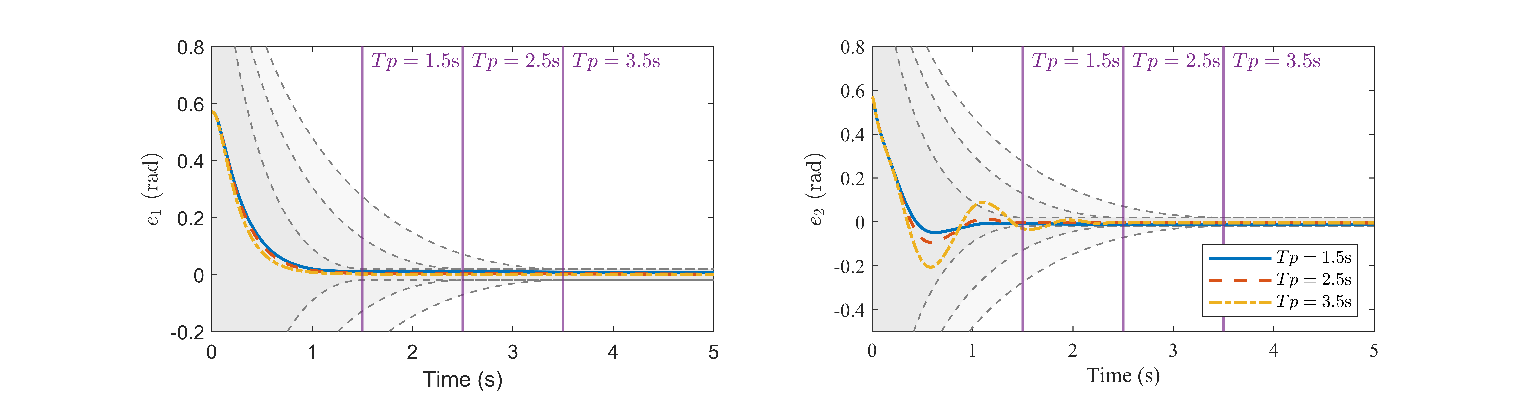
\includegraphics[width=0.9\linewidth]{fig3.eps}
% 	\caption{Position tracking errors under different predefined times \(T_p\).}
% 	\label{fig:3}
% \end{figure}

% \begin{figure}[H]
% 	\centering
% 	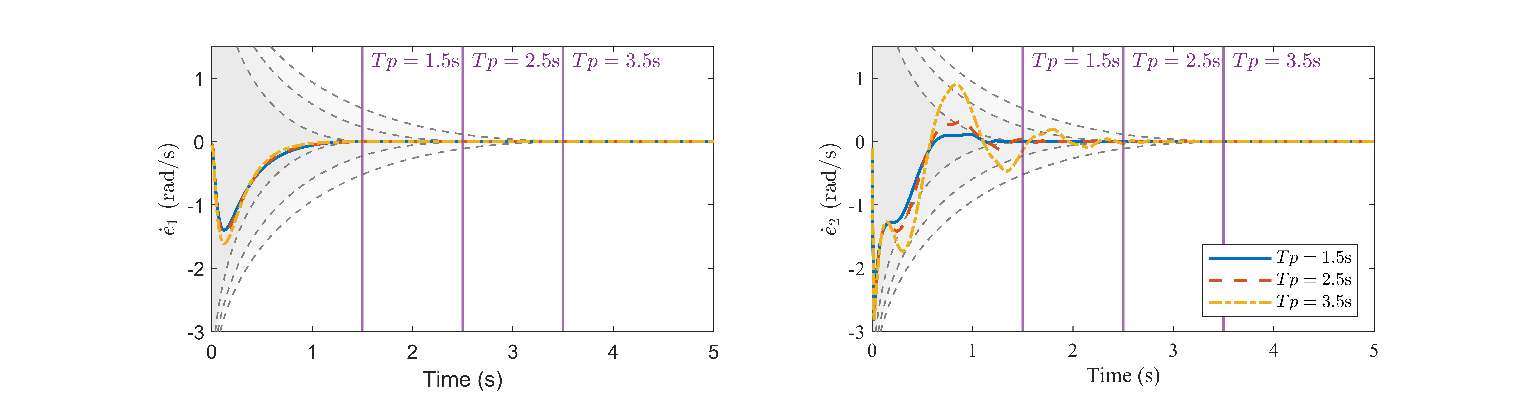
\includegraphics[width=0.9\linewidth]{fig4.eps}
% 	\caption{Velocity tracking errors under different predefined times \(T_p\).}
% 	\label{fig:4}
% \end{figure}

% % \begin{figure}[H]
% % 	\centering
% % 	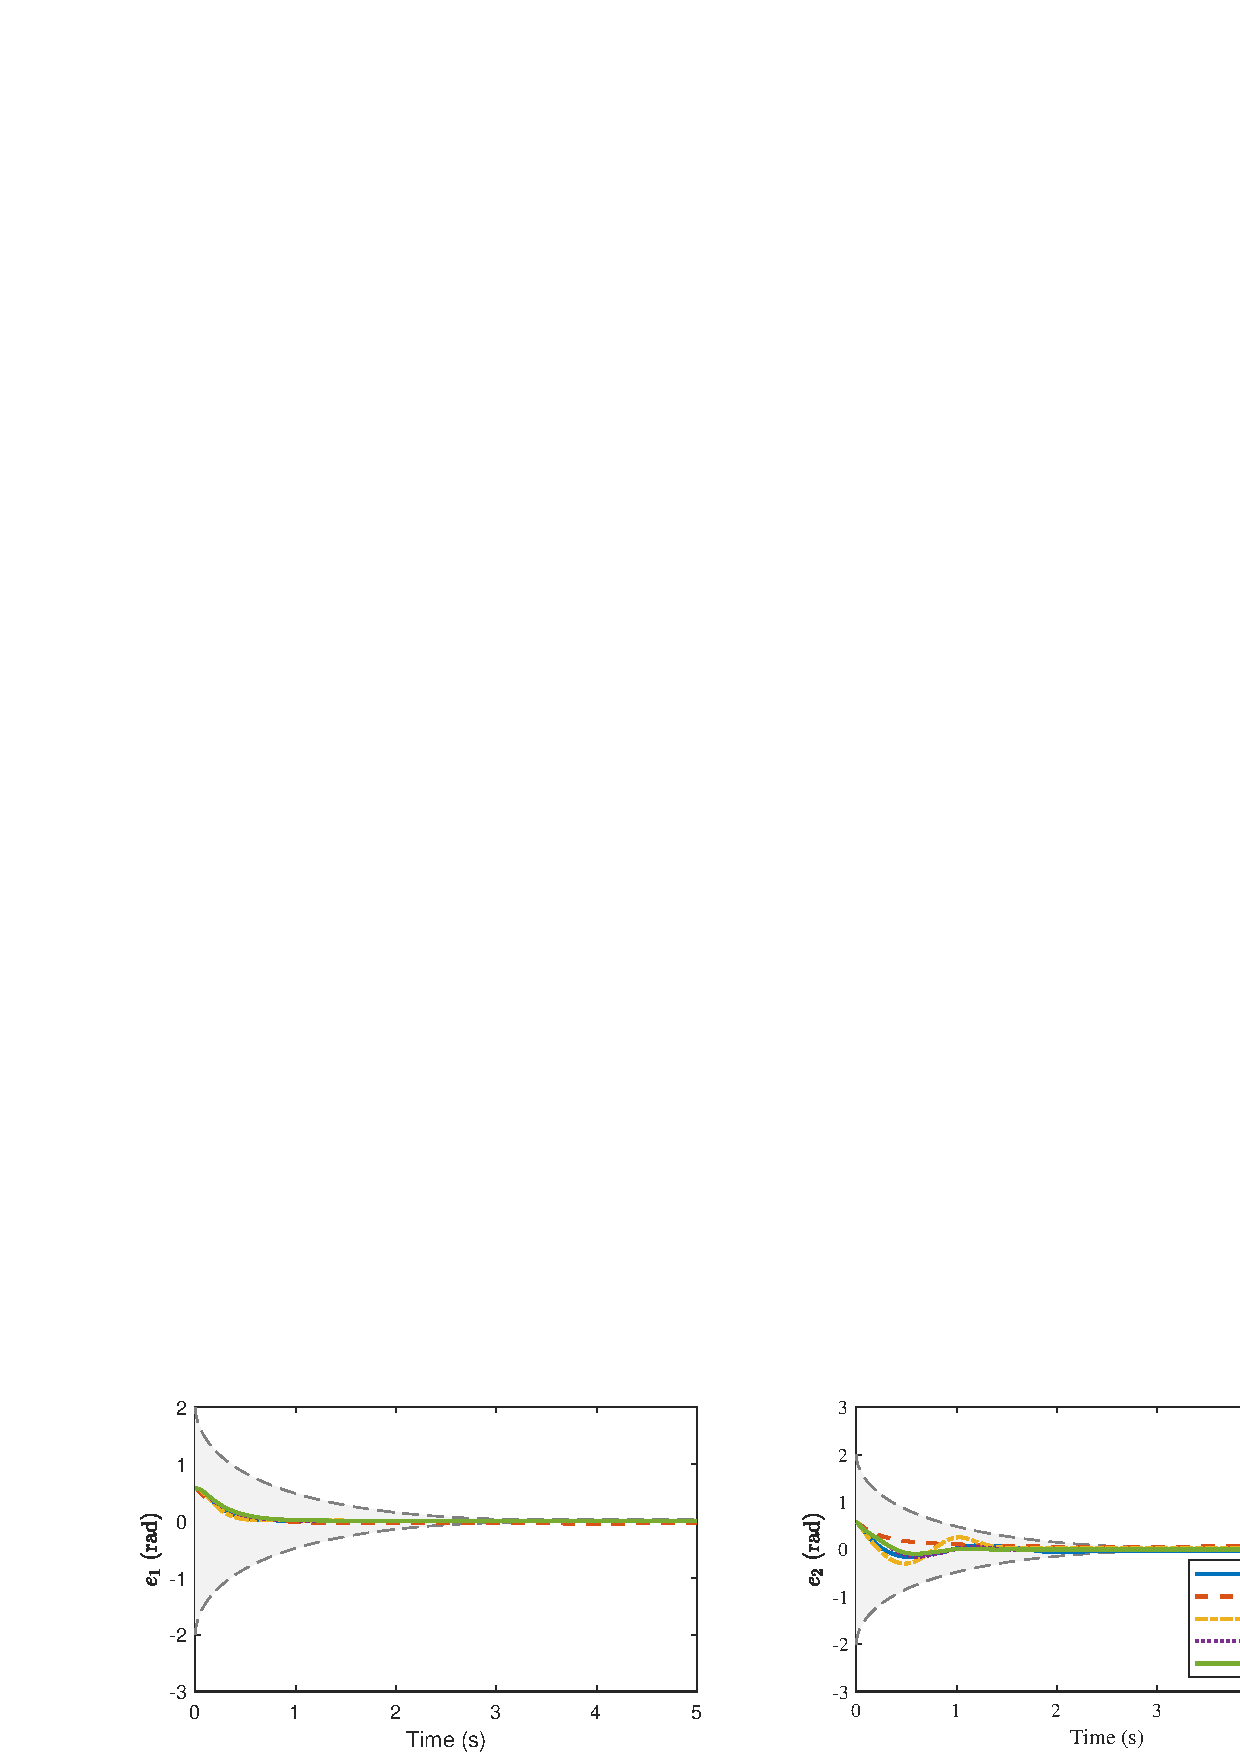
\includegraphics[width=0.9\linewidth]{fig9.jpg}
% % 	\caption{Velocity tracking errors under different predefined times of \(T_p\).}
% % 	\label{fig:9}
% % \end{figure}
% % \begin{figure}[H]
% % 	\centering
% % 	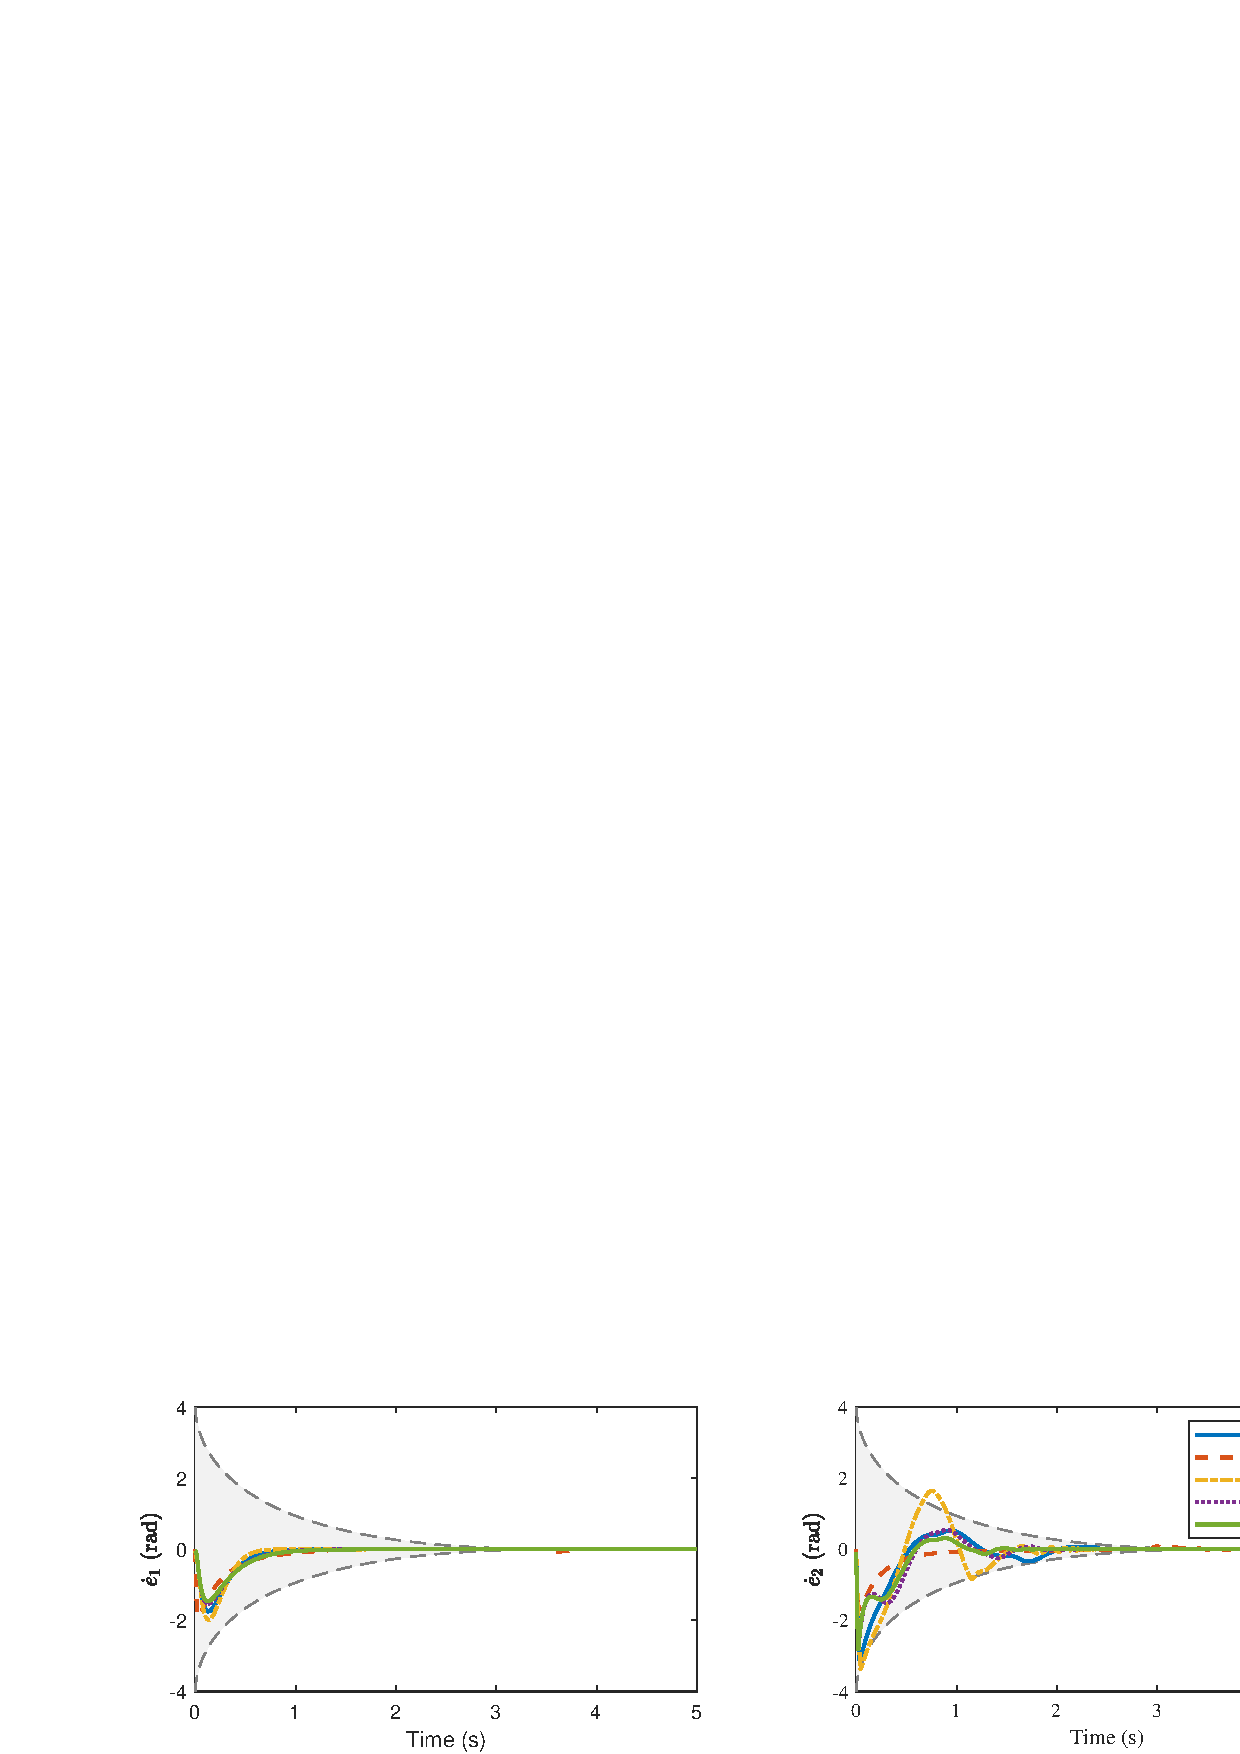
\includegraphics[width=0.9\linewidth]{fig10.jpg}
% % 	\caption{Velocity tracking performance under different predefined times of \(T_p\).}
% % 	\label{fig:10}
% % \end{figure}

% \begin{figure}[H]
% 	\centering
% 	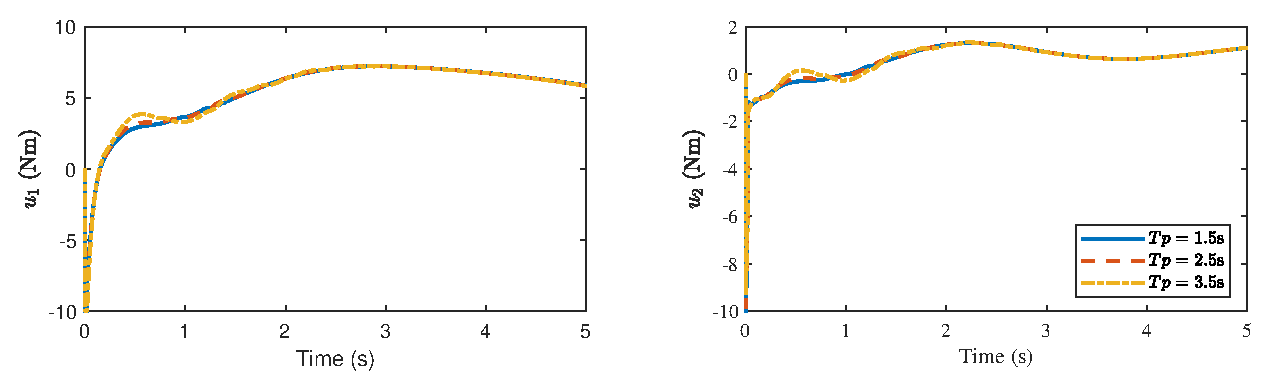
\includegraphics[width=0.9\linewidth]{fig5.eps}
% 	\caption{Control input torques under different predefined times \(T_p\).}
% 	\label{fig:5}
% \end{figure}


% \subsubsection*{Case 2: Different initial state conditions}

% % 在本实验中,我们分析了不同初始状态对控制性能的影响,尤其关注在考虑输入饱和与补偿机制下,预定义时间收敛性能是否仍然保持一致。仿真统一设置预定义时间为$T_p = 2.5\ \mathrm{s}$,初始状态分为两类:一类误差初始值在性能函数包络之内,$x_1(0) \in \left\{\left[{\pi}/{2}, {\pi}/{2}\right], \left[{\pi}/{4}, {\pi}/{4}\right], [0, \pi/2]\right\}$,另一类误差初始值超出性能函数上界,$x_1(0) \in \left\{ [\pi, \pi], \left[{-\pi}/{2}, {-\pi}/{2}\right],  \left[{-3 \pi}/{4}, {-3 \pi}/{4}\right]\right\}$。 

% % 从图 \cref{fig:6,fig:7} 可见,在初始误差处于性能包络内时,系统实现了快速且平稳的轨迹跟踪,误差曲线在 $T_p$ 之前光滑地收敛至零附近,速度响应亦无明显抖动,控制力矩幅度适中。这说明当误差初始值合理设置时,系统状态能在无需额外激励的情况下自然衰减,表现出理想的瞬态与稳态特性。当初始状态明显越界甚至远离目标轨迹时,误差轨迹在前 $0.5–1.5 \mathrm{s}$ 内迅速穿入性能包络区间,并且依然能够在 $T_p = 2.5\ \mathrm{s}$ 内完成系统收敛过程。控制力矩曲线如图 \cref{fig:8} 所示,在早期存在较大幅度的输入,但随后迅速下降,说明控制器在面对较大误差初值时快速生成足够强的初始驱动力,从而将误差推入约束区间,并维持稳定性。该实验结果充分验证,无论系统初始状态误差是否位于性能包络之内,所提出的控制器均能确保在预定义时间 $T_p$ 内实现误差的合法化与全局收敛。这表明系统具备与初始条件无关的时间收敛特性。

% To assess how initial states affect control performance under input saturation and its compensation, we fix the predefined-time at $T_p=2.5\,\mathrm{s}$ and test two classes of initial conditions: in-envelope $x_1(0)\in\{[\pi/2,\pi/2]^{\!\top},[\pi/4,\pi/4]^{\!\top},[0,\pi/2]^{\!\top}\}$ and out-of-envelope $x_1(0)\in\{[\pi,\pi]^{\!\top},[-\pi/2,-\pi/2]^{\!\top},[-3\pi/4,-3\pi/4]^{\!\top}\}$. The results in \cref{fig:6,fig:7,fig:8} show that, for in-envelope cases, the system achieves fast and smooth tracking: errors decay to near zero before $T_p$, velocity responses exhibit no noticeable ripple, and torque magnitudes remain moderate. For out-of-envelope cases, errors enter the prescribed envelope within $0.5\!-\!1.5\,\mathrm{s}$ and still converge by $T_p$; torques are larger early on but drop quickly, indicating strong initial drive followed by stabilization. These findings confirm that, with input saturation and anti-saturation compensation, the proposed controller ensures error “legalization” (entry into the envelope) and global convergence within $T_p$ regardless of the initial condition, i.e., the time of convergence is independent of the initial state.

% \begin{figure}[H]
% 	\centering
% 	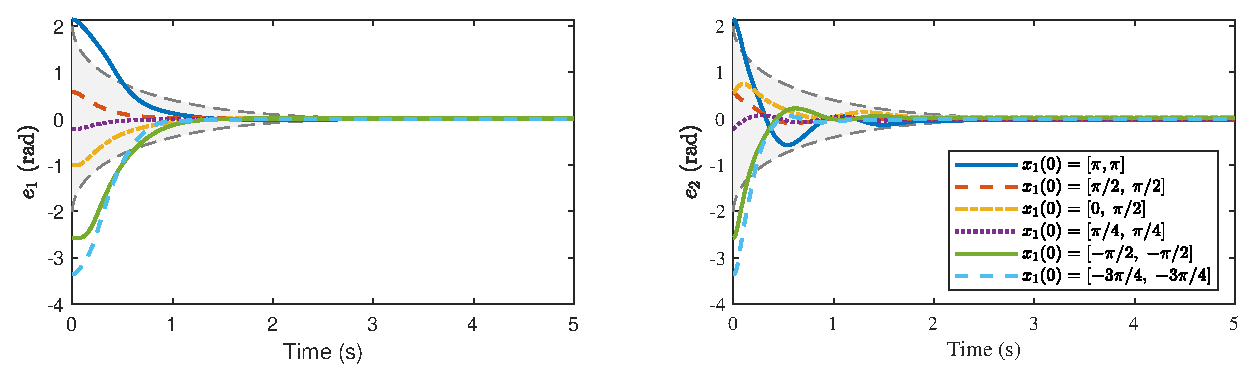
\includegraphics[width=0.9\linewidth]{fig6.eps}
% 	\caption{Position tracking errors under different initial values of \(x_1(0)\).}
% 	\label{fig:6}
% \end{figure}

% \begin{figure}[H]
% 	\centering
% 	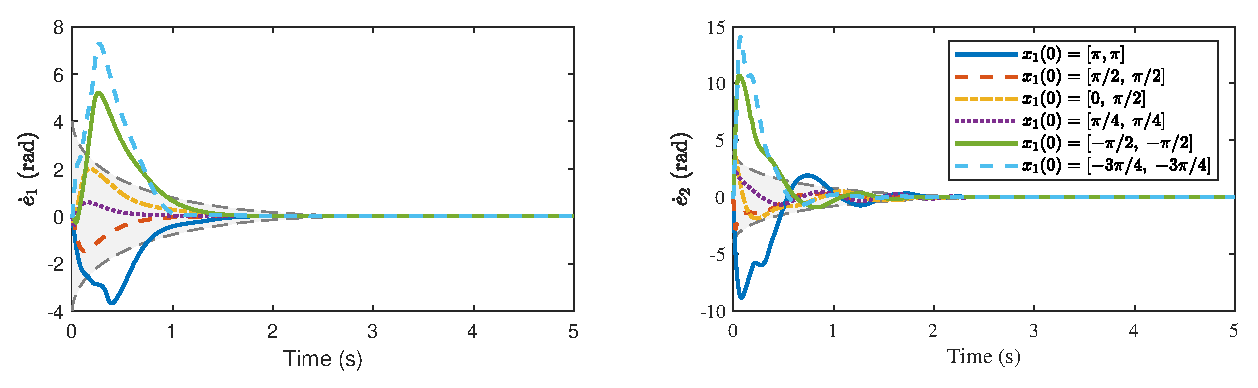
\includegraphics[width=0.9\linewidth]{fig7.eps}
% 	\caption{Velocity tracking errors under different initial values of \(x_1(0)\).}
% 	\label{fig:7}
% \end{figure}
% % \begin{figure}[H]
% % 	\centering
% % 	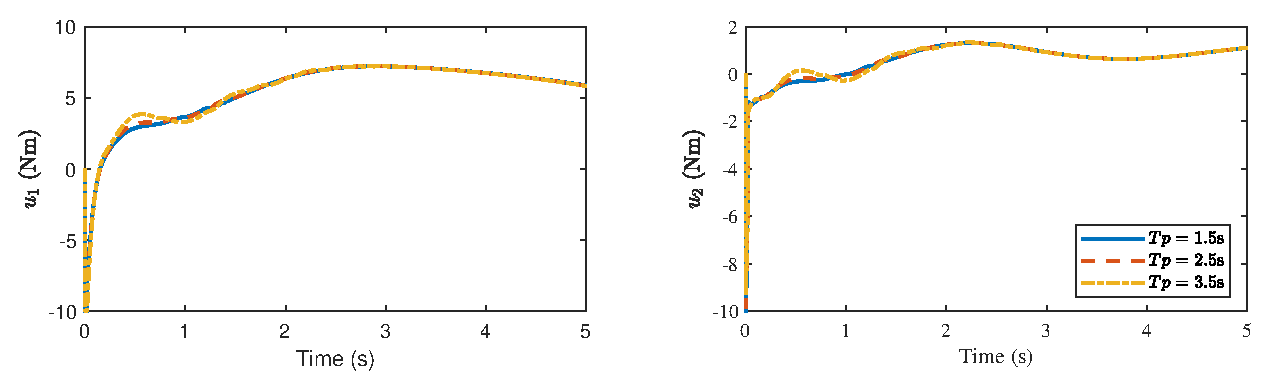
\includegraphics[width=0.9\linewidth]{fig5.eps}
% % 	\caption{Velocity tracking errors under different initial values of \(x_1(0)\).}
% % 	\label{fig:4}
% % \end{figure}

% % \begin{figure}[H]
% % 	\centering
% % 	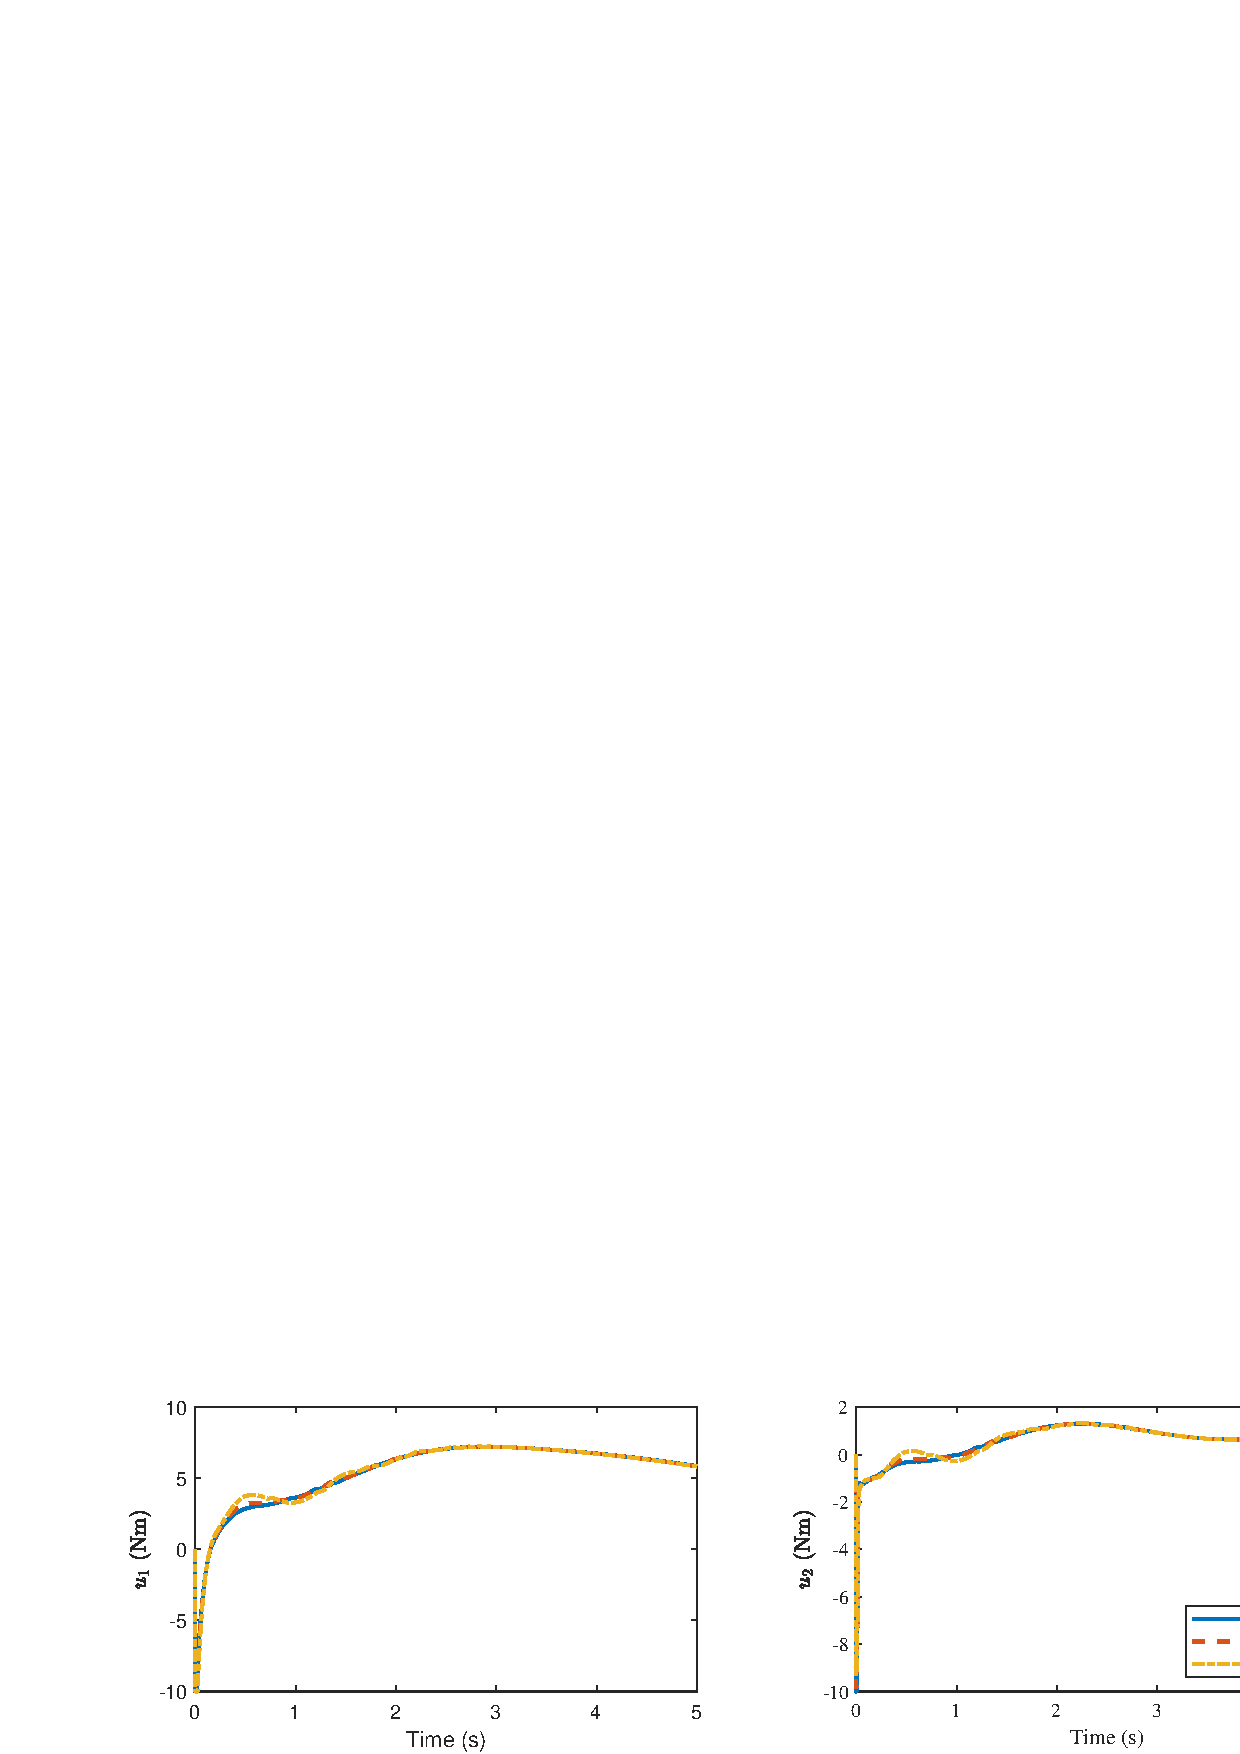
\includegraphics[width=0.9\linewidth]{fig5.jpg}
% % 	\caption{Velocity tracking performance under different initial values of \(x_1(0)\).}
% % 	\label{fig:5}
% % \end{figure}

% \begin{figure}[H]
% 	\centering
% 	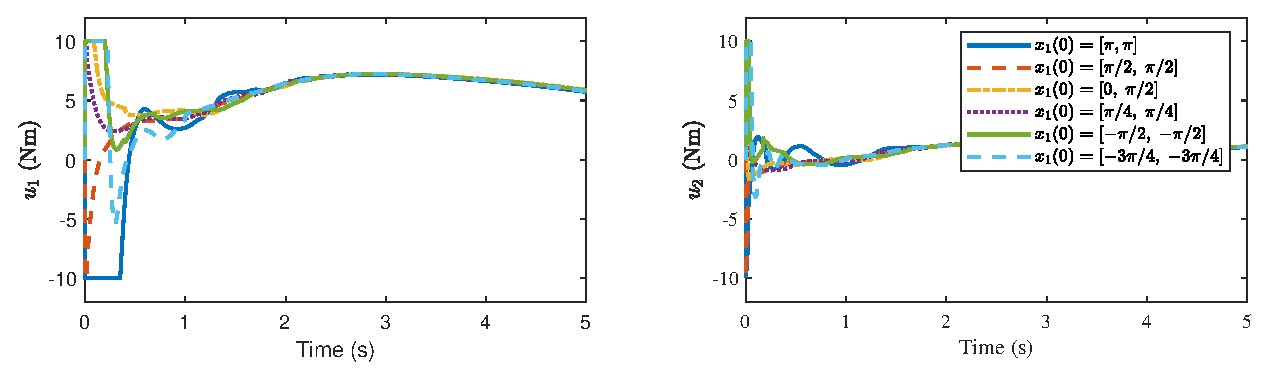
\includegraphics[width=0.9\linewidth]{fig8.eps}
% 	\caption{Control input torques under different initial value of \(x_1(0)\).}
% 	\label{fig:8}
% \end{figure}




% \subsubsection*{Case 3: Comparison of algorithms}

% % 为了验证所提出控制方法的综合性能优势,本文将其与三种控制策略进行了对比,包括无预设性能约束的预定义时间控制方法(PTC)、基于预设性能约束的渐近稳定控制方法(PPC)、参考文献\cite{CaoEtAl_2023_ReinforcementLearningBased} 中的固定时间收敛方法(FTC),预设性能约束的预定义时间控制方法(PTPPC)、以及本文所提出控制方法(Proposed)。其中 PTC和本文方法的预定义时间设为$T_p=2.5 \mathrm{s}$. 各方法在两组不同初始状态下进行仿真, $x_1(0) = [\pi/2, \pi/2]^{\top}$图 \cref{fig:9,fig:10,fig:11} , $x_1(0) = [-\pi/2, -\pi/2]^{\top}$(图 \cref{fig:9,fig:10,fig:11,fig:12,fig:13,fig:14} )。

% % 为全面评估所提出控制方法的综合性能优势,我们选取了四类具有代表性的控制策略作为对比对象:无性能约束的预定义时间控制(PTC)、基于预设性能的渐近稳定控制(PPC)、固定时间控制方法(FTC,参考文献 \cite{CaoEtAl_2023_ReinforcementLearningBased}),以及预设性能约束下的预定义时间控制方法(PTPPC)。本文所提方法(Proposed)则融合了基于位移函数的预设性能、预定义时间以及输入饱和补偿等关键特性。统一设置预定义时间 $T_p = 2.5\,\mathrm{s}$,并分别在两组初始状态下进行仿真测试:一组为 $x_1(0) = [\pi/2,\ \pi/2]^{\top}$(中等初始误差,\cref{fig:9,fig:10,fig:11} ),另一组为 $x_1(0) = [-\pi/2,\ -\pi/2]^{\top}$(偏离较大误差,图 \cref{fig:12,fig:13,fig:14})。

% % 从图 \cref{fig:9,fig:10,fig:11} 可见,PPC 方法在稳态控制上比较平滑,但收敛速度较慢;FTC 方法表现出较快收敛趋势,但存在不规则跳变和误差回弹,系统稳定性欠缺。PTC 方法虽然能在 $T_p$ 时间内实现收敛,但初始误差波动较大。相比之下,PTPPC 方法能够在 $T_p$ 时间内将误差压缩至规定范围内,控制输入较为平滑。本文所提方法进一步在此基础上引入了误差位移函数和饱和补偿,不仅确保了误差在整个过程中始终被性能包络约束,而且在收敛速度、控制平滑性和执行器能耗三方面表现最优,控制力矩无明显抖动或过冲。

% % 在初始状态为 $[-\pi/2,\ -\pi/2]^{\top}$ 的强越界情况下(图 \cref{fig:12,fig:13,fig:14}),各控制方法间性能差异更加显著。可以看出,PTC 和 FTC 方法在误差大幅偏离初始包络时出现了明显的震荡和短时发散现象,尤其是 FTC 方法控制力矩波动范围甚至长时间到达上限值,不利于实际执行器应用。PPC 和 PTPPC 方法由于缺乏对初始越界误差的快速调节能力,几乎无法实现有效跟踪,误差在整个过程中长期滞留在性能边界之外,控制力矩非常振荡但调节作用明显不足。相比之下,本文提出的方法在大初始误差和饱和约束并存的挑战下,仍能在预定义时间内实现误差合法化与稳定收敛,控制输入有界、平滑,展现出极强的鲁棒性与综合控制性能。


% To comprehensively evaluate the proposed method, we compare four representative controllers: predefined-time control without performance constraints (PTC), prescribed-performance asymptotic  stability control (PPC), fixed-time control (FTC, see \cite{CaoEtAl_2023_ReinforcementLearningBased}), and predefined-time control with prescribed-performance constraints (PTPPC). Our method (Proposed) combines a displacement-based performance shaping function, predefined-time regulation, and anti-saturation compensation. We fix $T_p=2.5\,\mathrm{s}$ and test two initial conditions: $x_1(0)=[\pi/2,\ \pi/2]^\top$ (in-envelope error, \cref{fig:9,fig:10,fig:11}) and $x_1(0)=[-\pi/2,\ -\pi/2]^\top$ (out-of-envelope error, \cref{fig:12,fig:13,fig:14}).

% For the in-envelope error case (\cref{fig:9,fig:10,fig:11}), PPC yields smooth steady-state behavior but slow convergence; FTC converges faster yet shows irregular jumps and rebounds; PTC meets the time target but exhibits large initial fluctuations. PTPPC compresses the error within the prescribed bounds by $T_p$ with relatively smooth inputs. Building on this, the Proposed controller—via the error-shift function and anti-saturation compensation—keeps the error within the envelope throughout, achieves faster convergence, smoother actuation, and lower actuator effort, with no noticeable torque overshoot or chattering.

% For the out-of-envelope error case (\cref{fig:12,fig:13,fig:14}), differences are amplified. PTC and FTC display pronounced oscillations and short-term divergence; FTC often drives torques to their limits for extended periods. PPC and PTPPC lack rapid correction for out-of-envelope initial errors, leaving the error outside the bounds and producing highly oscillatory inputs with limited regulation. In contrast, the Proposed method still legalizes the error and ensures stable convergence by $T_p$, with bounded and smooth inputs, demonstrating strong robustness and superior overall performance.


% \begin{figure}[H]
% 	\centering
% 	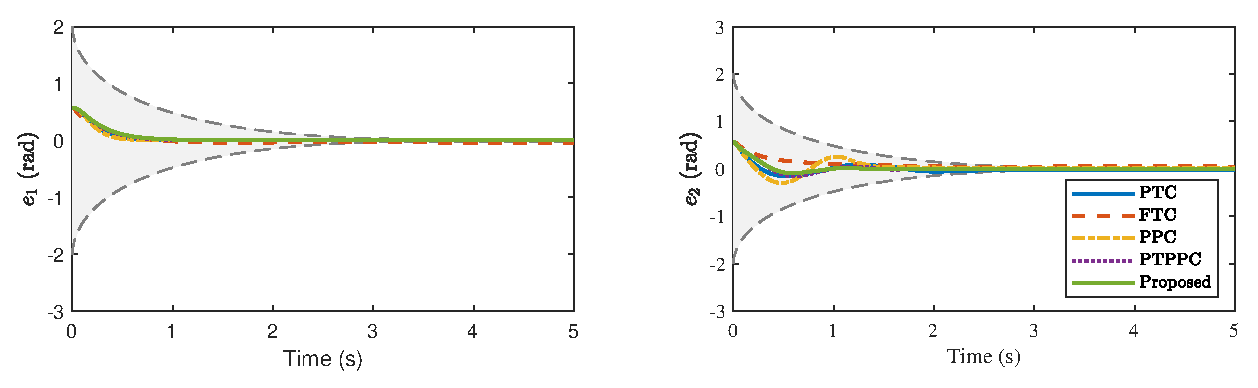
\includegraphics[width=0.9\linewidth]{fig9.eps}
% 	\caption{Comparison of position tracking errors under different methods with in-bound initial errors.}
% 	\label{fig:9}
% \end{figure}

% \begin{figure}[H]
% 	\centering
% 	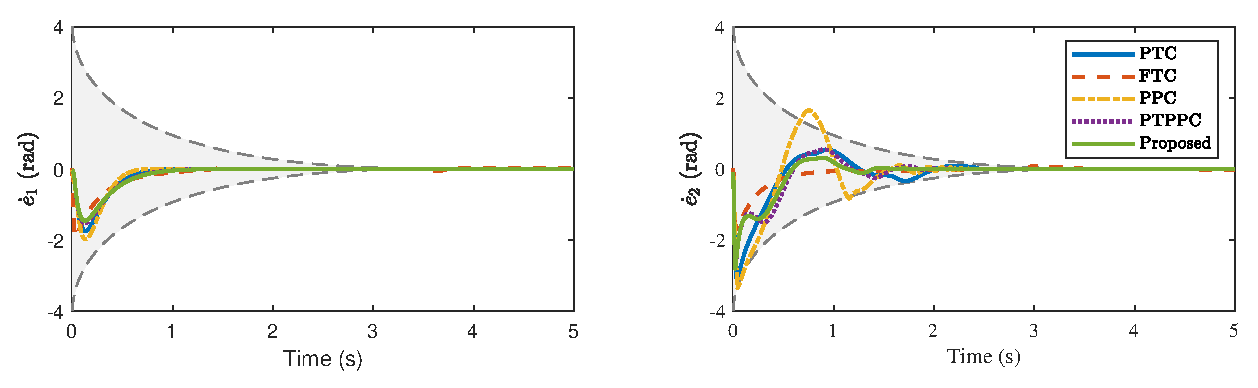
\includegraphics[width=0.9\linewidth]{fig10.eps}
% 	\caption{Comparison of velocity tracking errors under different methods with in-bound initial errors.}
% 	\label{fig:10}
% \end{figure}

% \begin{figure}[H]
% 	\centering
% 	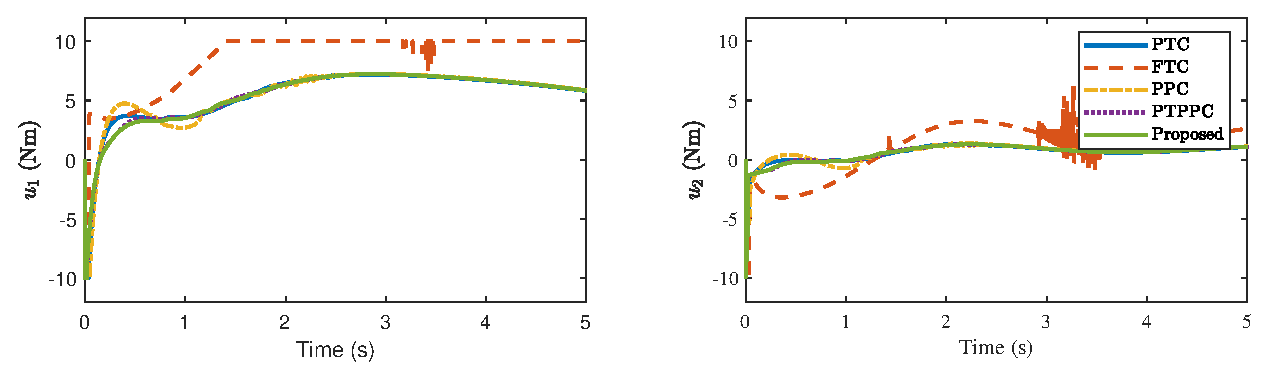
\includegraphics[width=0.9\linewidth]{fig11.eps}
% 	\caption{Comparison of control input torques under different Methods with in-bound initial errors.}
% 	\label{fig:11}
% \end{figure}

% \begin{figure}[H]
% 	\centering
% 	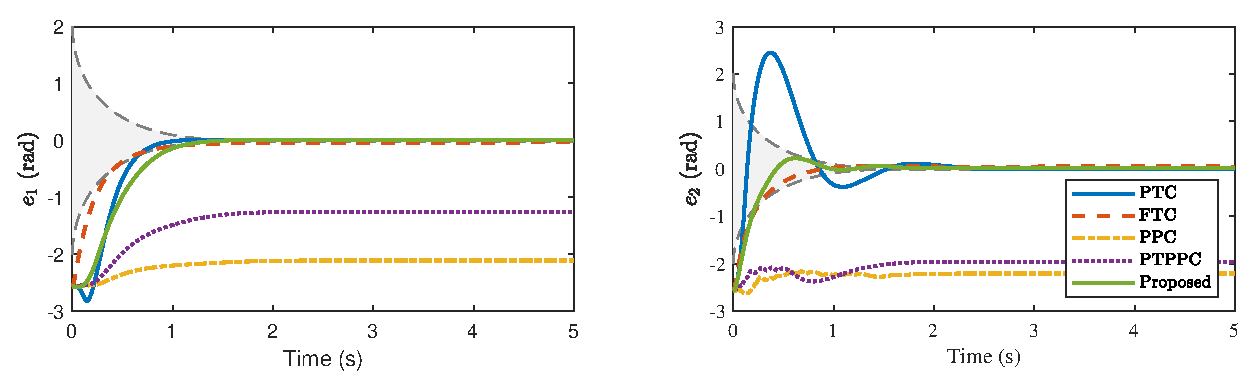
\includegraphics[width=0.9\linewidth]{fig12.eps}
% 	\caption{Comparison of position tracking errors under different methods with out-of-bound initial errors.}
% 	\label{fig:12}
% \end{figure}

% \begin{figure}[H]
% 	\centering
% 	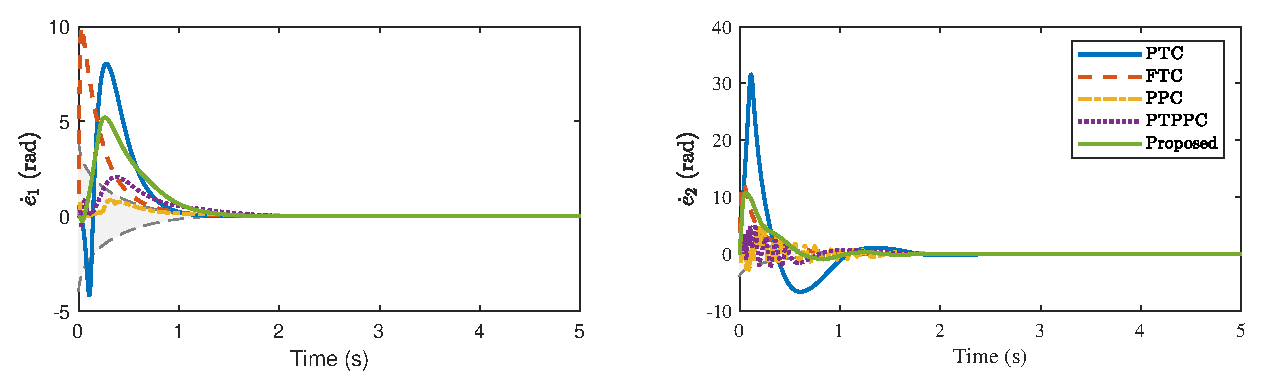
\includegraphics[width=0.9\linewidth]{fig13.eps}
% 	\caption{Comparison of velocity tracking errors under different methods with out-of-bound initial errors.}
% 	\label{fig:13}
% \end{figure}

% \begin{figure}[H]
% 	\centering
% 	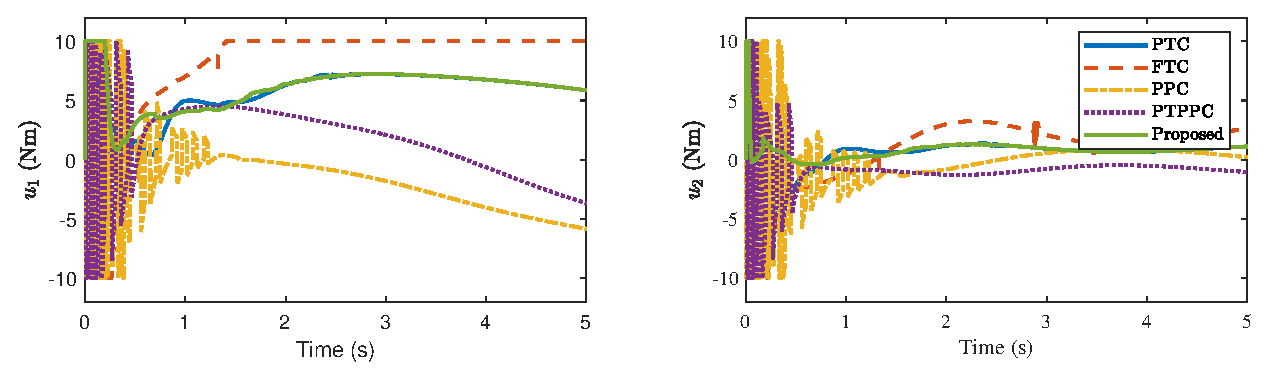
\includegraphics[width=0.9\linewidth]{fig14.eps}
% 	\caption{Comparison of control input torques under different Methods with out-of-bound initial errors.}
% 	\label{fig:14}
% \end{figure}



% \subsection{Experiment}

% % 为进一步验证本文提出控制方法在实际高自由度工业机器人系统中的有效性与通用性,本节选用 JAKA C7 型号的六自由度协作机械臂作为被控对象,开展六个关节的轨迹跟踪仿真实验。控制目标是使每个关节分别沿设定参考轨迹进行精确跟踪,同时保证所有跟踪误差在规定的预定义时间内收敛,并始终满足给定的性能边界约束。
% To further validate the effectiveness of the proposed method in real high DOF industrial robotic systems. A 6-DOF collaborative manipulator of JAKA C7 as shown in \cref{fig:15} is selected as the controlled object to carry out the trajectory tracking simulation experiments of six joints. The control objective is to enable each joint to track accurately along a set reference trajectory, while ensuring that all tracking errors converge within a specified predefined-time and always satisfy the given performance boundary constraints.

% The parameters of prescribed performance function are set as $p=0.6, \rho_1(0)=\pi/2, \rho_1(\infty )=0.02,\rho_2(0)=\pi, \rho_2(\infty )=0.02$. The predefined convergence time is set $T_p = 3\ \mathrm{s}$.
% The controller parameters are set as: $c=0.6$, $\gamma=0.4$, $\alpha_{\min}=-100, \alpha_{\max}=100$, $\lambda=2.5$, $\omega_{\min}=2, \omega_{\max}=6$, The control input is $u_{\min}=-u_{\max}, u_{\max}=[60; 60; 40; 30; 20; 15]$, $k_1=\mathrm{diag}( 30, 30, 30, 24, 24, 30) $, $k_2=\mathrm{diag}(12, 10, 12, 10, 8, 8)$. The remaining parameters are set consistent with those in the simulation subsection.
% The desired joint trajectories are constructed to cover a range of frequency components and are defined as follows
% $q_d(t)=[
% 			0.1\sin(0.5t) + \cos(0.5t),    
% 			0.1\sin(t) + \cos(t),          
% 			0.2\sin(1.5t) + 0.8\cos(t) ,   
% 			0.3\sin(2t) + 0.7\cos(0.5t),  
% 			0.1\sin(0.3t) + 0.9\cos(0.2t),
% 			0.4\sin(t) + 0.6\cos(2t)    
% 		]
% $.

% % 为了验证本文提出的控制方法的有效性,在典型的六自由度机械臂系统上,分别设计了四种控制器进行对比仿真:无性能约束的预定义时间控制(PTC)、基于预设性能的渐近稳定控制(PPC)、以及预设性能约束下的预定义时间控制方法(PTPPC);本文提出的方法(Proposed)。其中,Proposed 方法在 PTPPC 的基础上,进一步引入了位移函数调制机制与抗饱和补偿器。在实验过程中,以 $T_p = 3\,\mathrm{s}$ 作为预定义收敛时间,并设定性能包络 $\rho_i(t)$。The initial values of the robot manipulators are ${q_{d}}(0)=[{\pi}/{2}, -{\pi}/{2},{\pi}/{3}, -{\pi}/{3},{\pi}/{2},-{\pi}/{2}]$ rad, $\dot{q_{d}}(0)=\mathbf{0}$ rad/s. 需要强调的是关节 2、4、6 的初始误差明显大于各自的性能约束最大值,而关节 1、3、5 则位于性能约束以内。由此产生两类截然不同的动态:① 对于包络外的 2、4、6 轴,控制器首先必须快速把误差“拉回”边界;② 对于包络内的 1、3、5 轴,则直接按照性能函数约束衰减。\cref{Fig:16} 与 \cref{Fig:18} 显示,为不同算法的瞬态响应提供了直接对照。

% To validate the effectiveness of the proposed control method, we conduct comparative simulations on a representative 6-DOF manipulator model with four controllers: predefined-time control without performance constraints (PTC), prescribed-performance asymptotic stability control (PPC), predefined-time control with prescribed-performance constraints (PTPPC), and the proposed controller (Proposed). We fix the predefined-time at $T_p=3\,\mathrm{s}$ and specify jointwise performance envelopes $\rho_i(t)$. The initial values of the the manipulator are ${x}(0)=[{\pi}/{2}, -{\pi}/{2},{\pi}/{3}, -{\pi}/{3},{\pi}/{2},-{\pi}/{2}]$ rad, $\dot{x}(0)=\mathbf{0}$ rad/s. Importantly, the initial errors of joints 2, 4, and 6 exceed their respective bounds, whereas joints 1, 3, and 5 start within the envelopes, yielding two distinct dynamics: (i) for joints 2/4/6, the controller must first drive the errors back inside the bounds before tracking; (ii) for joints 1/3/5, the errors decay directly under the prescribed performance. The transient responses across algorithms are presented side by side in \cref{fig:16,fig:17,fig:18,fig:19,fig:20}.

% % \begin{equation}
% % 	\begin{aligned}
% % 		q_d(t) & =
% % 		\begin{bmatrix}
% % 			0.1\sin(0.5t) + \cos(0.5t),    \\  % 关节1:低频主导
% % 			0.1\sin(t) + \cos(t),          \\       % 关节2:中频
% % 			0.2\sin(1.5t) + 0.8\cos(t) ,   \\ % 关节3:混合频率
% % 			0.3\sin(2t) + 0.7\cos(0.5t),   \\% 关节4:高低频组合
% % 			0.1\sin(0.3t) + 0.9\cos(0.2t), \\% 关节5:超低频
% % 			0.4\sin(t) + 0.6\cos(2t)      % 关节6:交叉频率
% % 		\end{bmatrix},
% % 	\end{aligned}
% % \end{equation}

% \begin{figure}[H]
% 	\centering
% 	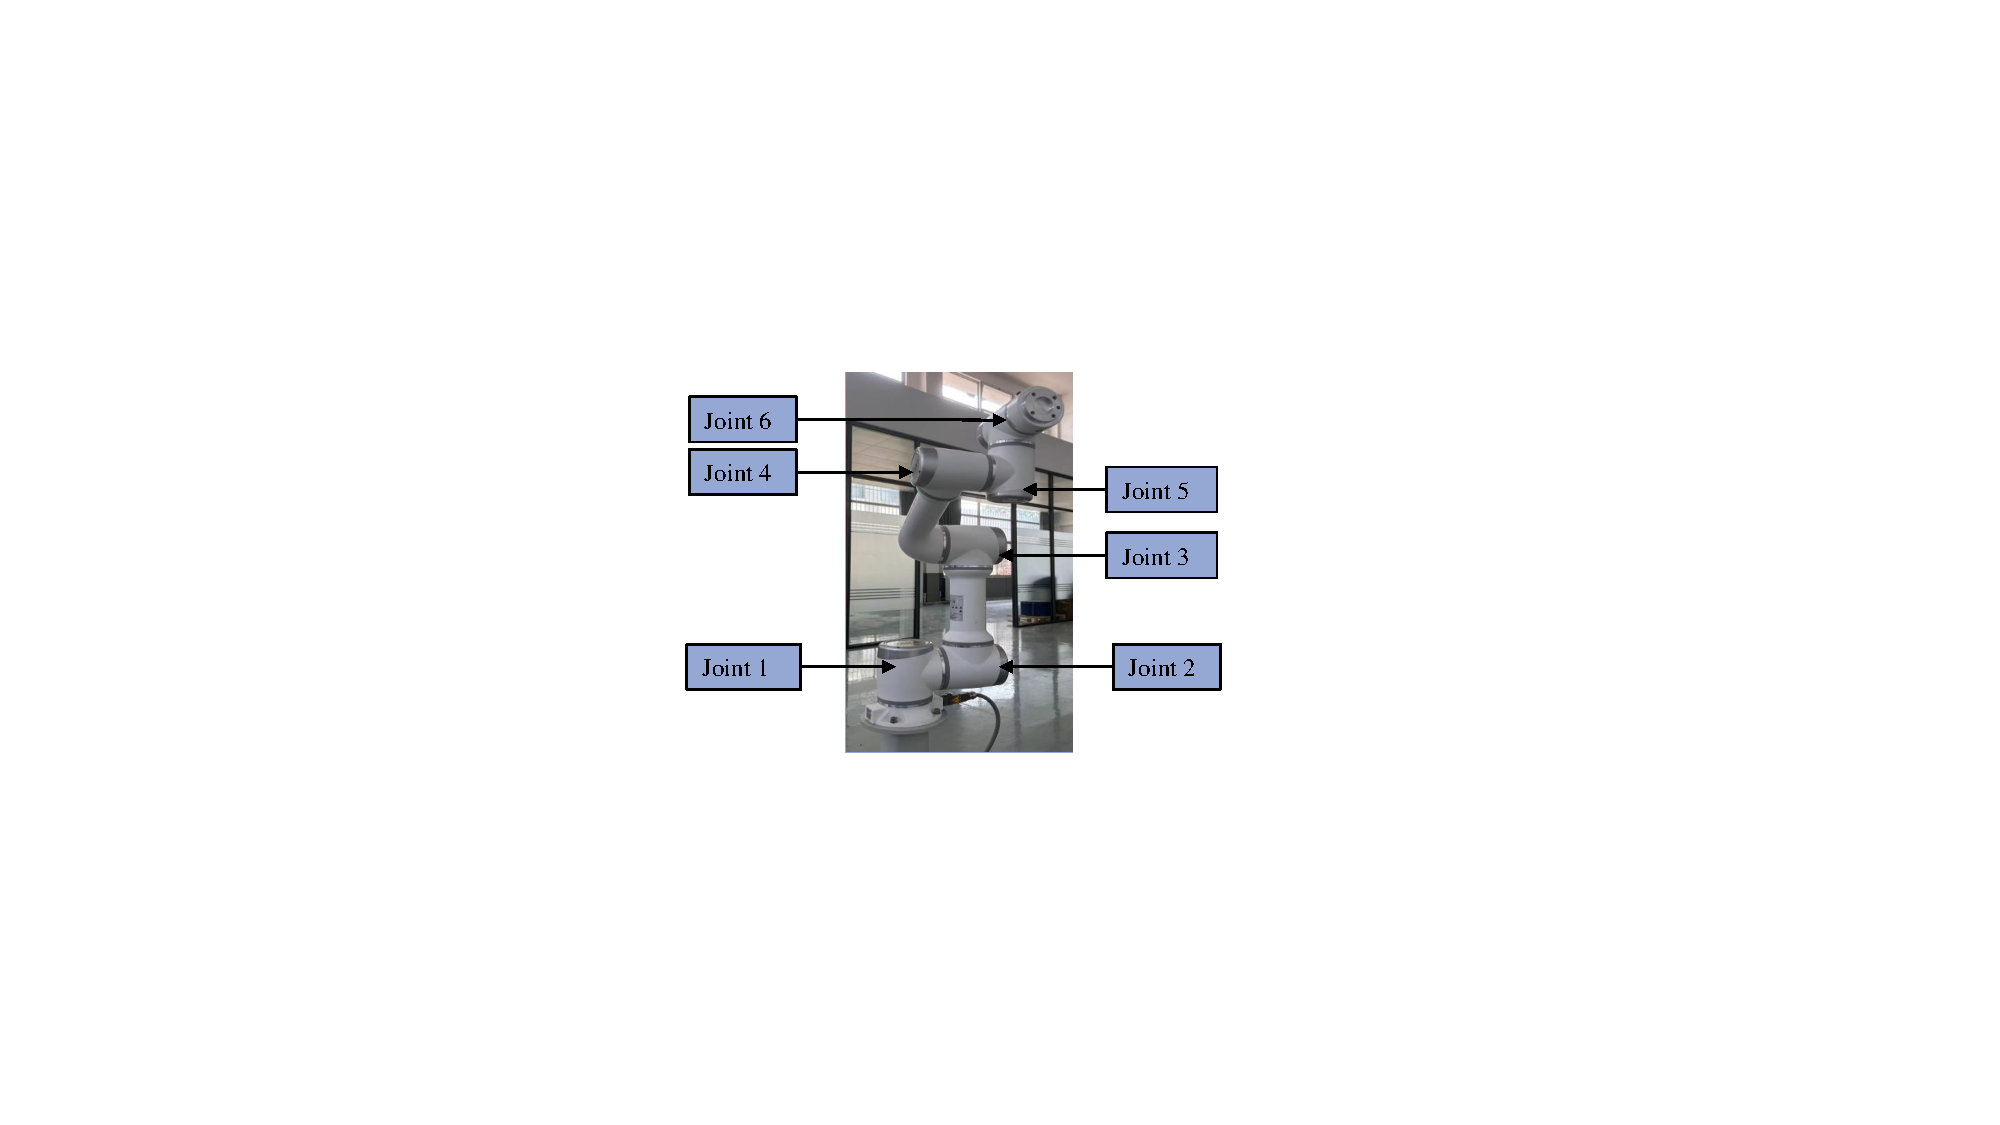
\includegraphics[width=0.4\linewidth]{fig15.pdf}
% 	\caption{The 6-DOF collaborative manipulator of JAKA C7.}
% 	\label{fig:15}
% \end{figure}

% % \begin{table}[h!]
% % 	\centering
% % 	\caption{Comparison for four control methods}
% % 	\label{tab:1}
% % 	\begin{tabular}{lcccc}
% % 	\hline
% % 	\textbf{控制器} & \textbf{最大位置误差 $|e_q|_{\max}$ (rad)} & \textbf{调节时间 (s)} & \textbf{峰值力矩/额定 (\%)} \\
% % 	\hline
% % 	PTC       & 2.8403 & 2.534 & 50.00 \\
% % 	PPC       & 2.8396 & 2.840 & 50.00 \\
% % 	PTPPC     & 2.8356 & 2.972 & 50.00 \\
% % 	Proposed  & 2.8094 & 3.861 & 50.00 \\
% % 	\hline
% % 	\end{tabular}
% % 	\end{table}


% \begin{figure}[H]
% 	\centering
% 	\includegraphics[width=0.9\linewidth]{fig16.eps}
% 	\caption{Comparison of position tracking errors under different methods of 6-DOF manipulator.}
% 	\label{fig:16}
% \end{figure}

% \begin{figure}[H]
% 	\centering
% 	\includegraphics[width=0.9\linewidth]{fig17.eps}
% 	\caption{Comparison of position tracking trajectories under different methods of 6-DOF manipulator.}
% 	\label{fig:17}
% \end{figure}

% \begin{figure}[H]
% 	\centering
% 	\includegraphics[width=0.9\linewidth]{fig18.eps}
% 	\caption{Comparison of velocity tracking errors under different methods of 6-DOF manipulator.}
% 	\label{fig:18}
% \end{figure}
% \begin{figure}[H]
% 	\centering
% 	\includegraphics[width=0.9\linewidth]{fig19.eps}
% 	\caption{Comparison of velocity tracking performance under different methods of 6-DOF manipulator.}
% 	\label{fig:19}
% \end{figure}

% \begin{figure}[H]
% 	\centering
% 	\includegraphics[width=0.9\linewidth]{fig20.eps}
% 	\caption{Comparison of Control input torques under different methods of 6-DOF manipulator.}
% 	\label{fig:20}
% \end{figure}


% % 在综合比较四种控制策略的试验结果后可以看出PTC 与 Proposed 均能在 $T_p = 3\,\mathrm{s}$ 内实现误差收敛,但 Proposed 由于额外引入位移函数调制与抗饱和补偿,其误差曲线几乎无超调、控制力矩更平滑,整体瞬态与稳态品质明显优于 PTC;PPC 虽满足预设性能框架,却因缺乏时间约束与饱和处理,位置与速度误差在 $0–2 \mathrm{s}$  内振荡幅度大、收敛速度最慢,且在 3 s后 时仍残留误差,无法满足时间指标;PTPPC 则对包络外的大初始误差响应不足,特别是关节 2、4、6 的误差始终滞留在性能函数之外,无法完成合法化过程。综合来看,Proposed 在收敛速度、稳态精度、抖振抑制与执行器负荷四个维度均显著优于 PTC、PPC 与 PTPPC。该协同设计不仅保证了时间-性能双重约束,还通过饱和补偿降低了能耗与热负荷,对大初始偏差及输入限幅并存的高自由度机械臂具有工程适用性。
% As shown in \cref{fig:16,fig:17,fig:18,fig:19,fig:20}, after a comprehensive comparison of the four controllers, both PTC and the Proposed method achieve convergence within $T_p=3\,\mathrm{s}$. However, thanks to the added displacement-function modulation and anti-saturation compensation, the Proposed method shows virtually no overshoot and much smoother torques, yielding clearly superior transient and steady-state quality to PTC. PPC complies with the prescribed-performance framework but, lacking explicit time enforcement and saturation handling, exhibits large oscillations in position/velocity errors during $0\text{–}2\,\mathrm{s}$, converges the slowest, and still leaves residual error after $3\,\mathrm{s}$, thus failing the time requirement. PTPPC responds poorly to large out-of-envelope initial errors; in particular, the errors of joints 2, 4, and 6 remain outside the bounds and the legalization step is not completed. Overall, the Proposed controller surpasses PTC, PPC, and PTPPC in convergence speed, steady-state accuracy, chattering suppression, and actuator load. The coordinated design enforces the time–performance dual constraints and, via saturation compensation, reduces energy consumption and thermal load, making it suitable for high-DOF manipulators with large initial deviations under input limits.

	

% \section{Conclusion}

% % 本文提出了一种融合预定义时间收敛理论与全局性能约束的自适应反步控制方法,用于解决具有未知动力学、有界扰动和输入饱和条件下的机器人机械臂轨迹跟踪问题。
% % 该方法提出了一种针对每个通道独立设计预定义时间误差变换结构,系统性地解决了传统预设性能控制方法中存在的初值奇异性和误差变换非光滑问题,确保系统在未知初始状态下满足误差的严格、平滑且全局的预定义时间约束。
% % 设计了一种统一的辅助补偿器信号,快速消除虚拟与实际输入间的饱和残差并抑制计算复杂性。
% % 引入了一阶滑模扰动观测器与基于RBFNN的未建模动态辨识与补偿机制,应对有界扰动和未建模动态的不利影响。
% % 理论分析证明了闭环系统在预定义时间内的稳定性和误差收敛性。
% % 仿真与实验结果表明,本文方法在初始误差快速处理、预定义时间内动态性能约束的实现、执行器转矩需求的降低等性能提升等方面均明显优于现有方法。
% % 未来将面向真实机器人平台与更复杂工况,包括参数不确定、通信与计算延迟、突发外扰与任务切换等开展验证,并探索与学习型策略的安全融合与可证收敛,以进一步提升在高自由度与多任务协作系统中的应用能力。


% This work proposes an adaptive backstepping controller that combines predefined-time convergence and global prescribed-performance constraints. The goal is trajectory tracking for manipulators with unknown dynamics, bounded disturbances, and input saturation. We design a channel-wise predefined-time error transformation. It removes initial-condition singularities and nonsmooth mappings in conventional PPC. It enforces strict, smooth, global bounds regardless of the initial state. We also add a unified auxiliary compensator. It quickly cancels saturation residuals between virtual and actual inputs and curbs computational growth. A first-order sliding-mode observer and an RBFNN estimator handle disturbances and unmodeled dynamics. Lyapunov analysis proves predefined-time stability and error convergence. Simulations and hardware experiments show clear gains over baselines. The method legalizes large initial errors fast, meets performance within the prescribed time, and reduces actuator torque. Future work will test on real robots under tougher conditions such as parameter drift, delays, abrupt disturbances, and task switching. We will also explore safe integration with learning-based methods with provable convergence for high-DOF, multi-task systems.





% \bibliographystyle{sn-mathphys-num}
\bibliography{sn-bibliography}

% \input{sn-article.bbl}
\section*{Statements and Declarations}
\subsection*{Funding}

This work is supported by the National Key Research and Development Program of China (2023YFC3008802), the National Natural Science Foundation of China (52075465), and the Key Products of Hunan Province's Manufacturing Industry "Unveiled and Leading" Project (2023GXGG018), the Project of Scientific Research Fund of the Hunan Provincial Science and Technology Department (2023JJ50021, 2023GK2029, No.2024JC1003, No.2024JJ1008, 2024JJ2051, 2023GK2026), "Algorithmic Research on Mathematical Common Fundamentals" Program for Science and Technology Innovative Research Team in Higher Educational Institutions of Hunan Province of China, the Hunan Provincial Department of Education Excellent Youth Program (23B0162).

\subsection*{Conflicts of Interest}
The authors declare no conflict of interest.

\subsection*{Author contribution}
Shuli Liu: Writing-Original Draft, Methodology, Software, Visualization, Data curation. Yi Liu:Resources, Investigation, Formal analysis, Conceptualization, Writing-Review \& Editing. 
Jingang Liu: Project administration, Validation, Funding acquisition, Writing-Review \& Editing. 
Yin Yang: Supervision, Funding acquisition, Writing-Review \& Editing. 
All authors have reviewed and approved the final version of the manuscript.
\subsection*{Data Availability}
The data that support the findings of this study are available from the corresponding author upon reasonable request.

\end{document}


